\documentclass[5p,twocolumn,10pt,times]{elsarticle}
\usepackage{amsmath}
\usepackage{lineno, hyperref}
\modulolinenumbers[1]
%\linenumbers
%\addtolength{\textheight}{8mm}
%\addtolength{\textwidth}{4mm}
%\addtolength{\voffset}{-10mm}
%\addtolength{\hoffset}{-3mm}

\bibliographystyle{elsarticle-num-names}


% ACM template
%
%\documentclass[acmtog,anonymous,timestamp,review]{acmart}
%
%\usepackage{booktabs} % For formal tables
%


% !TeX spellcheck = en_GB 


% My TK added packages and commands

	\newif\ifcolorrevise
	
	\colorrevisetrue

	% for for using hyperref and elsarticle-num-names together in order to get \citeauthor to work
	\makeatletter
	\providecommand{\doi}[1]{%
	  \begingroup
	    \let\bibinfo\@secondoftwo
	    \urlstyle{rm}%
	    \href{http://dx.doi.org/#1}{%
	      doi:\discretionary{}{}{}%
	      \nolinkurl{#1}%
	    }%
	  \endgroup
	}
	\makeatother

	% have multiline subfigure captions be centered
	\usepackage[labelformat=parens]{subcaption} % subfigures
	\captionsetup[subfigure]{justification=centering}
	\captionsetup{subrefformat=parens} % pure refernce subfigure with parentheses: fig.10a and (b)
	%\renewcommand\thesubfigure{(\alph{subfigure})} % refernce subfigure always with parentheses: fig.10(a) and (b)

	\captionsetup[figure]{labelfont={bf},name={Fig.},labelsep=period} % use `Fig.' for figure subscript instead of `Figure'
	
	\usepackage[export]{adjustbox} % [right] alignment for includegraphics
	
	\usepackage{rotating} % turn env for rotating text in figures

	\usepackage{wrapfig} % inline figures

	% tables
	\usepackage{multirow} % multicolumn, multirow
	\usepackage{colortbl} % \cellcolor{<color>}
	\newcolumntype{C}[1]{>{\centering\arraybackslash}m{#1}}   %% centered
	\newcolumntype{R}[1]{>{\raggedleft\arraybackslash}m{#1}}  %% right aligned

	\usepackage[capitalise]{cleveref} % automatically add `Fig.'  etc before a reference.

        \usepackage{ amssymb } % \therefore
	
	\newcommand{\degree}{^\circ}
	
	\usepackage[binary-units]{siunitx} % mm and stuff
	\sisetup{per-mode = symbol}
	\DeclareSIUnit\pixel{px}

	\usepackage{units} % \nicefrac{3}{8}
	
	\usepackage{ stmaryrd } % mathmode \lightning
	
	\DeclareMathOperator*{\argmax}{arg\,max}
	\DeclareMathOperator*{\argmin}{arg\,min}
	
	\DeclareMathOperator{\abs}{abs} % absolute function

	\usepackage{amsthm} % \begin{proof}
	\newtheorem{lemma}{Lemma}[section]
	\theoremstyle{definition}
	\newtheorem{definition}{Definition}[section]

	\usepackage[inline]{enumitem} % inline enumerate*

	\usepackage[toc,page]{appendix} % appendicces
	
	\usepackage{pgfplots}
	\usepackage{pgfplotstable} % tikzpicture table plots
	\pgfplotsset{compat=1.15}
	\usetikzlibrary{backgrounds}

	\usepackage[noend]{algpseudocode} % algorithmic
	\usepackage{algorithm} % wrapper for pseudocode to give a caption and label

	\newcommand{\pluseq}{\mathrel{+}=} %pluseq symbol
	\usepackage{upgreek} % \uplambda

	\usepackage{listings} % for listing C++ code instead of pseudocode
	\lstset{ 
      breaklines=true,                 % sets automatic line breaking
      basicstyle=\ttfamily,
      mathescape
    }




    % \usepackage[disable]{todonotes} % notes not showed  
    % \usepackage[draft]{todonotes}   % notes showed
    \usepackage{color,soul} % caps, highlight (\hl)

	\newcommand{\comment}[1]{}
	
    \newcommand{\todo}[1]{\hl{#1}}
    
	\newcommand{\temp}[1]{\textcolor[rgb]{0, 0, 0.2}{#1}}
	\newcommand{\tim}[1]{\temp{\todo{[Tim: #1]}}}
	\newcommand{\jun}[1]{\temp{\todo{[Jun: #1]}}}
	
	\newcommand{\old}[1]{\textcolor{gray}{#1}}
	\usepackage[normalem]{ulem}
	\newcommand{\stkout}[1]{\ifmmode\text{\sout{\ensuremath{#1}}}\else\sout{#1}\fi}
	
	% Revise macro (usage: \revise{old}{new})
	\newcommand{\revise}[2]{#2}
	% Version a) First arg red and striked out, second argument green
	%\newcommand{\revise}[2]{\textcolor{red}{\stkout{#1}}\textcolor{blue}{#2}}
	%\newcommand{\revise}[2]{{\color{red}{#1}\color{blue}{#2}}}
	% Version b) First arg ignored, second argument green
	\ifcolorrevise
	\renewcommand{\revise}[2]{{\color{blue}{#2}}}
	\fi
	% Version c) First arg ignored, second argument unchanged (for final draft)
	%\newcommand{\revise}[2]{#2}
	%\newcommand{\revise}[2]{#1}

	\newcommand{\outdated}[1]{{\color{red}{#1}}}

	\setulcolor{red}

	\usepackage[normalem]{ulem} % squigly underline

	\renewcommand\floatpagefraction{.8}


	\newlength{\figwidth}
	\newlength{\figwidthTwo}
	\newlength{\figwidthTree}
	\newlength{\figheight}
	\newlength{\figheightTwo}
	\newlength{\tempheight}
	\newlength{\tempheightTwo}

	% deal with missing images which are not directly included in the repo
	\iftrue
	\newcommand{\noimage}[1]{%
	  \setlength{\fboxsep}{-\fboxrule}%
	  \fbox{\phantom{\rule{10pt}{10pt}} Missing file: \path{#1} \phantom{\rule{10pt}{10pt}}}% Framed box
	}
	\let\includegraphicsoriginal\includegraphics
	\renewcommand{\includegraphics}[2][width=\textwidth]{\IfFileExists{#2}{\includegraphicsoriginal[#1]{#2}}{\noimage{#2}}}

	\fi
% ENd of TK's added packages and commands



\begin{document}
\baselineskip11pt 

\begin{frontmatter} 

\title{ITIM: Interlaced Topologically Interlocking Microstructure for continuous dual-material extrusion}

%\author{Paper ID: xxx}

\author[um,tud]{Tim Kuipers}
\author[man]{Renbo Su}
\author[tud]{Jun Wu\corref{cor1}}
\ead{j.wu-1@tudelft.nl}
\cortext[cor1]{Corresponding author}
\author[man]{Charlie C. L. Wang}
% \ead{cwang@mae.cuhk.edu.hk}
\address[um]{Ultimaker, Utrecht, The Netherlands}
\address[tud]{Department of Sustainable Design Engineering, Delft University of Technology, The Netherlands}
\address[man]{Department of Mechanical, Aerospace \& Civil Engineering, The University of Manchester, United Kingdom}


\begin{abstract}
Fused deposition modelling (FDM) 3D printing has developed over the recent years from a tool used for prototyping to a tool for manufacturing end-use products.
Being able to print with multiple materials unlocks applications where different parts have different requirements.
However, when chemically incompatible materials are used the adhesion between two materials can be negligible.
In order to affix two bodies of incompatible materials a common strategy is to design mechanically interlocking structures at the interface between the two.

Existing literature considers only 2D interlocking dovetail structures for FDM 3D printing.
3D interlocking with high genus topology locks all 3 dimensions by linking closed loops of both materials together comparable to a chain mail.
The interlock is therefore less affected by the material's tendency to deform under stress.
Requiring a high genus topology to satisfy extrusion continuity constraints appears challenging.

We propose a simple and effective interlocking microstructure consisting of interlaced beams in two directions which constitute a high genus topology: the interlaced topologically interlocking microstructure (ITIM).
We develop general analytical models for optimizing the ultimate tensile strength of the ITIM lattice in two different orientations w.r.t. the interface.
The general analytical models are applied to polypropylene (PP) and polylactic acid (PLA) and verified by FEM simulations and physical tensile experiments.
In the diagonal orientation ITIM can obtain 82\% of the theoretical upper bound of \SI{8.6}{\mega\pascal}, which is 67\% of the ultimate tensile strength of the PP and slightly higher than the strength obtained using dovetail designs.
If the length of the transition region is limited to less than \SI{2.4}{\milli\meter} the straight orientation is expected to outperform the diagonal orientation of the ITIM lattice.

%Expanding this research to interlocking structures optimized for non-vertical interfaces and non-horizontal forces is an interesting direction for future research.

\end{abstract}

%
% The code below should be generated by the tool at
% http://dl.acm.org/ccs.cfm
% Please copy and paste the code instead of the example below.
%
%\begin{CCSXML}
%\end{CCSXML}

%\ccsdesc[500]{Computer systems organization~Embedded systems}
%\ccsdesc[300]{Computer systems organization~Redundancy}
%\ccsdesc{Computer systems organization~Robotics}
%\ccsdesc[100]{Networks~Network reliability}

\begin{keyword} 
keywords
\end{keyword}

\end{frontmatter}




\newcommand{\hc}{h_\text{c}}
\newcommand{\hf}{h_\text{f}}
\newcommand{\w}[1]{w_{#1}}
\newcommand{\wa}{w_{a}}
\newcommand{\wb}{w_{b}}
\newcommand{\wm}{w_{m}}
\newcommand{\va}{v_{a}}
\newcommand{\vb}{v_{b}}
\newcommand{\vm}{v_{m}}
\newcommand{\hmin}{h_\text{min}}
\newcommand{\wmin}[1]{w_{\text{min}, #1}}
\newcommand{\lmax}{L_\text{max}}
\newcommand{\mt}[1]{M_{\text{T}}^#1}
\newcommand{\myz}[1]{M_{\text{XX}}^#1}
\newcommand{\mxz}[1]{M_{\text{XZ}}^#1}
\newcommand{\mxy}[1]{M_{\text{XY}}^#1}

\newcommand{\stresstensile}[1]{\sigma_{\text{XX}, #1}}
\newcommand{\stresszshear}[1]{\tau_{\text{XY}, #1}}
\newcommand{\stresscrossshear}[1]{\tau_{\text{XZ}, #1}}
\newcommand{\sigmafail}[1]{\sigma_{\text{y}, #1}}
\newcommand{\sigmafailz}[1]{\sigma_{\text{yZ}, #1}}
\newcommand{\taufail}[1]{\tau_{\text{y}, #1}}
\newcommand{\tauz}[1]{\tau_{\text{yZ}, #1}}



\newcommand{\gwa}{g_\text{wa}}
\newcommand{\gwb}{g_\text{wb}}
\newcommand{\gva}{g_\text{va}}
\newcommand{\gvb}{g_\text{vb}}
\newcommand{\ghf}{g_\text{hf}}
\newcommand{\gd}{g_\text{d}}
\newcommand{\gta}{g_\text{ta}}
\newcommand{\gtb}{g_\text{tb}}
\newcommand{\gtm}{g_\text{tm}}
\newcommand{\gca}{g_\text{ca}}
\newcommand{\gcb}{g_\text{cb}}
\newcommand{\gza}{g_\text{za}}
\newcommand{\gzb}{g_\text{zb}}
\newcommand{\gzm}{g_\text{zm}}
\newcommand{\gtabroken}{g_{\text{ta}\lightning}}
\newcommand{\gtbbroken}{g_{\text{tb}\lightning}}
\newcommand{\gcbbroken}{g_{\text{cb}\lightning}}
\newcommand{\gzabroken}{g_{\text{zb}\lightning}}


%  \temp{%Table of contents just for reviewing purposes
% \tableofcontents
%  }

\section{Introduction}

Intuitively it seems impossible to generate high genus interlocking geometry while enforcing continuous extrusion for both materials;
if the one material leaves a hole in a layer then filling that hole with the other material will cause it to be disconnected from the other regions of the second material.



Our contributions are as follows:
\begin{itemize}
	\item A high genus interlocking structure for continuous extrusion
	\item A similar structure optimized for bending
	\item A similar structure optimized for tensile pulling
\end{itemize}


% !TeX spellcheck = en_GB 
\section{Related Work}


\subsection{Microstructures}
% multi-material microstructures
Microstructures such as beam lattices, triply periodic surfaces and ordered dithering have widely been studied for their mechanical properties\cite{Cadman2013,Zhang2018a,tamburrino2018}.
Single material microstructures can constitute auxetic materials, or light weight structures with tailored material properties, through fine adjustments of the microstructure geometry.
Such microstructures are often manufactured using stereolithography and polyjetting, because of these processes have very few manufacturing constraints.
Microstructures are inherently high genus, which makes them good candidates for interlocking\cite{freund2019determination}.
However, optimizing microstructures for adhesions between incompatible materials while adhering to FDM manufacturing constraints has been studied scarcely.



\subsection{Adhesion}

Important factors for adhesion between polymers are entanglement and dissipation\cite{abbott2015adhesion}.
The adhesion by which two bodies of different FDM printed material stick together can be influences by a wide spectrum of pre-treatment methods, process parameters and material properties\cite{freund2019determination}.
Increasing surface roughness might improve the adhesion between materials\cite{huttenbach1991interface,gent1990model}, but this supposed benefit is contested\cite{abbott2015adhesion}.
For FDM one could try mixing the materials by overlapping their toolpaths to increase adhesion or create simple straight protrusions in order to increase the friction between the two materials\cite{tamburrino19}.
However, if such protrusions bulge outward the adhesions doesn't merely increase through friction, but also because it would constitute a dovetail type of interlocking structure.

% Cura 4.8 allows for generating sandwich structures where the layers are alternated between the two materials.


\subsection{Interlocking in FDM}

%\subsubsection{Dovetail interlocking}
Literature on interlocking patterns for adhesion between incompatible materials in FDM 3D printing has focussed on extruded 2D interlocking dovetail type of designs,
such as jigsaw shapes ($\Omega$)\cite{malik2017}, trapezoidal sutures ($\sqcap$)\cite{Li2013}, T-shapes\cite{Ribeiro2019}, star shapes ($\bigstar$)\cite{Wang2021} in the horizontal direction
as well as in the vertical direction across several layers\cite{debora2020}.
Topology optimization can generate complex 2D dovetail interlocking shapes, which fit to the specifics of the design locally\cite{aharoni2021}.
Such interlocking designs are extrusions of 2D shapes and therefore they allow for translation along the extrusion axis, so these type of interlocking designs don't lock all axes.

The jigsaw idea can be expanded into a 3D interlocking structure by protruding not only sideways, but also vertically, resulting in a shape which looks like a tree ($\clubsuit$)\cite{gouker2006manufacturing}.
Similarly the T-shaped interlocking design can be expanded with beams in the vertical directions as well as the horizontal bars of the T.
However, such designs violate the semi-continuous extrusion requirement because the layers above and below the base of the T contain separated islands of one material, 
which are difficult to print when the two materials don't adhere to each other.

%\subsubsection{Genus interlocking}
These issues can be addressed by generating a repeating microstructure where the interlocks are connected together to form a high genus topology which locks all degrees of freedom.
Simple straight I shaped extrusions can be linked together by cross beams in order to form a genus interlocking structure\cite{Rossing2020}.
In their application where the second material is overmolded silicone the manufacturing constraints don't hold,
but in cases where the second material is also 3D printed, the space enclosed by the cross beams and extruded walls forms an island and thereby violates the extrusion continuity constraint.
A different microstructure is required if the extrusion continuity constraint is to be met for both materials.

%%  Single material adhesion structures
%The mechanical properties of single material 3D prints can also be improved by techniques similar to interlocking.
%By injecting material which span several layers the inter-layer bonding can be improved\cite{Duty2019,Kazmer2020}.
%Weaving extruded strands together across several layers is another technique to improve layer adhesion\cite{yao20213d}.




% !TeX spellcheck = en_US 
\section{Method}\label{interlocking:sec:method}
This paper considers topologically interlocking structures satisfying extrusion continuity constraints,
which will be optimized for tensile strength;
the geometry of the designs are optimized to yield or break at the highest horizontally applied tensile stress.
The highest administrable force applied to a unit cell of any interlocking structure will be carried by both materials $a$ and $b$.
In the plane where tensile failure of material $a$ occurs the total force $F$ will be distributed over the cross-sectional area $A_a$;
likewise for material $b$.
The theoretically optimal interlocking \revise{microstructure}{lattice} would be such that the force $F$ will be homogeneously distributed over $A_a$ and $A_b$
in such manner that both materials will fail at the same ultimate force: $F = \sigmafail{a} A_a = \sigmafail{b} A_b$.
\revise{The structure will break where the force is distributed of the smallest area $A_a$ or $A_b$, so increasing their overall size would improve on the \revise{microstructure}{lattice},
but}{The ultimate force before material $a$ breaks can be improved by increasing the area $A_a$, but this is at the cost of material $b$ (and vice versa), since} their combined area is limited to the total cross sectional area $A_\text{total}$ of the \revise{microstructure}{lattice}.
The ultimate strength of any multi-material \revise{microstructure}{lattice} is therefore limited to:

\begin{align}
	\sigma^* &= \frac{F}{A_\text{total}} 
	= \frac{F}{A_a + A_b}  \nonumber
	= \frac{\sigmafail{a} A_a}{A_a + A_b} \nonumber \\
	% = \frac{\sigmafail{b} A_b}{A_a + A_b} \nonumber \\
	%
	%\sigmafail{a} A_a &= \sigmafail{b} A_b \nonumber \\
	A_a &=  A_b \nicefrac{\sigmafail{b}}{\sigmafail{a} } \nonumber \\
\label{interlocking:eq:general_uper_bound}
	\sigma^*
	&= \frac{\sigmafail{a} A_b \nicefrac{\sigmafail{b}}{\sigmafail{a} } }{A_b \nicefrac{\sigmafail{b}}{\sigmafail{a} }  + A_b}
	%= \sigmafail{a} \frac{ \nicefrac{\sigmafail{b}}{\sigmafail{a} } }{ \nicefrac{\sigmafail{b}}{\sigmafail{a} }  + 1} \\
	%&= \frac{ \sigmafail{b} }{ \nicefrac{\sigmafail{b}}{\sigmafail{a} }  + 1} \\
	= \frac{ 1 }{ \nicefrac{1}{\sigmafail{a}} + \nicefrac{1}{\sigmafail{b}} } 
	%\approx \SI{8.6}{\mega\pascal} \text{ for PLA and PP}
\end{align}


This formula for the ultimate tensile strength of interlocking \revise{microstructure}{lattice}s is a theoretical upper bound.
In practice the worst cross-sectional area $A_a$ is in a different plane than the worst cross-sectional area $A_b$, so they do not add up to $A_\text{total}$.
For example, in the dovetail geometry (\cref{interlocking:fig:basic_2d_interlock}) the highest stress of a dovetail of material $a$ is at its base, while the highest stress in $b$ will be at the end of the dovetail of material $a$.
The geometry by which the interlock is secured reduces the strength compared to the theoretical upper bound of the ultimate tensile strength.
The upper bound can therefore never be reached.
% Moreover, the stress distribution will be heterogeneous when subjecting a complex geometry to tension.







\begin{figure*}
	\centering
	\begin{subfigure}[B]{.32\textwidth}
		\centering
		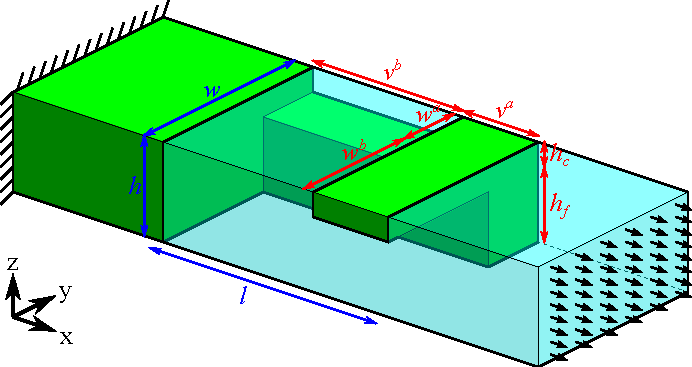
\includegraphics{sources-method-straight_model_v5_no_failures.pdf}
		\caption{Design variables (in red)}
		\label{interlocking:fig:straight_model}
	\end{subfigure}
	\begin{subfigure}[B]{.32\textwidth}
		\centering
		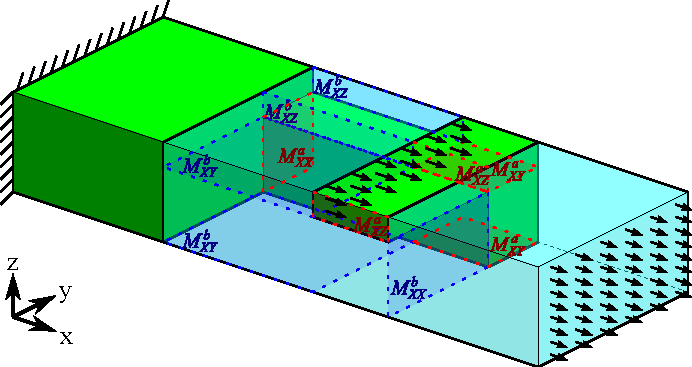
\includegraphics{sources-method-straight_model_v5_failures.pdf}
		\caption{Failures modes for material $a$ (in red) and for $b$ (in blue)}
		\label{interlocking:fig:straight_model_failure_modes}
	\end{subfigure}
	\begin{subfigure}[B]{.32\textwidth}
		\centering
		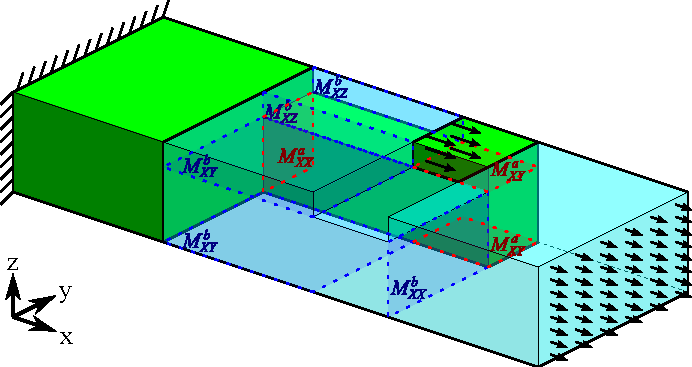
\includegraphics{sources-method-straight_model_v5_broken.pdf}
		\caption{Partly broken, partly interlocking cell}
		\label{interlocking:fig:straight_model_broken}
	\end{subfigure}
	\caption{Unit cell of the straight ITI\revise{M}{L} variant. Force is transferred from material $a$ (green) to material $b$ (transparent cyan) through the contact area on the cross beams. In the partly broken situation there is still interlocking, but the total force is transferred through a narrower area.}
\end{figure*}

\begin{figure*}
	\centering
	\begin{subfigure}[B]{.25\textwidth}
		\centering
		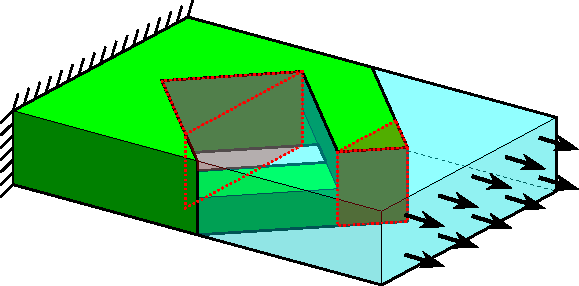
\includegraphics{sources-method-diagonal_model_simple_v5.pdf}
		\caption{Simple cell}
		\label{interlocking:fig:diagonal_model_simple}
	\end{subfigure}
	\begin{subfigure}[B]{.33\textwidth}
		\centering
		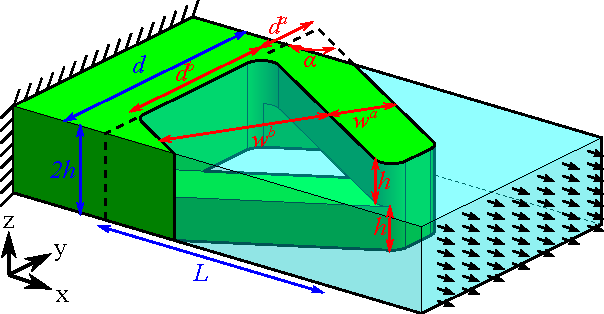
\includegraphics{sources-method-diagonal_model_v5_no_failures.pdf}
		\caption{Rounded and aligned design}
		\label{interlocking:fig:diagonal_model}
	\end{subfigure}
	\begin{subfigure}[B]{.33\textwidth}
		\centering
		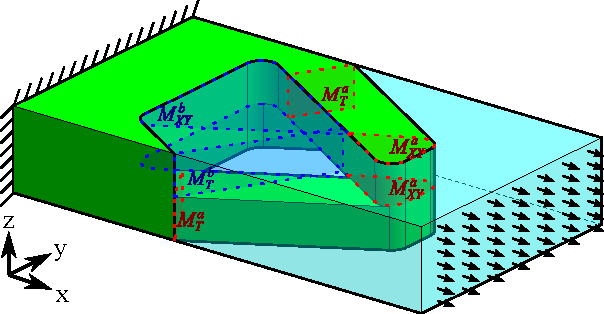
\includegraphics{sources-method-diagonal_model_v5_failures.pdf}
		\caption{Failure modes}
		\label{interlocking:fig:diagonal_model_failures}
	\end{subfigure}
	\caption{Unit cell of the diagonal ITI\revise{M}{L} variant. The $\mt{m}$ failure modes are orthogonal to the beams and influenced by both tensile and shear components of the total force.}
\end{figure*}




\subsection{Interlaced Topologically Interlocking \revise{Microstructure}{Lattice}}\label{interlocking:sec:itim}
The topologically interlocking structure we propose consists of horizontal beams alternating in material.
On top of that we print another set of beams rotated about Z and on top beams of the first rotation again, etc.
Long horizontal beams assure continuous extrusion, while the alternating direction of the beams assures the interlock.
See \cref{interlocking:fig:basic_structure_single_mat}.


When joining bodies of different materials, some region around the interface between the two bodies should be replaced by a number of unit cells from such a lattice structure.
The length of the transition region $L$ is limited by the design of the product within which the lattice is to be employed.
We consider a design constraint of $\lmax = 12 \wmin{m} = \SI{3.6}{\milli\meter}$;
this is enough to have some design freedom for the \revise{microstructure}{lattice}, while limiting the impact on the rest of the product.

With a relatively small length $\lmax$ it stands to reason to fill that space using a single unit cell in the length direction only.
If the same region were to be filled with 2 versions of the same cell but scaled to half lengthwise, then the total area of shear remains the same,
but the shear areas of the two cells would not bear the same load, so the stresses in one of the cells would only increase by using two cells instead of one.
One might consider using a different geometry for the two cells to counteract that fact,
but we do not expect such a multi-layered interlocking design to outperform a single layered interlocking lattice when $\lmax$ is relatively low. 

\revise{Given that we will fill the space around the interface with a single layer of cells, the orientation of those cells w.r.t. the interface is relevant.}{According to the reasoning above we should fill the interface with a single layer of cells, but how should those cells be oriented w.r.t. the interface?}
While rotating the lattice about X or Y is impossible due to the continuous extrusion constraint, we are free to rotate about Z.
However, given that the tensile stress is applied in a single direction it only makes sense to consider two orientations: straight and diagonal.


For the materials chosen by this study, Ultimaker Tough \revise{PLA}{Polylactic Acid} (\revise{T}{}PLA) and Ultimaker PolyPropylene (PP), the theoretical upper bound comes out to be \SI{8.6}{\mega\pascal}.
The structure may not only be subject to tensile failure, but also to shear failure modes.
Because of the layer-wise build-up employed by \revise{FDM}{MEX}, the tensile properties in the Z direction are different from those in the horizontal plane.
See \cref{interlocking:tab:mat_props_manufacturing_constraints}.
The structure is furthermore subject to manufacturing constraints determined by the nozzle sizes and the layer thickness.
The standard layer thickness $\hmin$ is \SI{0.1}{\milli\meter} and the minimal line width $\wmin{}$ for a \SI{0.4}{\milli\meter} nozzle is \SI{0.3}{\milli\meter}.


\begin{table}
	\caption{Yield properties of single material \revise{FDM}{MEX} printed samples.}
	\label{interlocking:tab:mat_props_manufacturing_constraints}
	\centering
	\begin{tabular}{l|rrrrrr}
		material & $\sigmafail{}$ & $\sigmafailz{}$ & $\epsilon_\text{y}$ & $\epsilon_\text{yZ}$ \\
		\hline
		\revise{T}{}PLA & \SI{47}{\mega\pascal} & \SI{33}{\mega\pascal} & \SI{3.5}{\percent} & \SI{2.6}{\percent}\\
		PP & \SI{10.5}{\mega\pascal} & \SI{10.6}{\mega\pascal} & \SI{29}{\percent} & \SI{22}{\percent}
	\end{tabular}
\end{table}


If all dimensions of the beams are set to minimal and the angle between the beams is set to \SI{90}{\degree},
%tensile tests show that the straight ITI\revise{M}{L} variant reaches \SI{3.3}{\mega\pascal} and the diagonal variant reaches \SI{4.9}{\mega\pascal}.
the finger of the straight ITI\revise{M}{L} variant takes up a quarter of the area at the base of the cell, so we can expect the strength to be close to $\nicefrac14 \sigmafail{b} \approx \SI{2.6}{\mega\pascal}$.
For the diagonal ITI\revise{M}{L} variant the beams take up half of the area at the base of the cell, which would be close to $\nicefrac12 \sigmafail{b} \approx \SI{5.3}{\mega\pascal}$.
However, these ultimate strengths can be improved upon considerably by optimizing the geometry.
This section considers these two ITI\revise{M}{L} variants and analytical models to optimize them.




\subsection{Straight ITI\revise{M}{L} variant}
A unit cell of the straight ITI\revise{M}{L} variant is visualized in \cref{interlocking:fig:straight_model}.
A cell consists of a single \emph{finger} of height $\hf$ protruding from the body of material $a$ outward and part of a \emph{cross beam} of height $\hc$ angled at \SI{90}{\degree}.
In order to print the relatively short fingers using continuous extrusion, we employ the constraints that $\wm \ge 2\wmin{m}$ (where $m$ is either material $a$ or $b$),
so that the toolpaths for the outline of each layer can go back and forth along the finger without interruption.
The cross beams are long and continuous enough, so they could be printed using a single extrusion path: $\vm \ge \wmin{m}$.
We set the minimum height of the beams to twice the layer height, so as to be able to recover from manufacturing inaccuracies\footnote{If the structure would consist of alternating geometry each layer, then the inaccuracy of the one layer can cause over-extrusion in the next layer,
	which snowballs the problem upward during printing.}: $\hf \ge 2\hmin$ and $\hc \ge 2\hmin$.


%\subsubsection{Straight ITI\revise{M}{L} variant (whole)}
In order to optimize the straight ITI\revise{M}{L} variant for a maximal tensile strength we consider three types of stress, related to three types of failure mode for either material $m$:
tensile stress $\stresstensile{m}$ for $\myz{m}$, cross beam shear stress $\stresscrossshear{m}$ for $\mxz{m}$ and Z shear stress $\stresszshear{m}$ for $\mxy{m}$.
See \cref{interlocking:fig:straight_model_failure_modes}.
These three types of failure mode for either material are modelled using classical beam theory as having a homogenous stress distribution.
Because the total force $F$ is modelled as being homogeneously distributed over the whole cross beam,
the two shear stresses obtain only a portion of the total force.
Furthermore, they are divided by two because the beams and pillars are fixed on both sides:
%The Z shear stress $\stresszshear{m}$ is multiplied with the ratio between the vertical and horizontal strength, so that all stresses can be compared to $\sigmafail{m}$ fairly.

\begin{align}
	\stresstensile{m} &= \frac{ F }{ \wm \hf } \label{interlocking:eq:tensile} \\
	\stresscrossshear{m} &= \frac{\w{\neg m}}{w} \frac{ F}{2 \vm \hc} \label{interlocking:eq:cross_shear} \\
	%	\stresszshear{m} &= \frac{\sigmafail{m}}{\sigmafailz{m}} \frac{\w{m}}{w}  \frac{ F }{ 2 \vm \wm} \label{interlocking:eq:z_shear} \\
	\stresszshear{m} &= \frac{\w{m}}{w}  \frac{ F }{ 2 \vm \wm} \label{interlocking:eq:z_shear} \\
	\text{where } & m \in \left\{ a, b \right\} \text{ and } \neg a = b \text{ and } \neg b = a  \nonumber
\end{align}



\begin{figure}
	\begin{tcolorbox}[colback=white,title=Model of the straight ITI\revise{M}{L} variant]
		\begin{align}
			f: & \max{ \frac{F}{\left( \wa + \wb \right) \left( \hf + \hc \right) } }  \label{interlocking:eq:objective} \\
			\omit\rlap{subject to} \nonumber \\
			\gwb: & \wb \ge 2 \wmin{b} 		&&	\label{interlocking:eq:gwb}\\
			\gva: & \va \ge \wmin{a} 		&&	\label{interlocking:eq:gva}\\
			\gvb: & \vb \ge \wmin{b} 		&&	 \label{interlocking:eq:gvb}\\
			\ghf: & \hf \ge \hmin 		&&	 \label{interlocking:eq:ghf}\\
			\gtm: & \frac{ F }{ \wm \hf } \le \sigmafail{m} &&	\myz{m}  \label{interlocking:eq:g_tensile_a} \\
			%\gtb: & \frac{ F }{ \wb \hf  } \le \sigmafail{b} &&	\myz{b}  \label{interlocking:eq:g_tensile_b} \\
			\gca: & \frac{\wb}{w} \frac{ F }{ 2 \va \hc  } \le  \frac{1}{\sqrt{3}} \sigmafail{a} &&	 \mxz{a}  \label{interlocking:eq:g_shear_a} \\
			%\gza: & \frac{\wa}{w} \frac{ F }{ 2 \va \wa  } \le  \frac{1}{\sqrt{3}} \sigmafailz{a} 	&&	 \mxy{a} \label{interlocking:eq:g_z_shear_a} \\
			\gzm: & \frac{\wm}{w} \frac{ F }{ 2 \vb \wb  } \le  \frac{1}{\sqrt{3}} \sigmafailz{m} 	&&	\mxy{b} \label{interlocking:eq:g_z_shear_b} \\
			\omit\rlap{where \cref{interlocking:eq:g_tensile_a,interlocking:eq:g_z_shear_b} are duplicated  } \nonumber \\ 
			\omit\rlap{for both materials $ m \in \left\{a, b\right\} $ } \nonumber
		\end{align}
	\end{tcolorbox}
\end{figure}


The tensile stress of the whole cell is given by $\nicefrac{F}{(\wa +\wb)(\hf + \hc)}$.
Combining the above we obtain the constrained optimization problem given by \crefrange{interlocking:eq:objective}{interlocking:eq:g_z_shear_b}.
The $\sqrt{3}$ in \cref{interlocking:eq:g_shear_a,interlocking:eq:g_z_shear_b} comes from the von Mises yield criterion.
Although one might consider combining the stresses together using the same criterion, this does not increase the accuracy of the model,
because the failure mode planes do not overlap.

Because the objective and all stresses are invariant under various scaling operations,
we can choose the value of a subset of the design variables.
Because of invariance to uniform scaling we employ the design constraint;
scaling up the width and force only increases the cross beam shear values $\stresscrossshear{m}$, so we employ the minimum width constraint;
scaling up the height and force only increases the Z shear values $\stresszshear{m}$, so we employ the minimum height constraint.
This way we limit the design space from six to three dimensions, i.e. $\wb, \hf, \va$:
\begin{align}
	\wa &= 2 \wmin{a}   & %\label{interlocking:eq:wa} \\
	\hc &= 2\hmin  & %\label{interlocking:eq:hc}\\
	\vb &= \lmax - \va \label{interlocking:eq:va}
\end{align}




Using the formulae of the constrained optimization problem one can find the maximum force and thus the maximum stress of any design;
we can rewrite each of the mechanical constraints \crefrange{interlocking:eq:g_tensile_a}{interlocking:eq:g_z_shear_b} to give a formula for $F$
and the lowest value of those formulae will give the active failure mode for a given design.
The resulting response surfaces are shown in \cref{interlocking:fig:analytic_response_whole}.
The optimum is at the intersection of four constraint surfaces, which is remarkable for a 3D space.


\begin{figure}
	\centering
	\begin{subfigure}[B]{\columnwidth}
		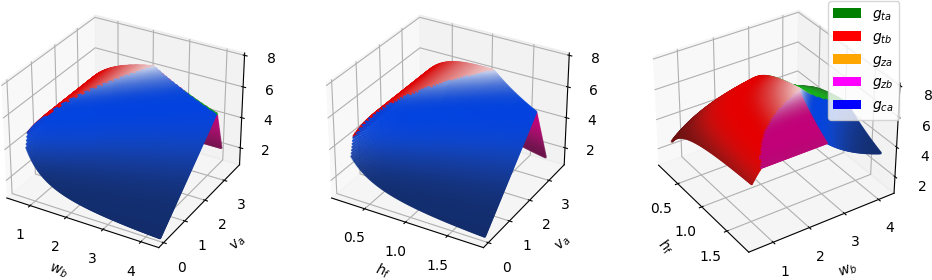
\includegraphics{sources-method-analytic_response_whole_bigger_fonts.png}
		\caption{Straight ITI\revise{M}{L} model response. At $\hf = 1.29$, $\wb=2.64$ and $\va=2.70$ respectively.}
		\label{interlocking:fig:analytic_response_whole}
	\end{subfigure}
	\begin{subfigure}[B]{\columnwidth}
		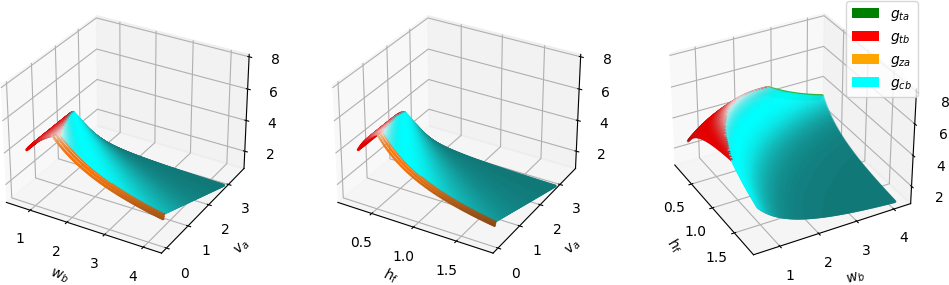
\includegraphics{sources-method-analytic_response_broken_bigger_fonts.png}
		\caption{Straight ITI\revise{M}{L} model response (broken). At $\hf = 0.50$, $\wb=1.50$ and $\va=0.36$ resp.}
		\label{interlocking:fig:analytic_response_broken}
	\end{subfigure}
	\caption{Maximum strength according to analytical models for the straight ITI\revise{M}{L} variant along three 2D slices of the 3D design space.
		Four constraint surfaces meet at the optimum.
		By taking the maximum values of these two models the maximum stress before separation can be calculated.
	}
	\label{interlocking:fig:analytic_response}
\end{figure}













\subsubsection{Broken cross beams model}
A careful analysis of the geometry will show that if shear failure $\mxz{a}$ has occurred, 
there is still interlocking between the two materials. 
If a part of the cross beams of $a$ has sheared off, still the pillar of material $a$ remains, which is surrounded by material $b$.
See \cref{interlocking:fig:straight_model_broken}.
Once failure mode $\mxz{a}$ has occurred, still any other failure mode has to occur for the interlock to fail completely.
Since the failure mode can only happen by part of the PP cross beam pushing against the part of the \revise{T}{}PLA cross beam which is being sheared off,
both cross beams shear together.
Because \revise{T}{}PLA breaks at a lower strain than PP (see \cref{interlocking:tab:mat_props_manufacturing_constraints}), we know that for these materials $\mxz{b}$ never occurs unless $\mxz{a}$ has occurred.
We will construct a separate model for analysing the case where the \revise{T}{}PLA cross beam is broken into segments.


Because part of the cross beam is missing the stress on the remaining part increases.
Moreover, the cross beam shear constraint for PP ($\gcbbroken$) comes into play and the Z shear constraint $\gzb$ and the cross beam shear constraint $\gca$ are dropped because of the change in the cross beam of $a$.
The shear constraints \crefrange{interlocking:eq:g_shear_a}{interlocking:eq:g_z_shear_b} are replaced by \cref{interlocking:eq:g_shear_b_broken,interlocking:eq:g_z_shear_a_broken}.

\begin{figure}
\begin{tcolorbox}[colback=white,title=Straight ITI\revise{M}{L} variant - shear constraints for broken case]
	\begin{align}
		\gcbbroken: & \frac{ F }{ 2 \left( \lmax - \va \right) 2 \hmin } \le  \frac{1}{\sqrt{3}} \sigmafail{b} &&	 \mxz{b}  \label{interlocking:eq:g_shear_b_broken} \\
		\gzabroken: & \frac{ F }{ 2 \va \wa } \le \frac{1}{\sqrt{3}} \sigmafailz{a}  	&&	 \mxy{a} \label{interlocking:eq:g_z_shear_a_broken}
	\end{align}
\end{tcolorbox}
\end{figure}
The response surface of this model is shown in \cref{interlocking:fig:analytic_response_broken}.
In order to estimate the ultimate force of a given design one must consider both of these models: the one for the whole and the one for the broken situation.
When considering designs where the cross beam constraint $\gca$ is active in the whole model, the maximal force applicable is the highest of the two maximal forces according to the two models.















\subsection{Diagonal ITI\revise{M}{L} variant}
Besides the straight variant of the ITI\revise{M}{L} lattice, we also consider the variant where the beams are oriented diagonally to the interface surface.
\Cref{interlocking:fig:diagonal_model_simple} shows a simple cell of the ITI\revise{M}{L} lattice in the diagonal orientation.
Because the stress applied is homogeneous and precisely normal to the interface the optimal structure should be symmetric.
Due to symmetry there is no distinction between fingers and cross beams to be made in this model.
Both beams should have the same height $2\hmin$ and the angle $\alpha$ between the beams and the interface of both beams is the same.
The remaining design variables are: $\wa$, $\wb$ and $L$.

The simple cell consists of protruding fingers and triangular dents (see red triangles in \cref{interlocking:fig:diagonal_model_simple});
however, the advantage these dents give to the strength of the pattern is vastly outweighed by their effect on the total length $L$.
We therefore trim the triangular ends on the pattern to arrive at the model shown in \cref{interlocking:fig:diagonal_model}.
However, doing this introduces some sharp edges, with a diameter below the minimum feature size $\wmin{}$.
We therefore round the vertical edges using a radius $r=\SI{0.15}{\milli\meter}$
and define the dimensions of the model such that the rounded edges at the ends of both fingers are aligned.
See \cref{interlocking:fig:analytical_math_diagonal}.


Because of the diagonal geometry we expect that the stress distribution throughout the structure will be quite complex,
and the failure will depend on the deformation of both materials during stretching.
Nevertheless, we provide a simplified analytical model assuming the stress is homogeneously distributed and disregarding the influence of deformation on stress distribution.
We decompose the force $F$ into one component parallel and another orthogonal to the direction of the beams.
We then use the parallel component to determine the tensile stress and the orthogonal component to determine the shear stress in the beam,
which combine into a single constraint using the von Mises yield criterion in \cref{interlocking:eq:g_tensile_m_diag}.
The diagonal ITI\revise{M}{L} model is then defined by the constrained optimization problem given by \crefrange{interlocking:eq:objective_diagonal}{interlocking:eq:g_z_shear_m_diag}.



\begin{figure}
	\begin{tcolorbox}[colback=white,title=Model for the diagonal ITI\revise{M}{L} variant]
	\begin{align}
		f: & \max{ \frac{F}{ 2h d } }  \label{interlocking:eq:objective_diagonal} \\
		\omit\rlap{subject to} \nonumber \\
		\gwa: & \wa \ge 2\wmin{a}		&&	\label{interlocking:eq:gwa_diag}\\
		\gwb: & \wb \ge 2\wmin{b}		&&	\label{interlocking:eq:gwb_diag}\\
		\gd:  & L \le \lmax && \label{interlocking:eq:gd_diag}\\
		\gtm: & \frac{ F }{ 2 \wm h } \sqrt{ \left( \frac{w}{d} \right)^2  + 3 \left( \frac{w}{2M} \right)^2 } \le \sigmafail{m} &&	\mt{m}  \label{interlocking:eq:g_tensile_m_diag} \\
		%\gtb: & \frac{ F }{ 2 \wb h } \sqrt{ \left( \left( \frac{w}{d} \right)^2  + 3 \left( \frac{d}{2M} \right)^2 \right) } \le \sigmafail{b} &&	\mt{b}  \label{interlocking:eq:g_tensile_b_diag} \\
		%\gtb: & \frac{ F }{ 2 \wb h } \sqrt{ \left( \left( \frac{w}{d} \right)^2  + 3 \left( \frac{d}{2M} \right)^2 \right) } \le \sigmafail{b} &&	\mt{b}  \label{interlocking:eq:g_tensile_b_diag} \\
		\gzm: & \frac{F}{2 A_{\text{z},m}} \le  \frac{1}{\sqrt{3}} \sigmafailz{m} 	&&	 \mxy{m} \label{interlocking:eq:g_z_shear_m_diag} \\
		%\gza: & \frac{F}{2 A_{\text{z},a}} \le \sigmafailz{a} 	&&	 \mxy{a} \label{interlocking:eq:g_z_shear_a_diag} \\
		%\gzb: & \frac{F}{2 A_{\text{z},b}} \le \sigmafailz{b} 	&&	 \mxy{b} \label{interlocking:eq:g_z_shear_b_diag} \\
		\omit\rlap{where} \nonumber \\
		d &= 2Mw / \sqrt{4M^2-w^2} \nonumber \\
		M &= L - 2r \nonumber \\
		w &= \wa + \wb \nonumber \\
		A_{\text{z},m} &= 	\rlap{$\frac12 \pi r^2 + r (\wm-2r) \frac{d}{w} + d M \left(\frac{\wm}{w}\right)^2$} \nonumber \\
		\omit\rlap{where \cref{interlocking:eq:g_z_shear_m_diag,interlocking:eq:g_tensile_m_diag} are duplicated  } \nonumber \\ 
		\omit\rlap{for both materials $ m \in \left\{a, b\right\} $ } \nonumber
	\end{align}
\end{tcolorbox}
\end{figure}




\iffalse
area of \revise{T}{}PLA under shear and tension: $\wa h$.
von Mises criterion:
\begin{align*}
	\left( \frac{ \nicefrac12 \nicefrac{w}{d} F }{ \wa h } \right)^2 + 3 \left( \frac{ \nicefrac12 \nicefrac{d}{2M} F }{ \wa h } \right)^2 &\le \sigmafail{a}^2 \\
	\left( \frac{ F }{ 2 \wa h } \right)^2 \left( \left( \frac{w}{d} \right)^2  + 3 \left( \frac{d}{2M} \right)^2 \right) &\le \sigmafail{a}^2 \\
	\frac{ F }{ 2 \wa h } \sqrt{ \left( \left( \frac{w}{d} \right)^2  + 3 \left( \frac{d}{2M} \right)^2 \right) } &\le \sigmafail{a} \\
	F \sqrt{ \left( \left( \frac{w}{d} \right)^2  + 3 \left( \frac{d}{2M} \right)^2 \right) } &\le 2 \sigmafail{a} \wa h \\
	F &\le \frac{ 2 \sigmafail{a} \wa h }{  \sqrt{ \left( \frac{w}{d} \right)^2  + 3 \left( \frac{d}{2M} \right)^2 } }  \\
\end{align*}


% NAIVE pp stress: area of PP under tension alone $\mt{b}$: $ 2h \frac{\wb}{w} d$. PP tensile stress: $\frac{\nicefrac12 F w}{\wb d 2 h} = \frac{F w}{4 \wb d h} \le \sigmafail{b}$
\fi


Again the stresses are all scale-invariant, so we set $\wa = 2 \wmin{a}$.
However, because changes in $\wb$ given the same $L$ will change the angle $\alpha$ of the beams, we cannot assume the design constraint $\gd$ is active.

The resulting response surface can be viewed in \cref{interlocking:fig:analytic_response_diagonal}.
Because the height of the fingers is minimal the Z shear constraints are both dominated.


\begin{figure}
	\centering
	\begin{subfigure}[B]{.4\columnwidth}
		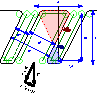
\includegraphics{sources-method-diagonal_math.pdf}
		\caption{Geometric relations.}
		\label{interlocking:fig:analytical_math_diagonal}
	\end{subfigure}
	\begin{subfigure}[B]{.59\columnwidth}
		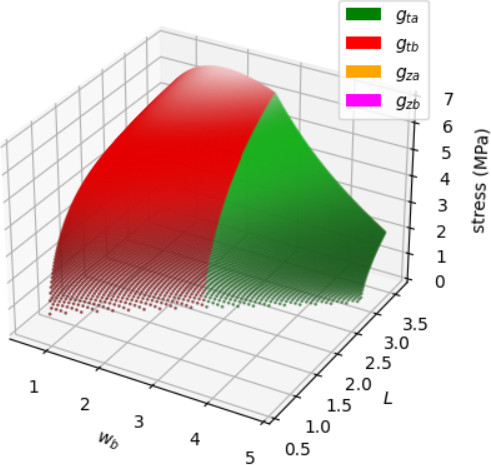
\includegraphics{sources-method-analytic_response_diagonal.jpg}
		\caption{Response surface coloured to failure mode.}
		\label{interlocking:fig:analytic_response_diagonal}
	\end{subfigure}
	\caption{Analytical model for the diagonal ITI\revise{M}{L} cell. The Z shear constraints are redundant because of the small height of the unit cell. The optimum is determined only by the tensile constraint of PP: $\gtb$.}
	%	\label{interlocking:fig:analytic_response}
\end{figure}




% !TeX spellcheck = en_US 
\section{Validation}\label{interlocking:sec:validation}
In order to validate our analytical models we compare its predictions against both simulation results and physical tensile tests.
While the physical tests constitute the final arbiter on the matter,
our resources for performing physical tests are limited.
Simulations can easily be performed by running a script for multiple days without user interaction.
Given that the simulations make use of the same material properties which were acquired from tensile tests performed by Ultimaker,
the simulations can teach us about the validity of the homogeneity assumptions in the analytical models.
Moreover, the physical test results are afflicted with a spread in manufacturing inaccuracies.
The simulations can therefore enrich the understanding we gain from physical experiments.




% !TeX spellcheck = en_GB 
\subsection{Simulation}
In order to simulate interlocking structures with a range of design parameters we automatically generate an INP file in Abaqus CAE (2020) using a script.
Solving the INP file gives us the force-displacement graph, from which we can determine the ultimate tensile strength.
In order to simulate accurately we used the stress-strain curves from tensile tests on the base materials printed flat on the build plate as the plasticity in tabular form.
The simulations were performed in the Abaqus/Explicit solver where Dynamic, Explicit procedure step was used with the mass scaling factor of $10^7$,
using geometric nonlinearity and general contact (explicit) to disregard friction for simplicity.

The repeating nature of the interlocking patterns was captured by modelling half of the unit cell and apply symmetry constraints to the sides, top and bottom.
The model was meshed using C3D8R hexahedral elements of $\pm\SI{75}{\micro\meter}$.

A grid search was used to measure the influence on the ultimate strength along each of the design variables $\wb (,\va, \hc)$, along with the total length $L$.
The search space was therefore 4D and 2D for the straight and diagonal design respectively.
In order to estimate the optimum we fit a smooth response surface to these data points using a radial basis function (RBF) network\cite{Dinh2002},
where a smoothness of $\lambda=1$ produces satisfactory results.


\subsubsection{Straight}
In order to prevent stress concentrations and adhere to manufacturing accuracy, the vertical edges of the straight design were rounded with $r=\SI{0.15}{\milli\meter}$;
see \cref{fig:sim_straight_model}.
We performed two rounds of hypersurface fitting on grid search; the second round was in a zoomed in region and with elements of $\pm\SI{50}{\micro\meter}$.

Newton's method was used to determine the optimum, starting from the best sampled point.
This step only considered the dimensions $\wb$ and $\va$, because $\lmax$ is given and $\hf$ has to be an integer multiple of $\hmin$.
It's unlikely the optimum of the fitted hypersurface would be on a different integer multiple of $\hmin$.
The resulting hypersurfaces are visualized in \cref{fig:simulation_results_straight}.
The obtained optima are shown in \cref{tab:sim_straight_optima}.

We compare the results of round 1 to our analytical model by adjusting the analytical model to capture the inaccurate Z strength used in the simulations:
$\sigmafailz{m} := \sigmafail{m}$.
See \cref{fig:ana_sim_accuracy_straight}.
We then observe that our analytical model on average predicts only \SI{7.8}{\percent} higher ultimate strength values than then the FEM simulations, with a standard deviation of \SI{16.2}{\percent}.

\begin{figure}
	\centering
	\setlength{\figheight}{.32\columnwidth}
	\begin{subfigure}[B]{.6\columnwidth}
		\centering
		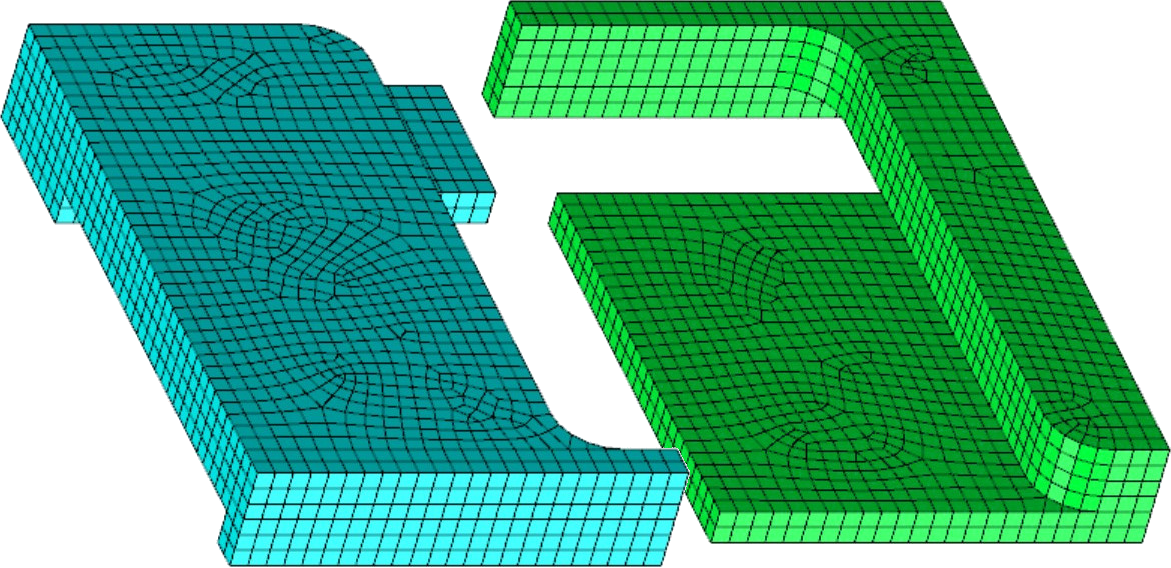
\includegraphics[height=\figheight]{sources/simulation/mesh-straight.png}
		\caption{Straight}
	\end{subfigure}
\hspace{-.5cm}
	\begin{subfigure}[B]{.39\columnwidth}
		\centering
		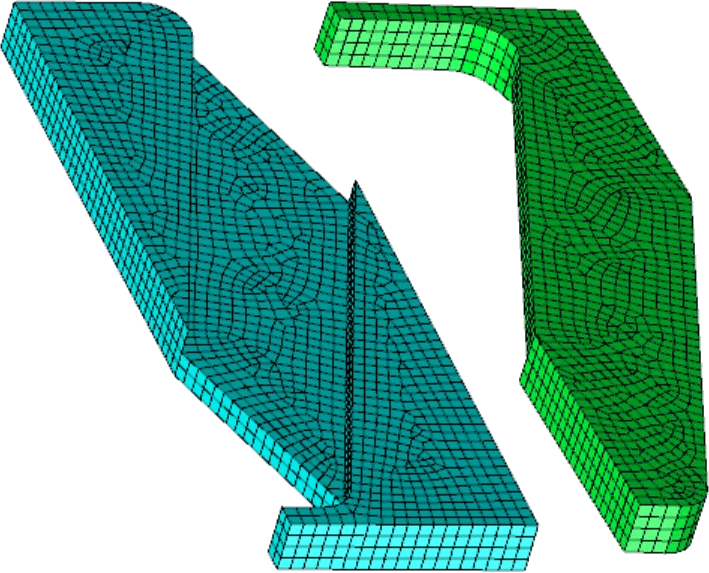
\includegraphics[height=\figheight]{sources/simulation/mesh-diagonal.png}
		\caption{Diagonal}
	\end{subfigure}
	\caption{Example simulation meshes. The diagonal mesh is half a unit cell.}
	\label{fig:sim_straight_model}
\end{figure}



\begin{figure*}
	\centering
	\begin{subfigure}[B]{.49\columnwidth}
		\centering
		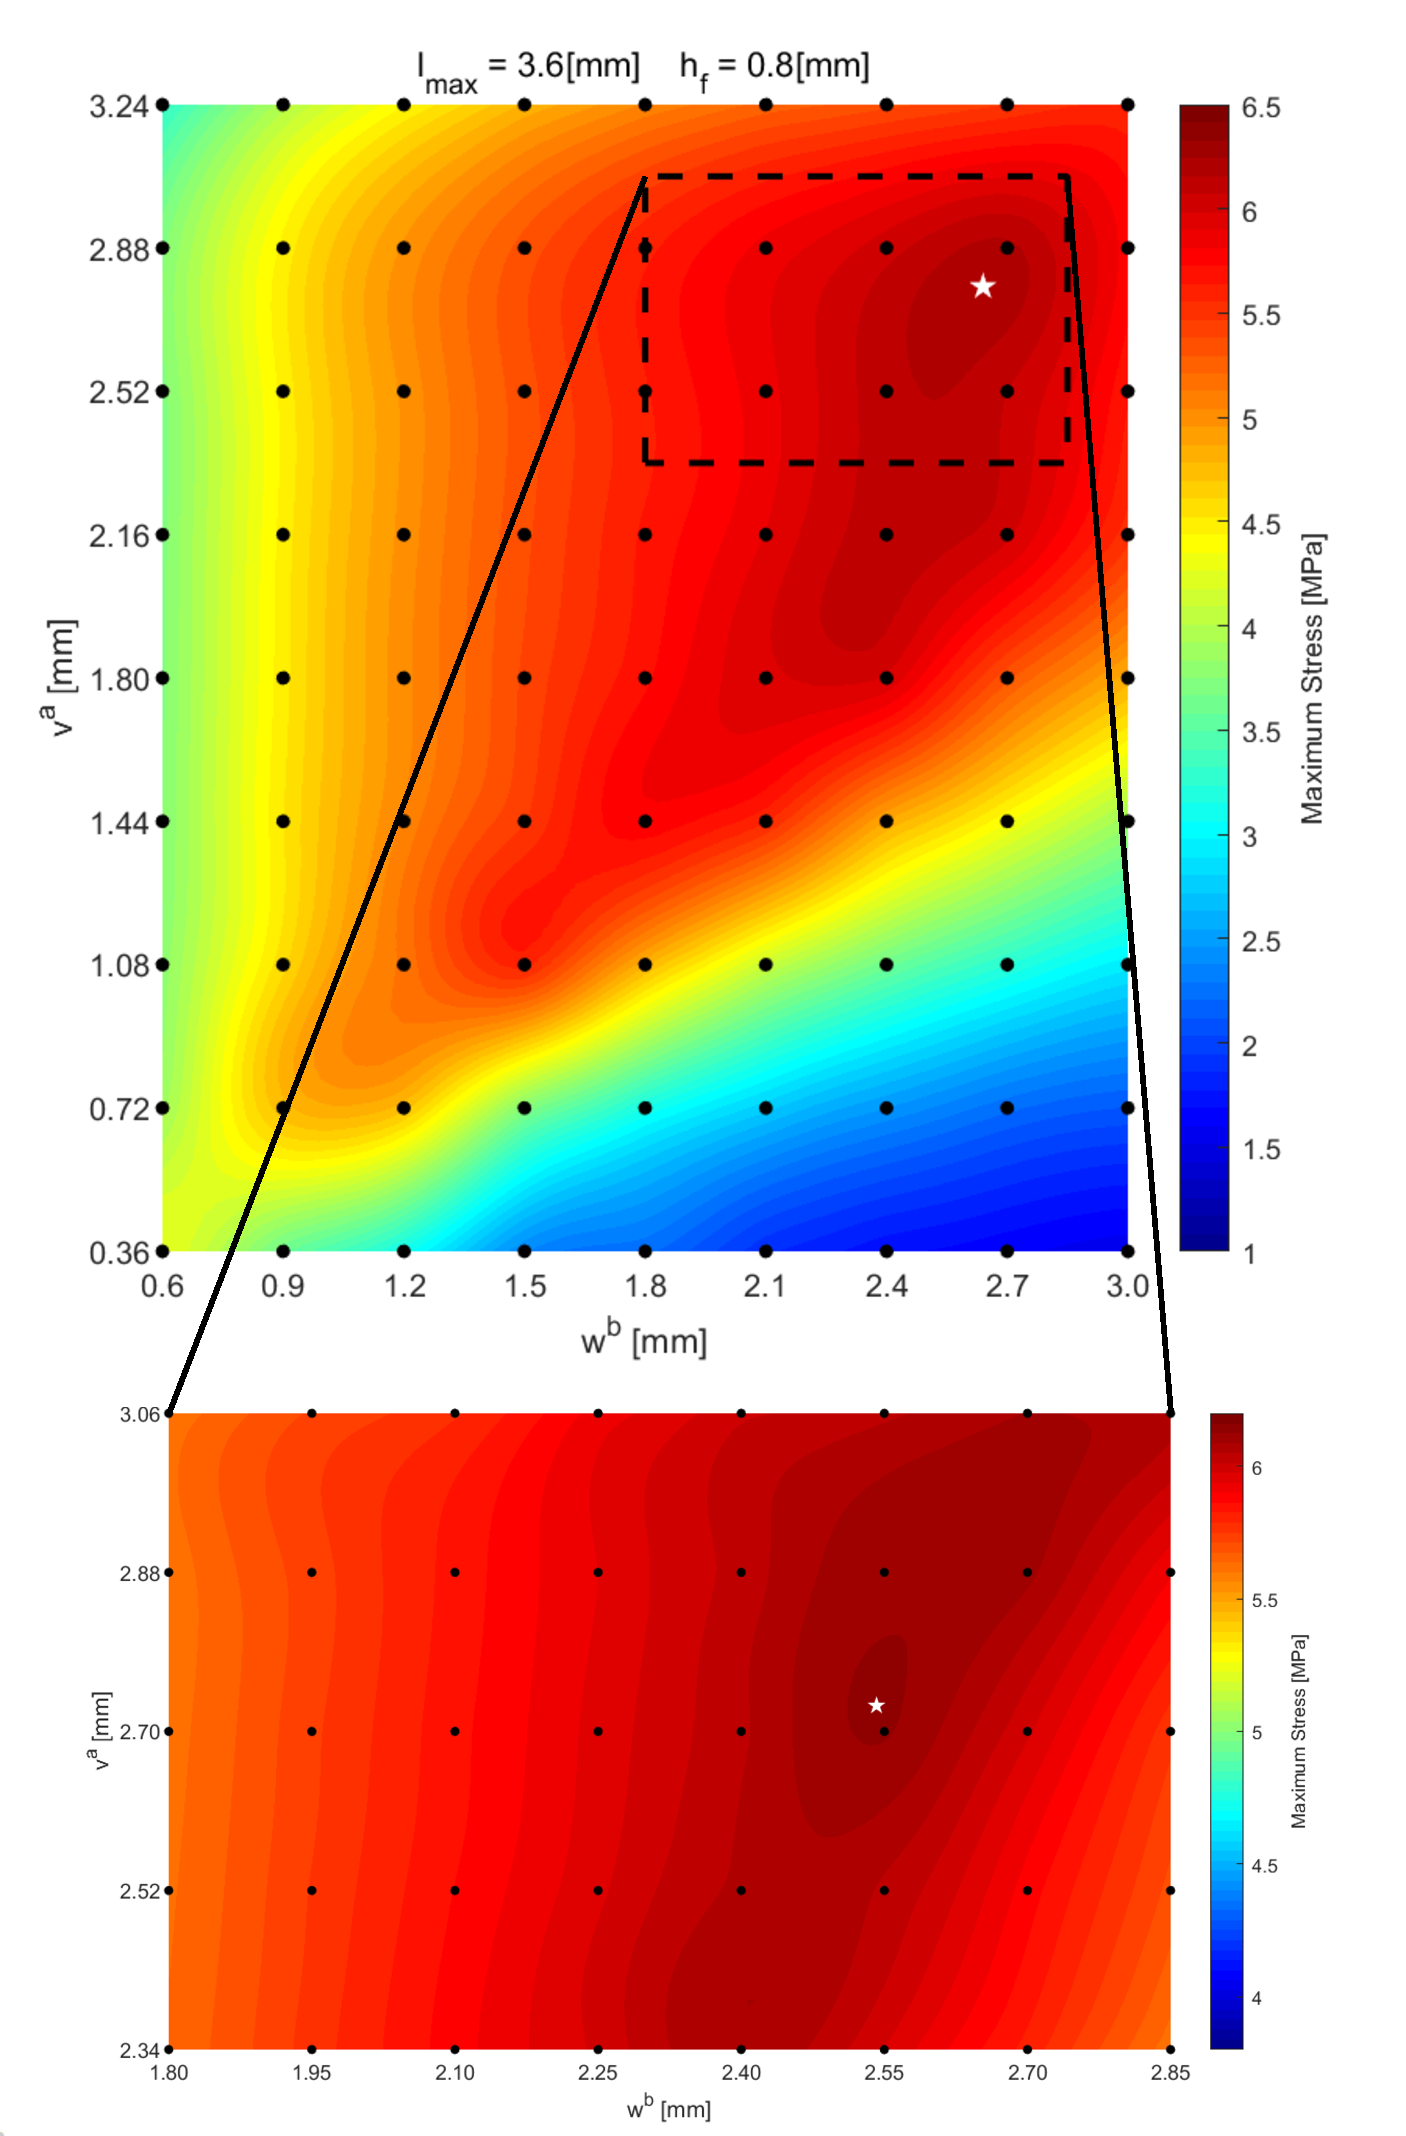
\includegraphics{sources/simulation/r12-lmax3.6.pdf}
		\caption{$\lmax=\SI{3.6}{\milli\meter}; \hf=\SI{0.8}{\milli\meter}$}
	\end{subfigure}
	\begin{subfigure}[B]{.49\columnwidth}
		\centering
		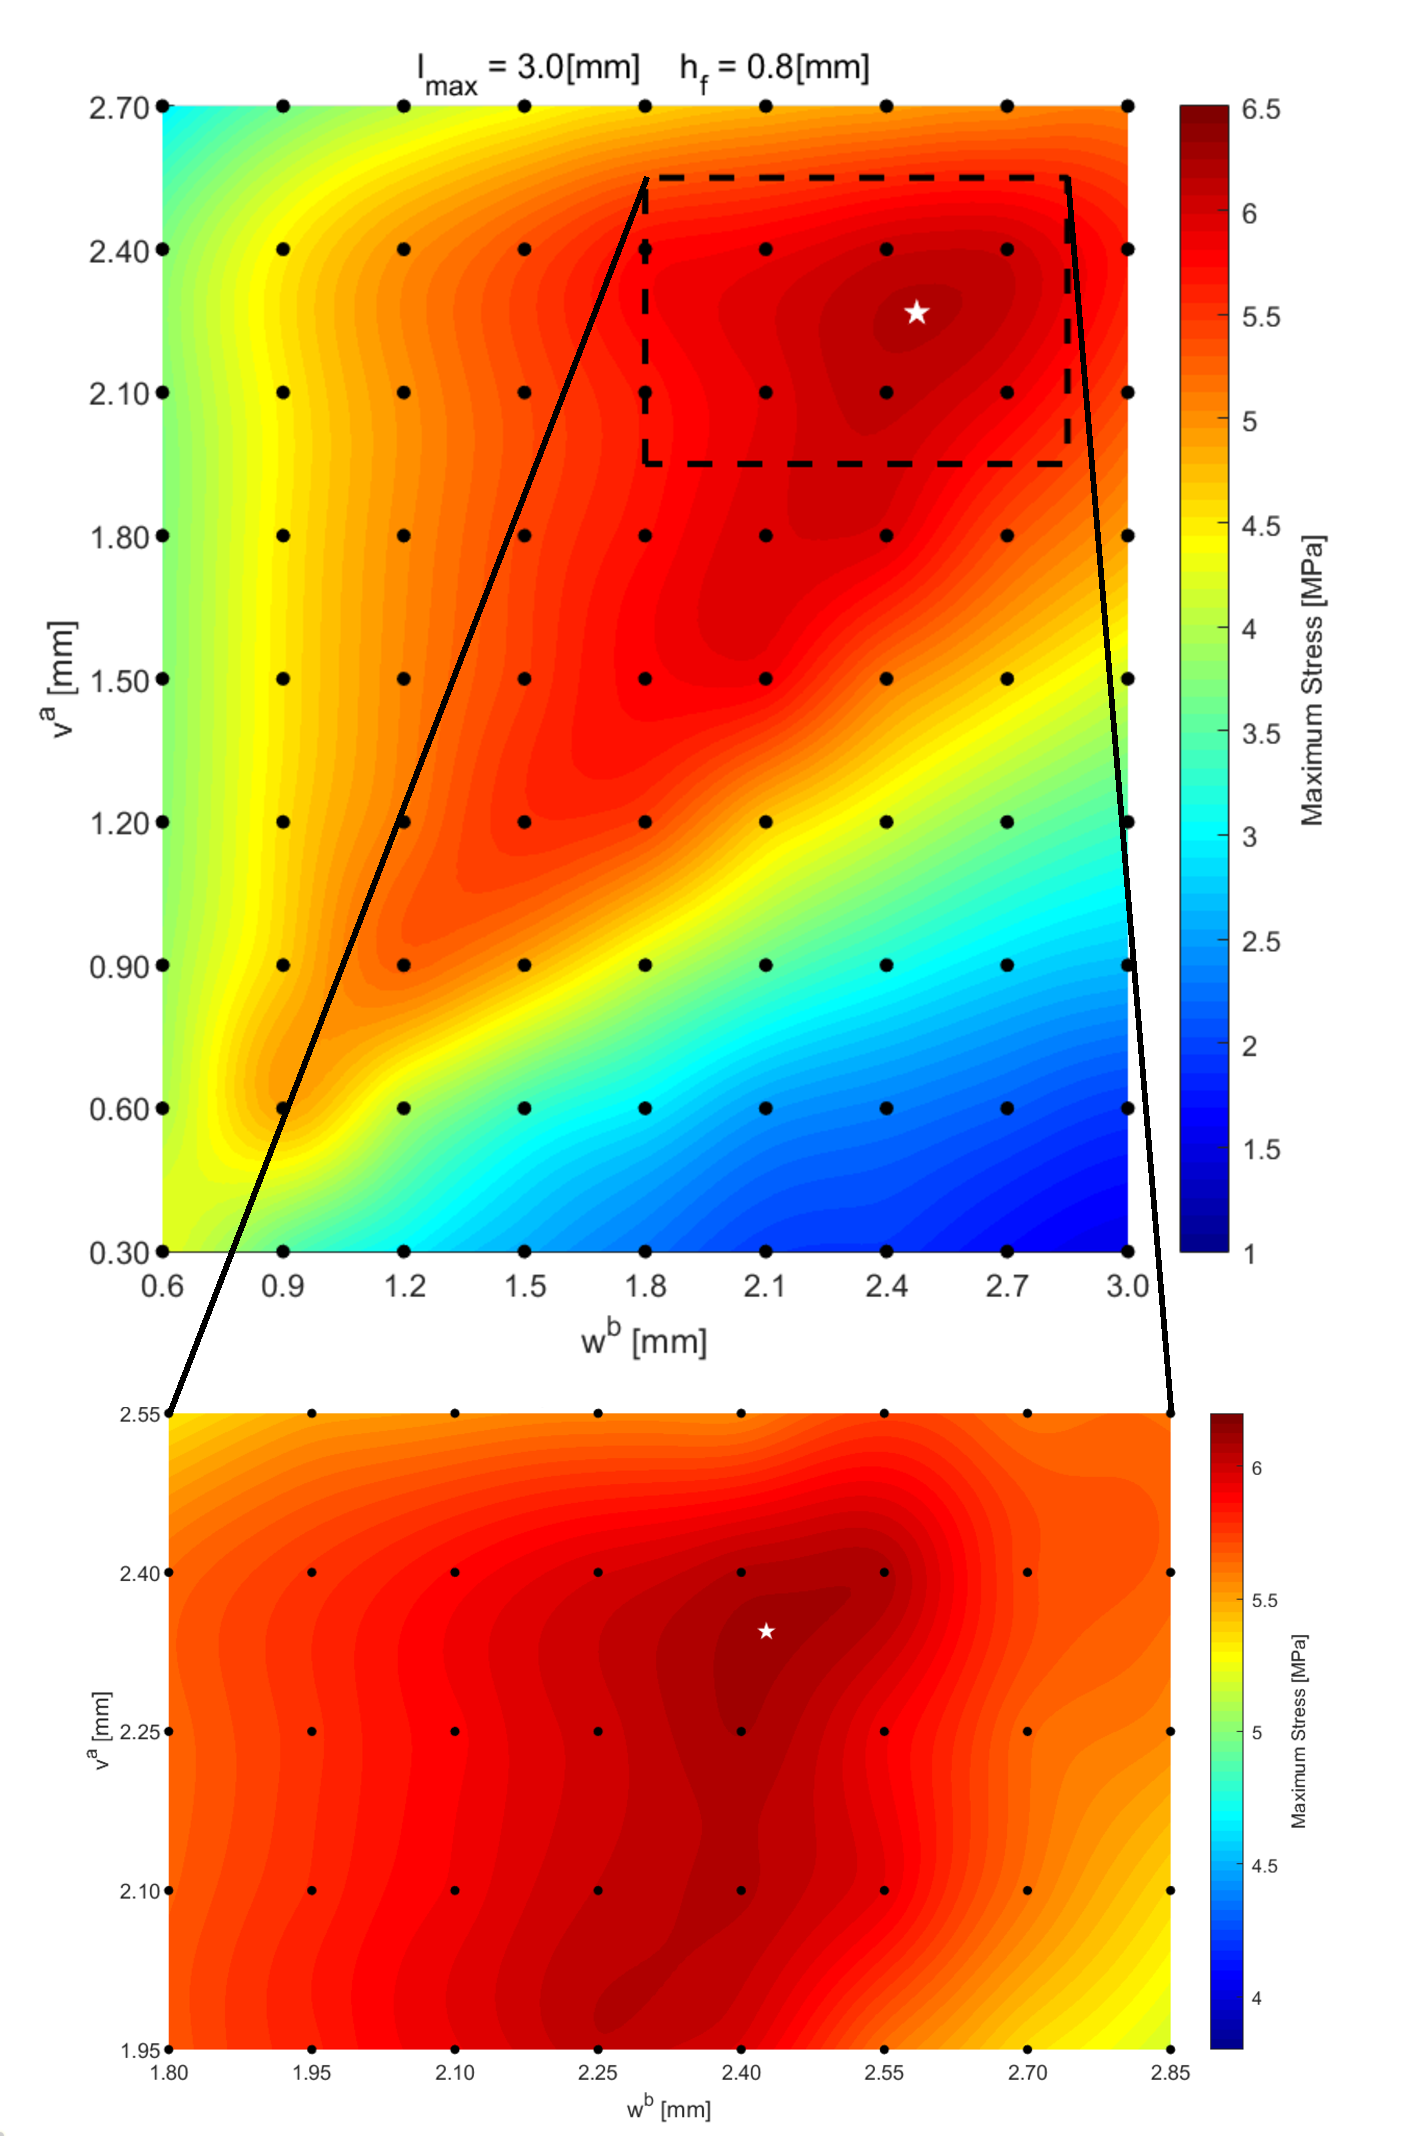
\includegraphics{sources/simulation/r12-lmax3.0.pdf}
		\caption{$\lmax=\SI{3.0}{\milli\meter}; \hf=\SI{0.8}{\milli\meter}$}
	\end{subfigure}
	\begin{subfigure}[B]{.49\columnwidth}
		\centering
		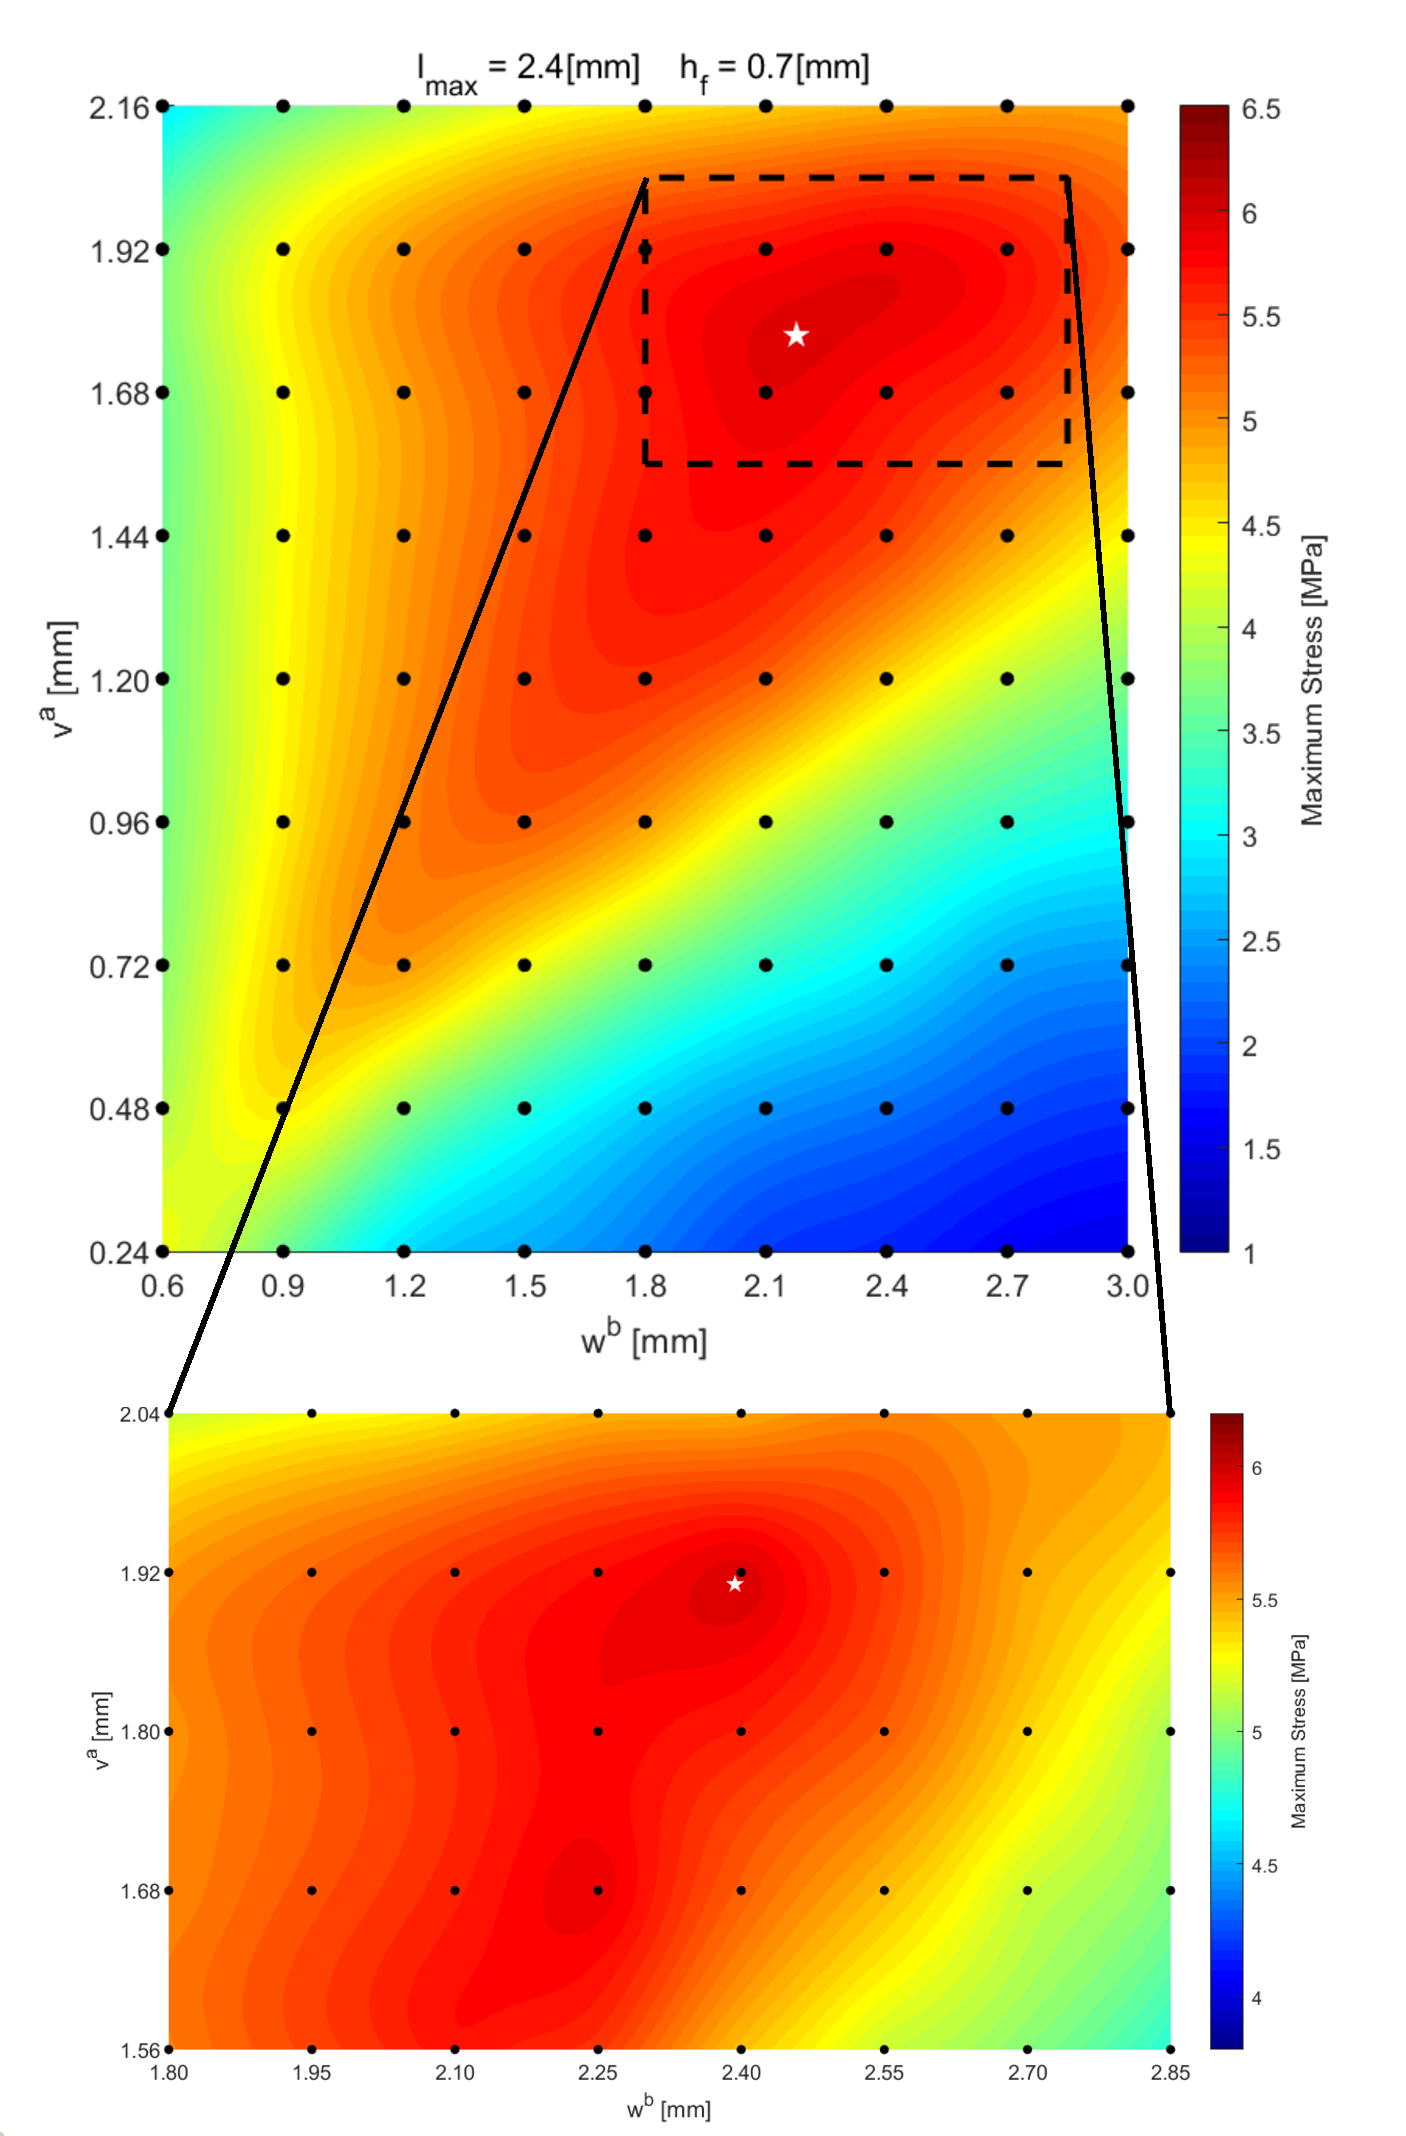
\includegraphics{sources/simulation/r12-lmax2.4.pdf}
		\caption{$\lmax=\SI{2.4}{\milli\meter}; \hf=\SI{0.7}{\milli\meter}$}
	\end{subfigure}
	\begin{subfigure}[B]{.49\columnwidth}
		\centering
		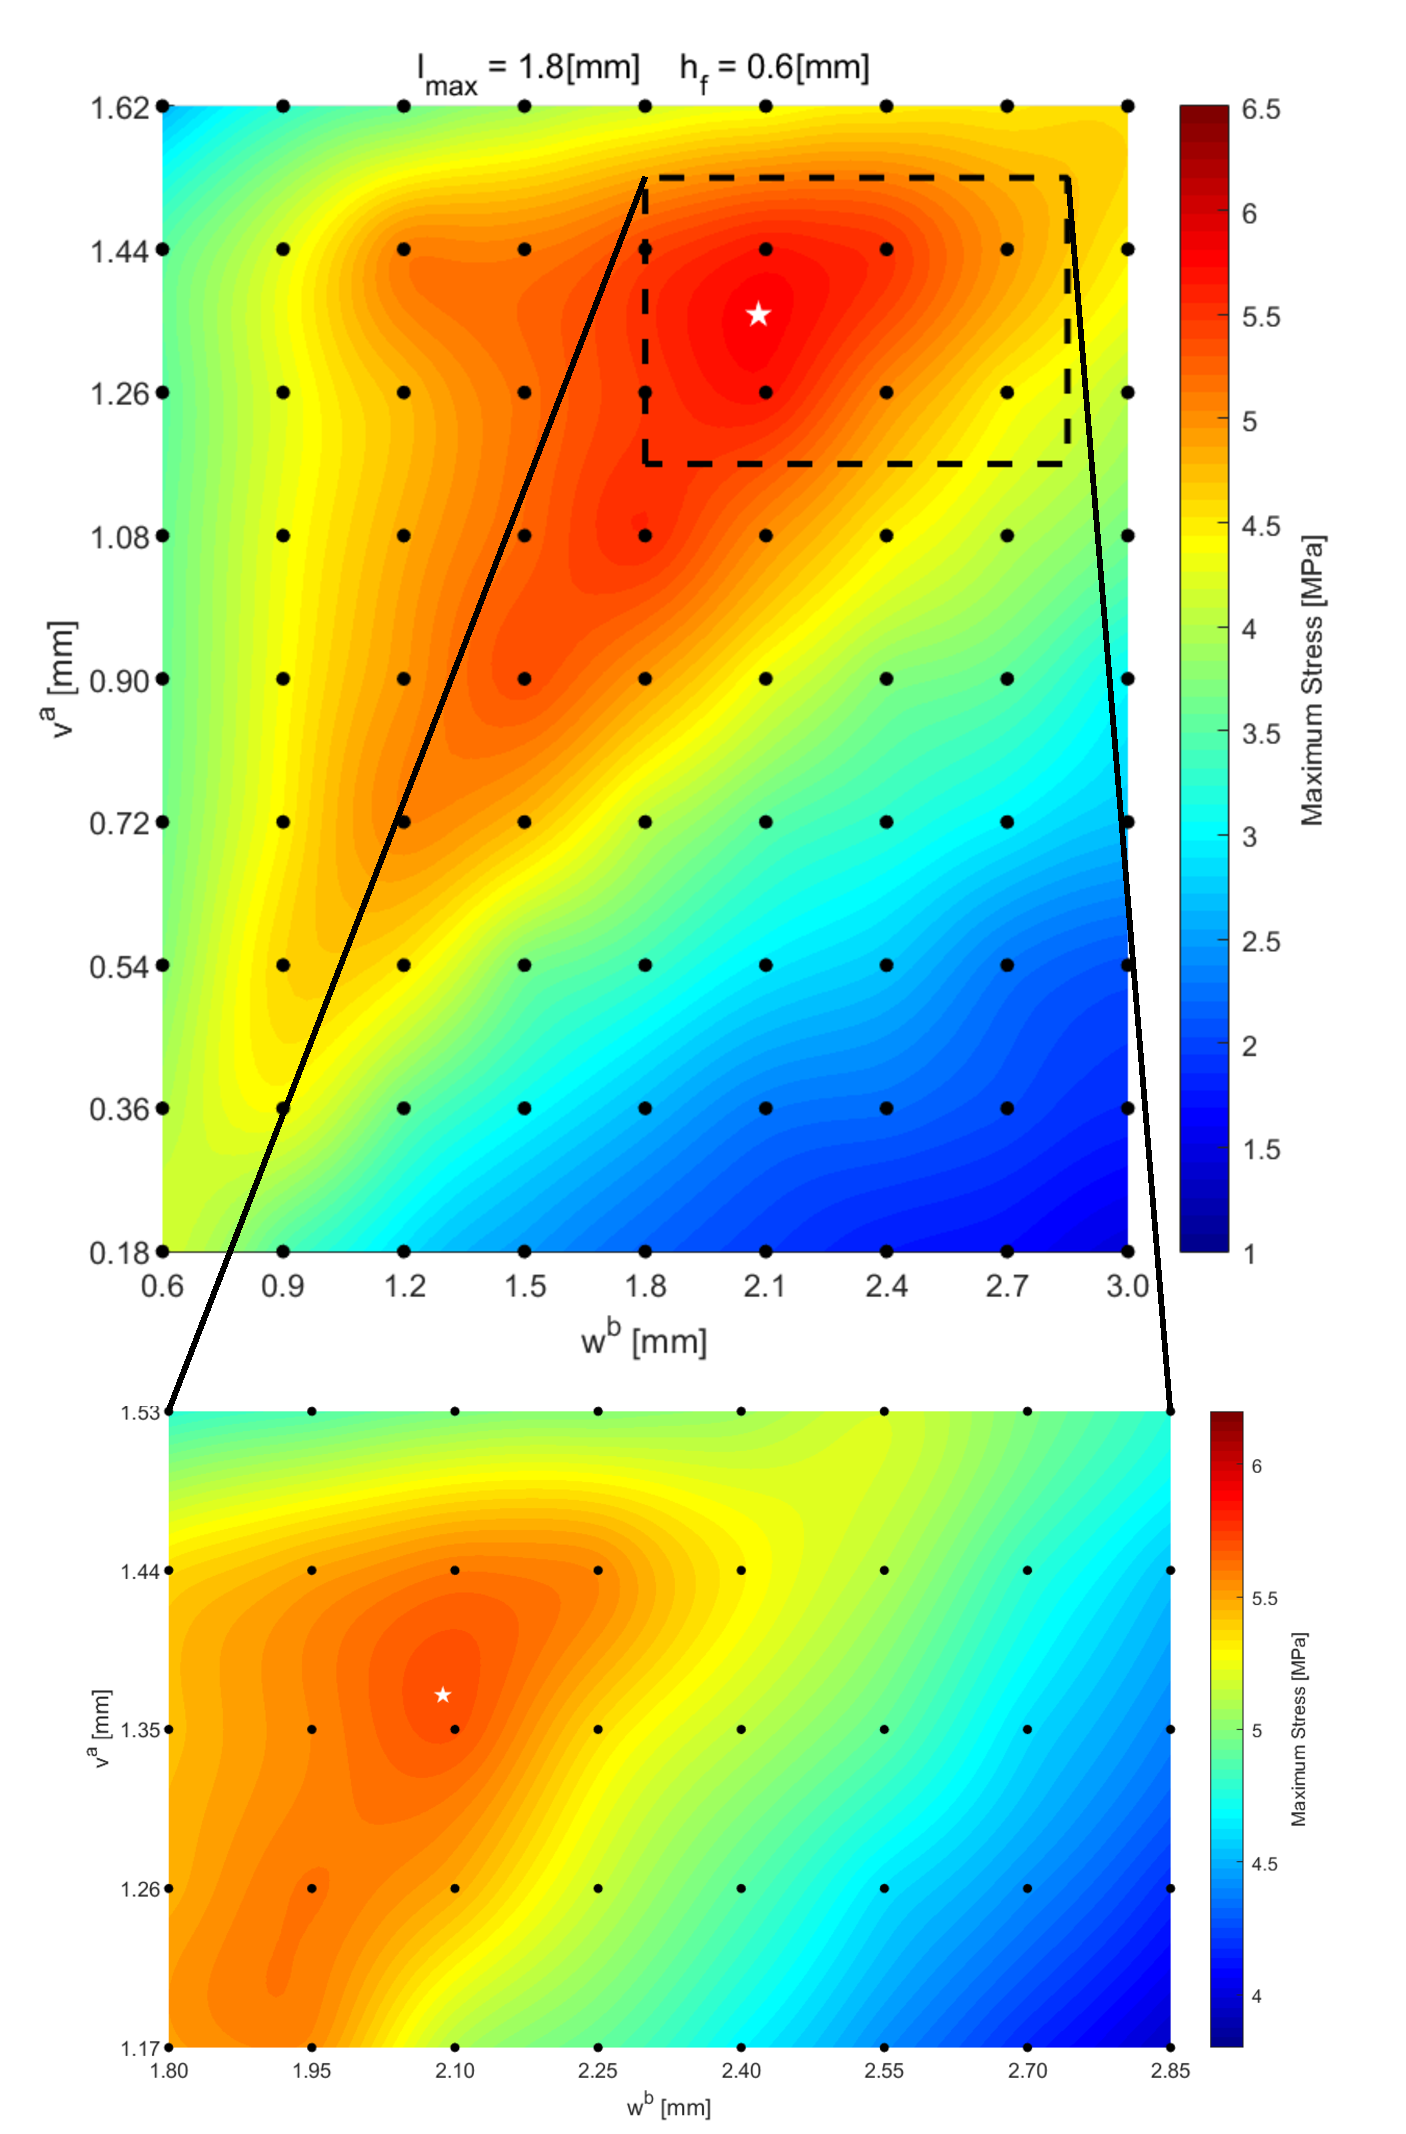
\includegraphics{sources/simulation/r12-lmax1.8.pdf}
		\caption{$\lmax=\SI{1.8}{\milli\meter}; \hf=\SI{0.6}{\milli\meter}$}
	\end{subfigure}
	\caption{2D slices of the 4D simulation results and fitted hypersurface for the straight design. Sampled data points in black, optimum in white.}
	\label{fig:simulation_results_straight}
\end{figure*}

\begin{table}
	\caption{Optimal designs according to the hypersurface fitted to the FEM simulations for the second round of the straight model and for the diagonal model.}
	\label{tab:sim_straight_optima}
	\begin{tabular}{ll|llll}
		&$\lmax$ (\si{\milli\meter})             & 3.6 & 3.0 & 2.4 & 1.8 \\
		\hline
		\multirow{4}{*}{\rotatebox[origin=c]{90}{straight}}
		&$\sigma_\text{max}$ (\si{\mega\pascal}) & \bf 6.11 & \bf 6.03 & \bf 5.81 & \bf 5.53 \\
		&$\hf$ (\si{\milli\meter})               & 0.8 & 0.8 & 0.7 & 0.6 \\
		&$\wb$ (\si{\milli\meter})               & 2.54 & 2.35 & 2.22 & 2.01 \\
		&$\va$ (\si{\milli\meter})               & 2.82 & 2.27 & 1.84 & 1.36 \\
		\hline
		\multirow{2}{*}{\rotatebox[origin=c]{90}{diag}}
		&$\sigma_\text{max}$ (\si{\mega\pascal}) & \bf 6.30 & \bf 6.37 & \bf 5.86 & \bf 4.69 \\
		&$\wb$ (\si{\milli\meter})               & 1.21 & 1.19 & 1.18 & 1.04 \\
		\end
		{tabular}
\iffalse
	\begin{tabular}{l|llllllll}
		Round & 1 & 2 & 1 & 2 & 1 & 2 & 1 & 2 \\
		\hline
		$\lmax$ (\si{\milli\meter}) & 3.6 & 3.6 & 3.0 & 3.0 & 2.4 & 2.4 & 1.8 & 1.8\\
		$\hf$ (\si{\milli\meter}) & 0.8 & 0.8 & 0.8 & 0.8 & 0.7 & 0.7 & 0.6 & 0.6 \\
		$\wb$ (\si{\milli\meter}) & 2.58 & 2.54 & 2.42 & 2.35 & 2.18 & 2.22 & 2.05 & 2.01\\
		$\va$ (\si{\milli\meter}) & 2.67 & 2.82 & 2.23 & 2.27 & 1.78 & 1.84 & 1.35 & 1.36 \\
		$\sigma_\text{max}$ (\si{\mega\pascal}) & 6.17 & 6.11 & 6.12 & 6.03 & 5.89 & 5.81 & 5.59 & 5.53
	\end{tabular}
\fi
\end{table}





\subsubsection{Diagonal}
Modelling the diagonal design in Abaqus can be quite cumbersome, since it doesn't natively support periodic boundary constraints.
Whereas this problem can be overcame in the straight design because it is symmetric,
the diagonal design is rotationally symmetric.
While a symmetry constraint can be used on the top and bottom, the two sides of the design are mirror images of each other, but also flipped vertically.

However, since the height of the beams is relatively low compared to their width we have observed that the stresses and strains are quite similar in the top and bottom.
If we model half of the diagonal cell by cutting it vertically and apply symmetry constraints to the sides,
the induced error is only approximately 10\% compared to simulating an interface consisting of two whole cells.
% small discontinuities



\begin{figure}
	\centering
	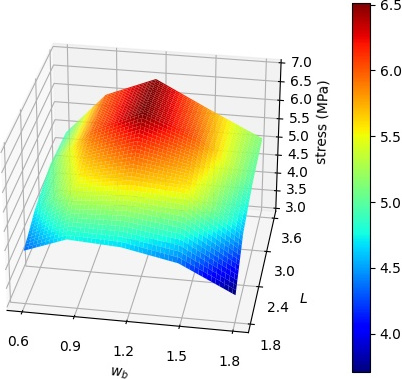
\includegraphics[width=.7\columnwidth]{sources/simulation/diagonal_sim_response.jpg}
	\caption{Diagonal results using linear interpolation between the simulation results.}
	\label{fig:sim_diagonal_model}
\end{figure}


The results of these simulations are shows in \cref{fig:sim_diagonal_model}.
The predictions from the analytical model can directly be compared to the simulation results, because the constraints on Z shear are not active.
See \cref{fig:ana_sim_accuracy_diagonal}.
The analytical model predicts only 0.4\% lower ultimate strength values on average with a standard deviation of 10\%.

%optimal designs table



\begin{figure*}
	\centering
	\setlength{\figheight}{.2\textwidth}
	\begin{subfigure}[B]{.7\textwidth}
		\centering
		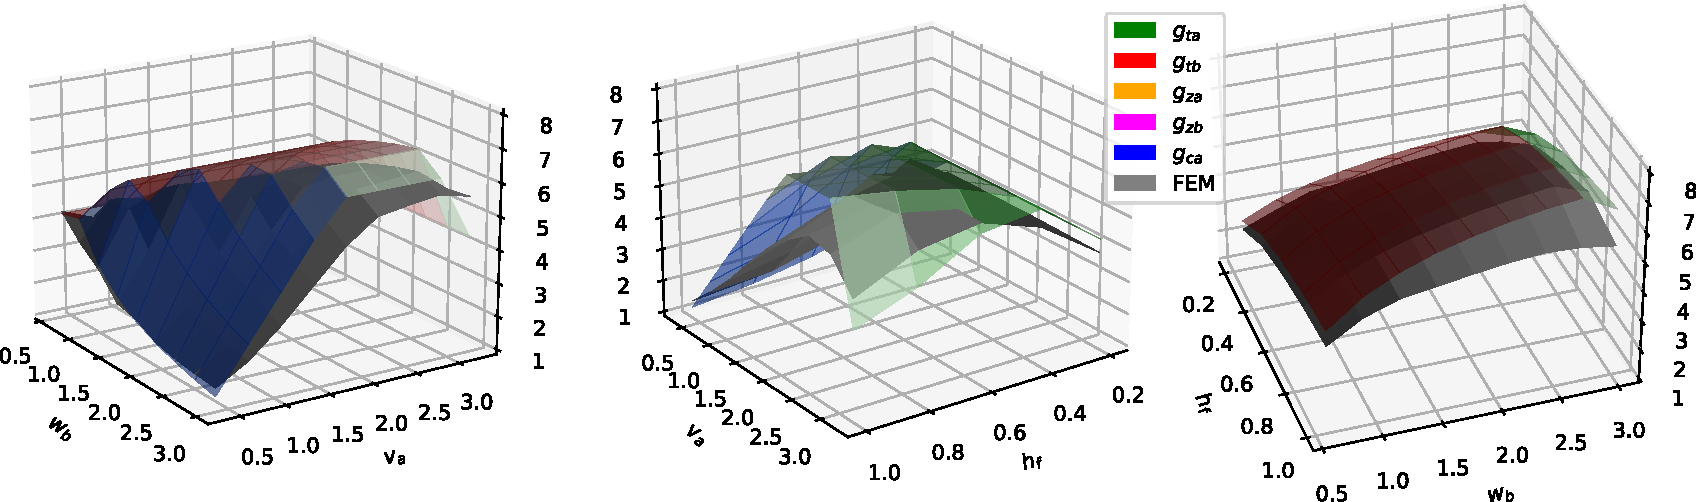
\includegraphics[height=\figheight]{sources/simulation/model_accuracy.pdf}
		\caption{Straight ITIM for $L=\SI{3.6}{\milli\meter}$}
		\label{fig:ana_sim_accuracy_straight}
	\end{subfigure}
	\hspace{-.5cm}
	\begin{subfigure}[B]{.29\textwidth}
		\centering
		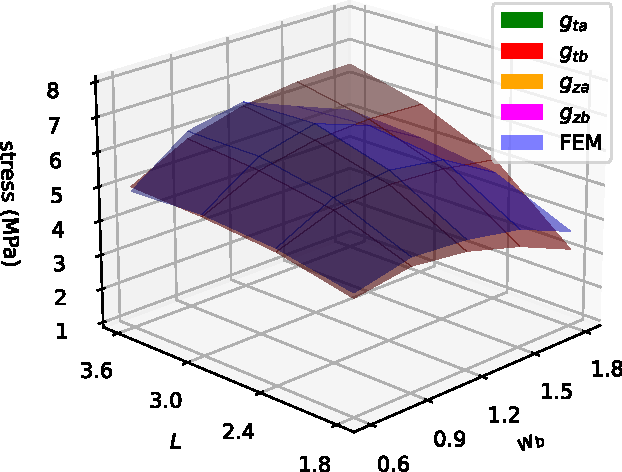
\includegraphics[height=\figheight]{sources/simulation/model_accuracy_diagonal.pdf}
		\caption{Diagonal ITIM for various values of $L$}
		\label{fig:ana_sim_accuracy_diagonal}
	\end{subfigure}
	\caption{Ultimate strength according to the analytical models and the simulation results. The analytical models follow roughly the same shape and same height as the simulation results. }
	\label{fig:ana_sim_accuracy}
\end{figure*}









\subsection{Physical experimental tests}
Tensile tests were performed on an Instron 3366 Universal Testing machine at \SI{5}{\milli\meter\per\minute}.
Prints were manufactured on a Ultimaker S5 systems in 5-fold with Ultimaker Green Tough PLA and Ultimaker PP using the default \SI{0.1}{\milli\meter} layer thickness profile,
with \SI{100}{\percent} infill and a custom brim to make sure both materials stick to the build plate.
For PP we print the outer before the inner walls so as to improve the dimensional accuracy. % on TPLA we forgot to edit those settings
In order to deal with the various widths of the beams we generate toolpaths using the Cura Arachne Engine beta release\cite{CuraArachne},
which implements a framework for generating variable line width toolpaths to fill small geometry of arbitrary dimensions\cite{Kuipers2020}.
The Inward Distributed and the Distributed strategy were used on TPLA and PP respectively.
See \cref{interlocking:fig:gcode}.



\begin{figure}
	\setlength{\figheight}{.42\columnwidth}
	\centering
	\begin{subfigure}[B]{.26\columnwidth}
		\centering
		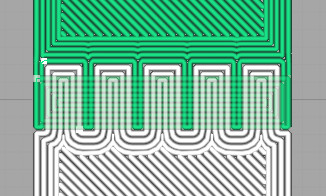
\includegraphics[width=\figheight,rotate=90]{sources-testing-straight_gcode.jpg}
		\caption{Straight ITIM}
		\label{interlocking:fig:gcode_straight}
	\end{subfigure}
	\begin{subfigure}[B]{.26\columnwidth}
		\centering
		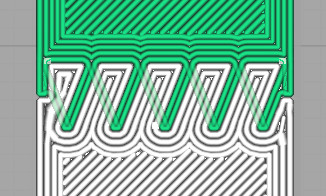
\includegraphics[width=\figheight,rotate=90]{sources-testing-diagonal_gcode.jpg}
		\caption{Diagonal ITIM}
		\label{interlocking:fig:gcode_diagonal}
	\end{subfigure}
	\begin{subfigure}[B]{.22\columnwidth}
		\centering
		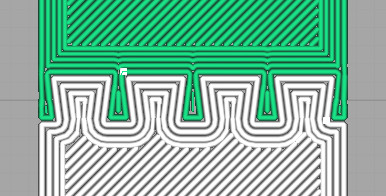
\includegraphics[width=\figheight,rotate=90]{sources-testing-suture_gcode.jpg}
		\caption{Trap. suture}
		\label{interlocking:fig:gcode_suture}
	\end{subfigure}
	\begin{subfigure}[B]{.22\columnwidth}
		\centering
		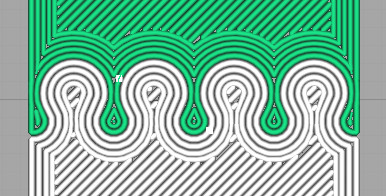
\includegraphics[width=\figheight,rotate=90]{sources-testing-jigsaw_gcode.jpg}
		\caption{Jigsaw}
		\label{interlocking:fig:gcode_jigsaw}
	\end{subfigure}
	\caption{Gcodes generated with Cura Arachne engine beta. The layers of main fingers are shown and the other layers in a transparent overlay. While the straight and diagonal ITIM lattice produce continuous extrusion beads, the toolpaths for the dovetail designs include small separated segments.}
	\label{interlocking:fig:gcode}
\end{figure}





\subsubsection{Model parameters}
\paragraph{Straight ITIM}
The straight ITIM variant suffers from the curse of dimensionality;
even when setting $\wa=\SI{0.6}{\milli\meter}$, $\hc=\SI{0.1}{\milli\meter}$ and $L=\SI{3.6}{\milli\meter}$,
there are still the three free design variables $\wb$, $\va$ and $\hf$ to determine.
With 5 specimens per sample point and limited resources, the total number of data points we are able to test is limited.
We therefore chose to sample close to the two optima of the analytical models: whole and broken, as well as deviations from those optima in both directions along the axis of each design variable of \SI{0.3}{\milli\meter} in $\wb$ and $\va$ and \SI{0.2}{\milli\meter} in $\hf$.
See \cref{interlocking:fig:test_points_straight}.

Each sample of the straight ITIM variant has $5\times5$ cells.
Because the repetition of cells is broken at the sides of the specimen, the boundary cells are adjusted for manufacturability and stability.
The specimens end with a TPLA finger on both sides and in cross beams on both top and bottom.
See \cref{interlocking:fig:test_straight_boundary_cells}.

\begin{figure}
	\centering
	\begin{subfigure}[B]{.24\columnwidth}
		\centering
		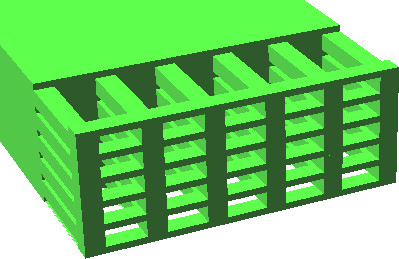
\includegraphics[width=\columnwidth]{sources-testing-straight_sample.jpg}
		\caption{Example print mesh near optimum}
		\label{interlocking:fig:test_straight_boundary_cells}
	\end{subfigure}
	\begin{subfigure}[B]{.24\columnwidth}
		\centering
		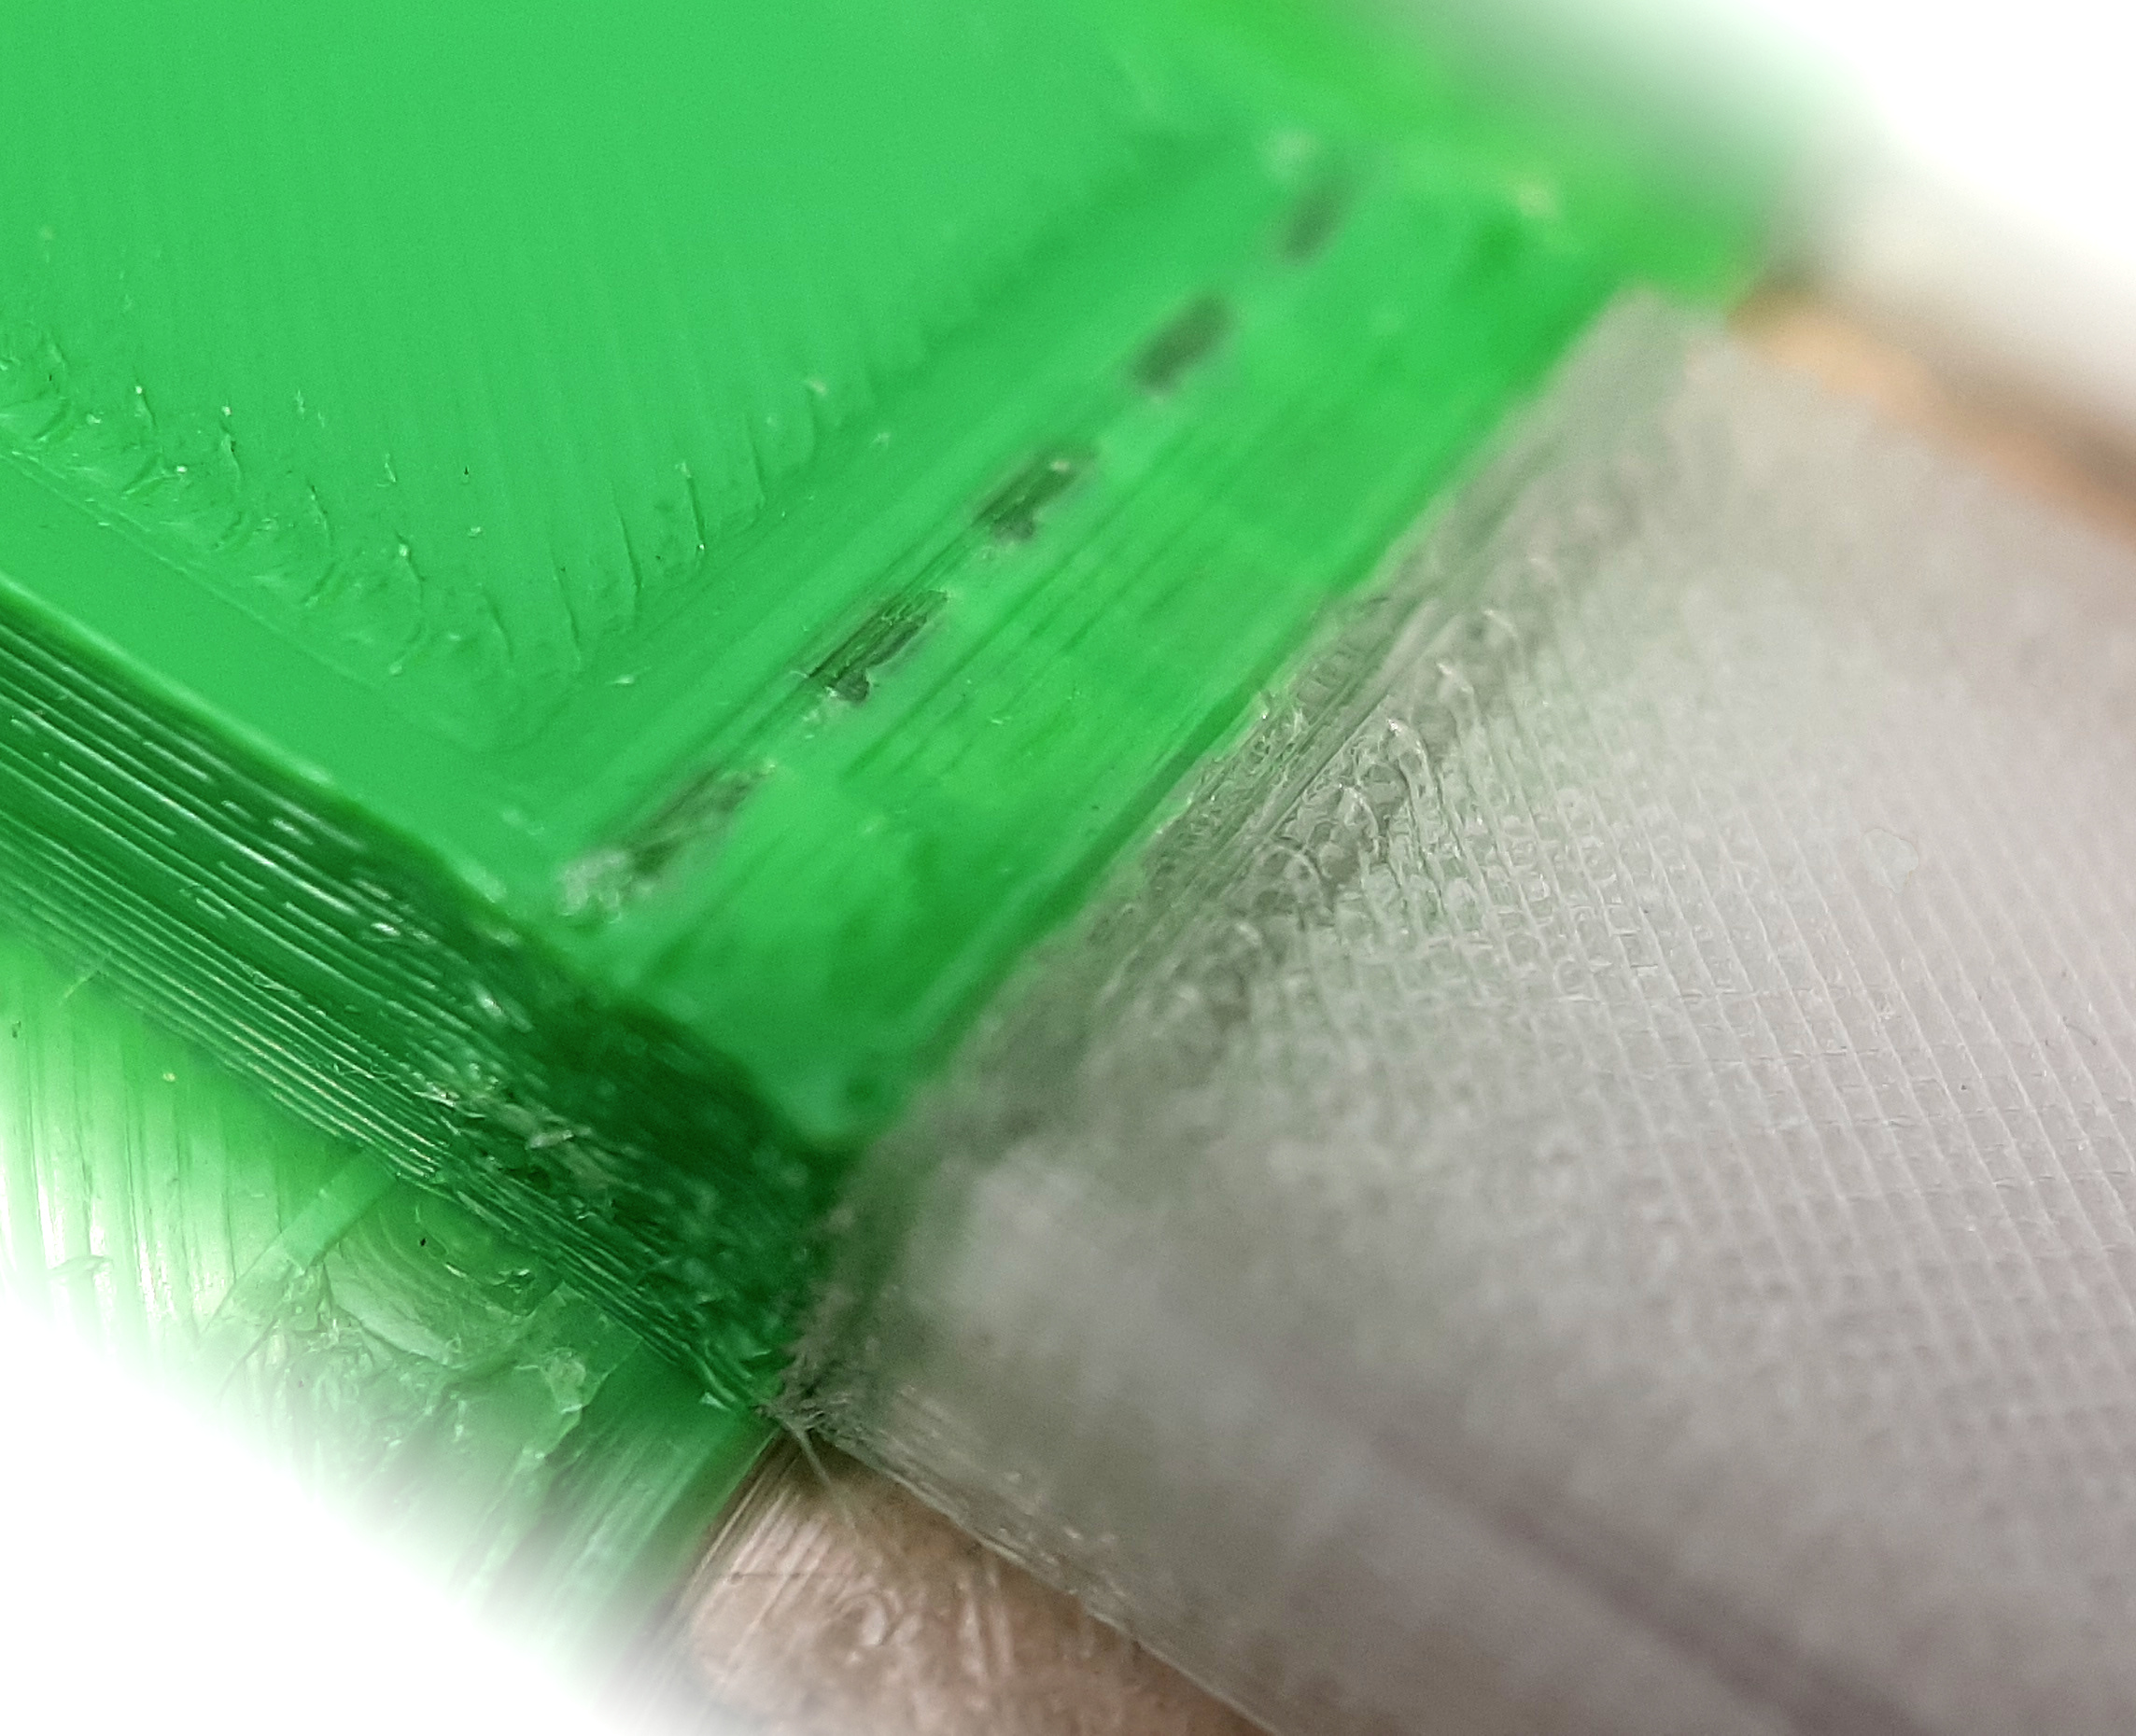
\includegraphics[width=\columnwidth]{sources-testing-straight_print.jpg}
		\caption{Example print near broken optimum}
	\end{subfigure}
	\begin{subfigure}[B]{.5\columnwidth}
		\centering
		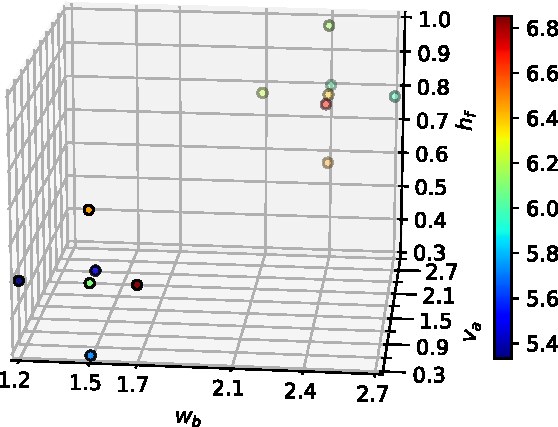
\includegraphics[width=\columnwidth]{sources-testing-straight_sample_points.pdf}
		\caption{Sampled points and measured cell stress.}
		\label{interlocking:fig:test_points_straight}
	\end{subfigure}
	\caption{Experimental setup of straight ITIM variant.
		Note that for the broken model $\va$ is minimal, so va- is not a valid sample.}
\end{figure}





\paragraph{Diagonal ITIM variant}
Each sample of the diagonal ITIM variant contains 5 cells in the horizontal direction, but 13 repetition in Z because of the low unit cell height.
Extra finger beams are added to the sides of the specimen to prevent any part of the beam to be less than $2\wmin=\SI{0.6}{\milli\meter}$ wide.
See \cref{interlocking:fig:gcode_diagonal}.
Because with a given $L=\SI{3.6}{\milli\meter}$, $h=\SI{0.2}{\milli\meter}$ and $\wa=\SI{0.6}{\milli\meter}$ the remaining design space is only one-dimensional,
we can simply sample various points along $\wb$: $(0.6, 1.2, 1.8, 2.4, 3.0, 3.6)$.

\iffalse
\begin{figure}
	\centering
	\begin{subfigure}[B]{.24\columnwidth}
		\centering
		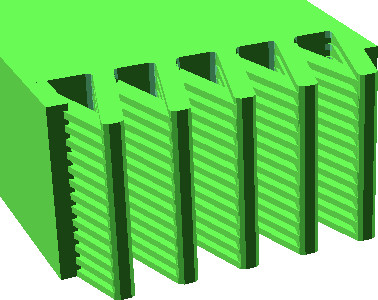
\includegraphics[width=\columnwidth]{sources-testing-diagonal_sample.jpg}
		\caption{Example print mesh}
		\label{interlocking:fig:test_diagonal_boundary_cells}
	\end{subfigure}
	\begin{subfigure}[B]{.24\columnwidth}
		\centering
		\includegraphics[width=\columnwidth]{sources-testing-diagonal_print.jpg}
		\caption{Example print}
	\end{subfigure}
	\begin{subfigure}[B]{.5\columnwidth}
		\centering
		%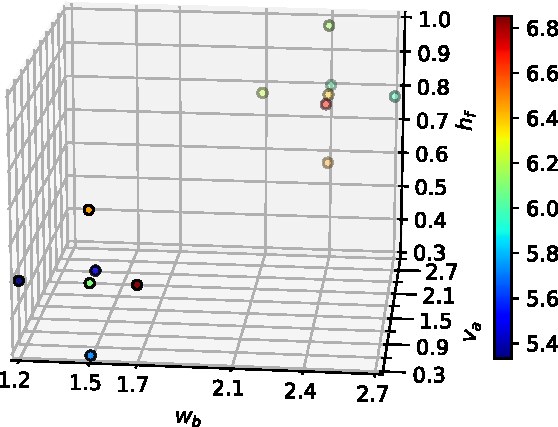
\includegraphics[width=\columnwidth]{sources-testing-straight_sample_points.pdf}
		\caption{Comparison of results to analytical model}
	\end{subfigure}
	\caption{Experimental setup of diagonal design.}
\end{figure}
\fi







\begin{figure}
	\centering
	\begin{subfigure}{.49\columnwidth}
		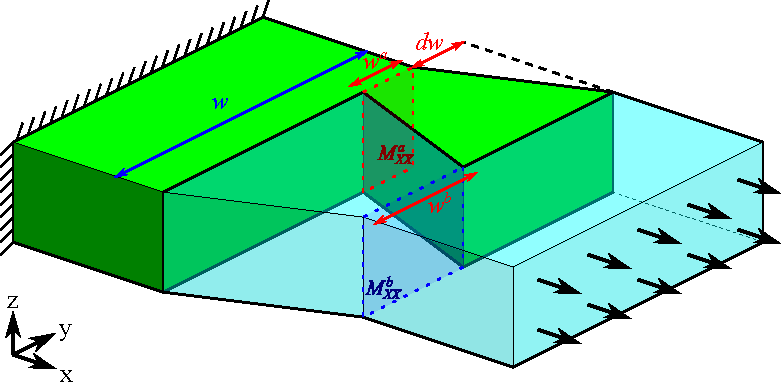
\includegraphics{sources-method-suture_model_v5.pdf}
		\caption{Trapezoidal suture}
		\label{interlocking:fig:suture}
	\end{subfigure}
	\begin{subfigure}{.49\columnwidth}
		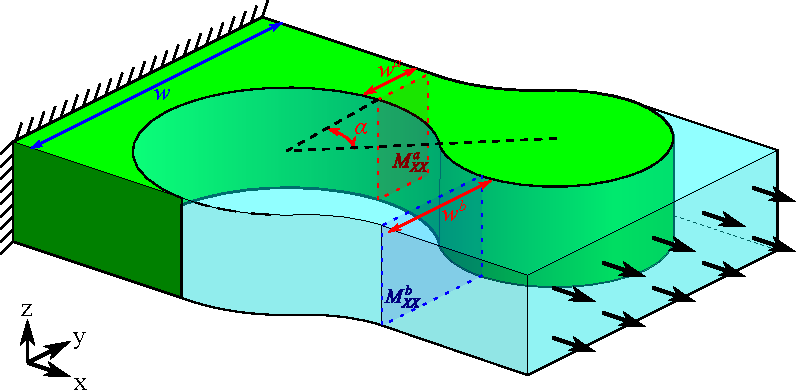
\includegraphics{sources-method-jigsaw_model_v5.pdf}
		\caption{Jigsaw}
		\label{interlocking:fig:jigsaw}
	\end{subfigure}
	\caption{Simple 2D dovetail interlocking microstructures.}
	\label{interlocking:fig:suture_jigsaw}
\end{figure}


\paragraph{Dovetail interlocking}
We compared our interlocking structures against two interlocking designs: trapezoidal sutures and jigsaw interlocking.
See \cref{interlocking:fig:suture_jigsaw}.
We used $\wa=2\wmin{a}$, $dw=\SI{0.3}{\milli\meter}$ and $L=2.4$ for the trapezoidal suture,
and $\wa=2\wmin{a}$ and $\alpha = \SI{35}{\degree}$ for the jigsaw interlocking design.
We printed samples with both $\wb=3\wa$ and $\wb=\nicefrac{\sigmafail{a}}{\sigmafail{b}}\wa = 4.48 \wa$.
%The latter value is optimized for tensile failure along $\myz{b}$. >> not true!!!
We used 6 and 4 repetition respectively and a height of \SI{5}{\milli\meter}.

Note that the jigsaw interlocking structure is quite similar to the trapezoidal suture, with the addition of semicircles to the ends of the trapezoids.
The total length $L$ of the jigsaw structure is \SI{2.96}{\milli\meter} and \SI{4.05}{\milli\meter} for the two $\wb$ values respectively,
so the $\lmax$ constraint is violated by that structure.

The boundaries of these two structures end in half a TPLA lobe, because that is the stiffer material.
In order to meet the minimum width constraint there, the sides of the specimen are extruded by $\wmin{a}$.
However, because the dovetails wider toward the tip, they require an extra toolpath to be filled densely, which is disconnected from the other toolpaths, therefy violating extrusion continuity constraints.
See \cref{interlocking:fig:gcode_suture,interlocking:fig:gcode_jigsaw}



\begin{figure*}
	\centering
	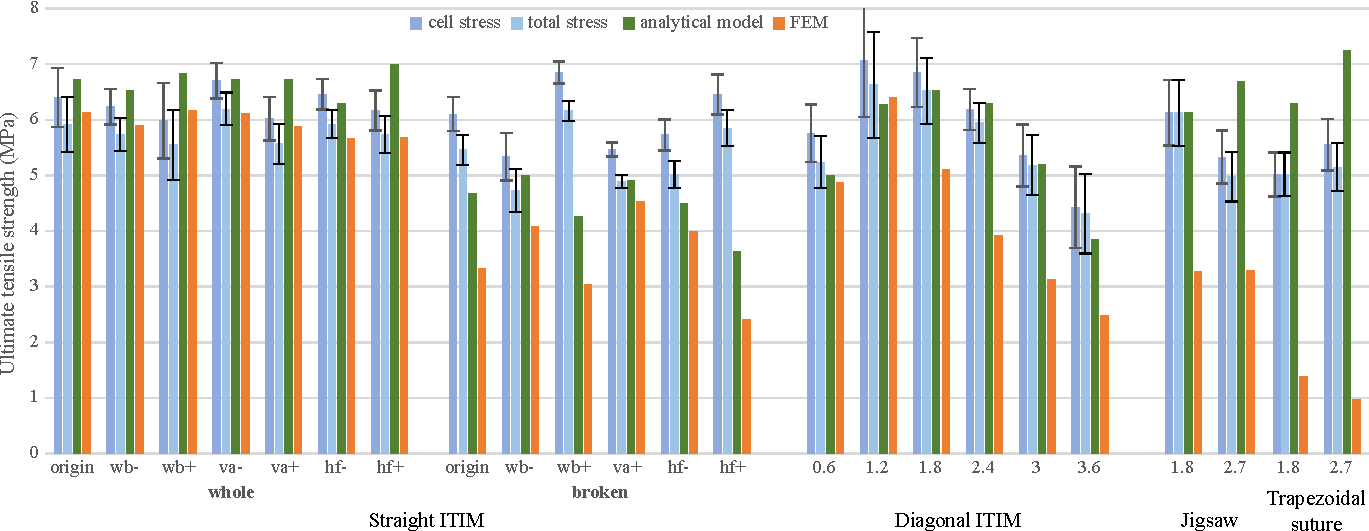
\includegraphics[width=\textwidth]{sources-testing-results.pdf}
	\caption{Test results compared to the predictions according to the analytical model and the RBF network fitted to the simulation results. The straight ITIM variant samples are labelled relative to the whole and broken optimum, while the rest is labelled by their $\wb$ value.}
	\label{interlocking:fig:test_results}
\end{figure*}


\subsubsection{Results}
After tensile testing we can observe various failure modes, such as in \cref{interlocking:fig:failures}.
The tensile tests performed result in force-displacement graphs,
from which the ultimate tensile strength values are derived.
The slope of these graphs after the optimum has been reached furthermore tells us something about the failure mode by which the sample has failed.
See \cref{interlocking:fig:stress_displacement_comparison}.

Because the boundary cells deviate from the regular pattern, computing the ultimate tensile strength can be done in two ways, giving rise to two statistics.
We compute the \emph{cell stress} by dividing the maximum force of the force-displacement graphs by the number of cells and then divide it by the cross sectional area of the cell.
We compute the \emph{total stress} by dividing the force by the total cross-sectional area of the sample, including the extra geometry at the boundaries of the sample.
Ideally we would compensate for manufacturing inaccuracies by using measured dimensions of the specimens,
but measuring the internal geometry of the interlocking structure is practically infeasible, so we use the dimensions of the 3D mesh instead.
The results from the physical experiments, along with the analytical and simulated predictions are gathered in \cref{interlocking:fig:test_results}.


\begin{figure}
	\centering
	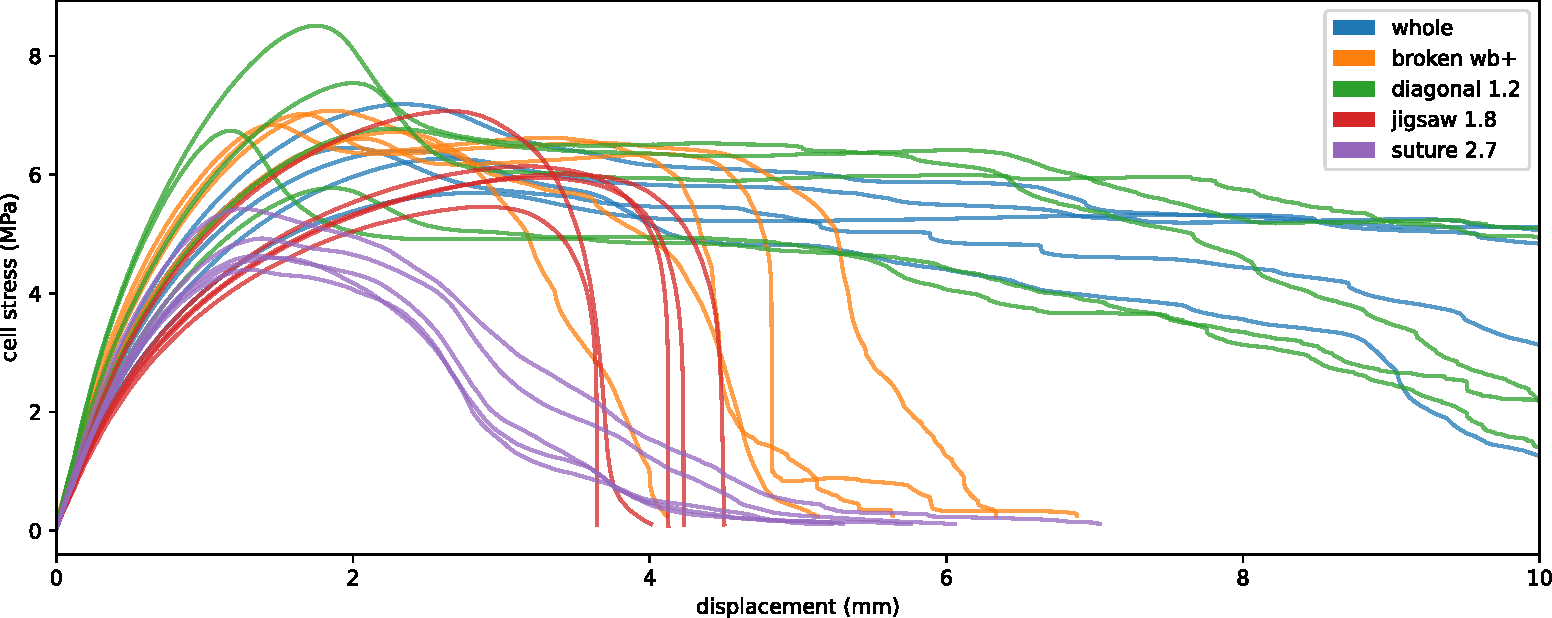
\includegraphics[width=\columnwidth]{sources-testing-stress_displacement_comparison.pdf}
	\caption{Comparison of the best performing design of each type. 
		The diagonal ITIM design with $\wb=\SI{1.2}{\milli\meter}$ showed the highest maximum tensile stress. 
		By inspecting the shape of the graph you can determine the dominant failure mode: TPLA breaking (sharp drop) or PP yielding (plateau).
		Dovetail unlocking has either a sharp drop or a more gradual decline.
	}
	\label{interlocking:fig:stress_displacement_comparison}
\end{figure}



\begin{figure}
	\setlength{\figwidth}{.19\columnwidth}
	\begin{subfigure}[B]{.99\columnwidth}
		\centering
		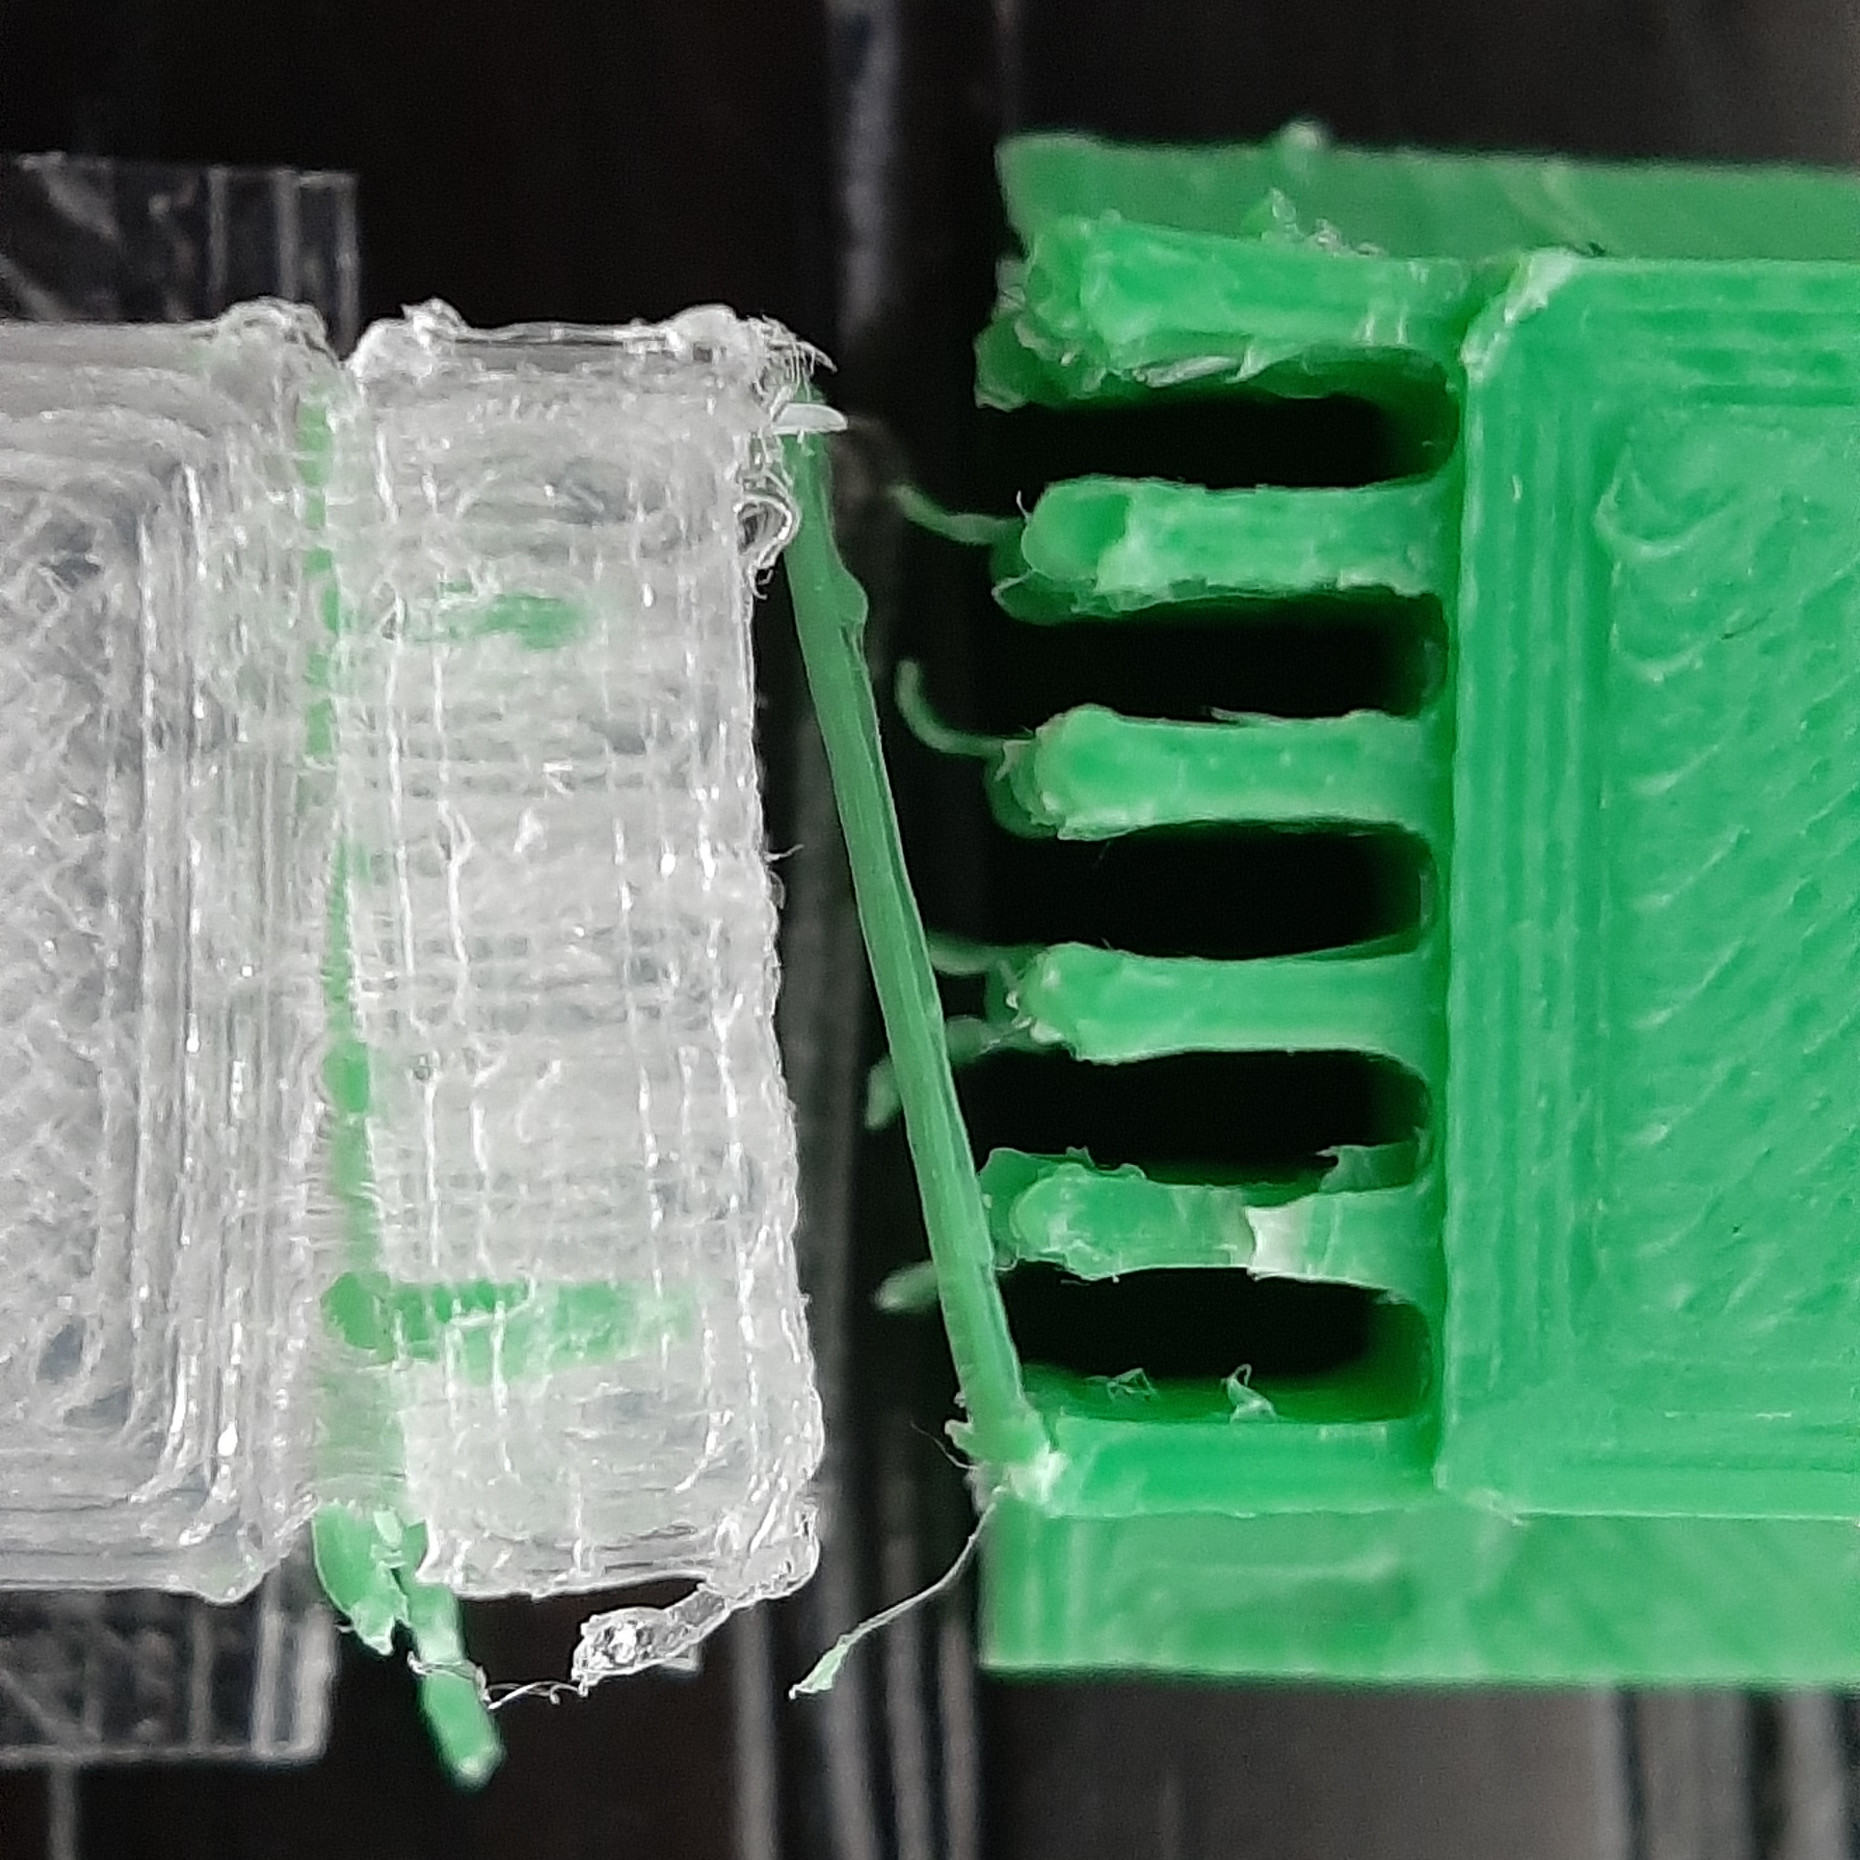
\includegraphics[width=\figwidth]{sources-testing-j1_cropped.jpg}
		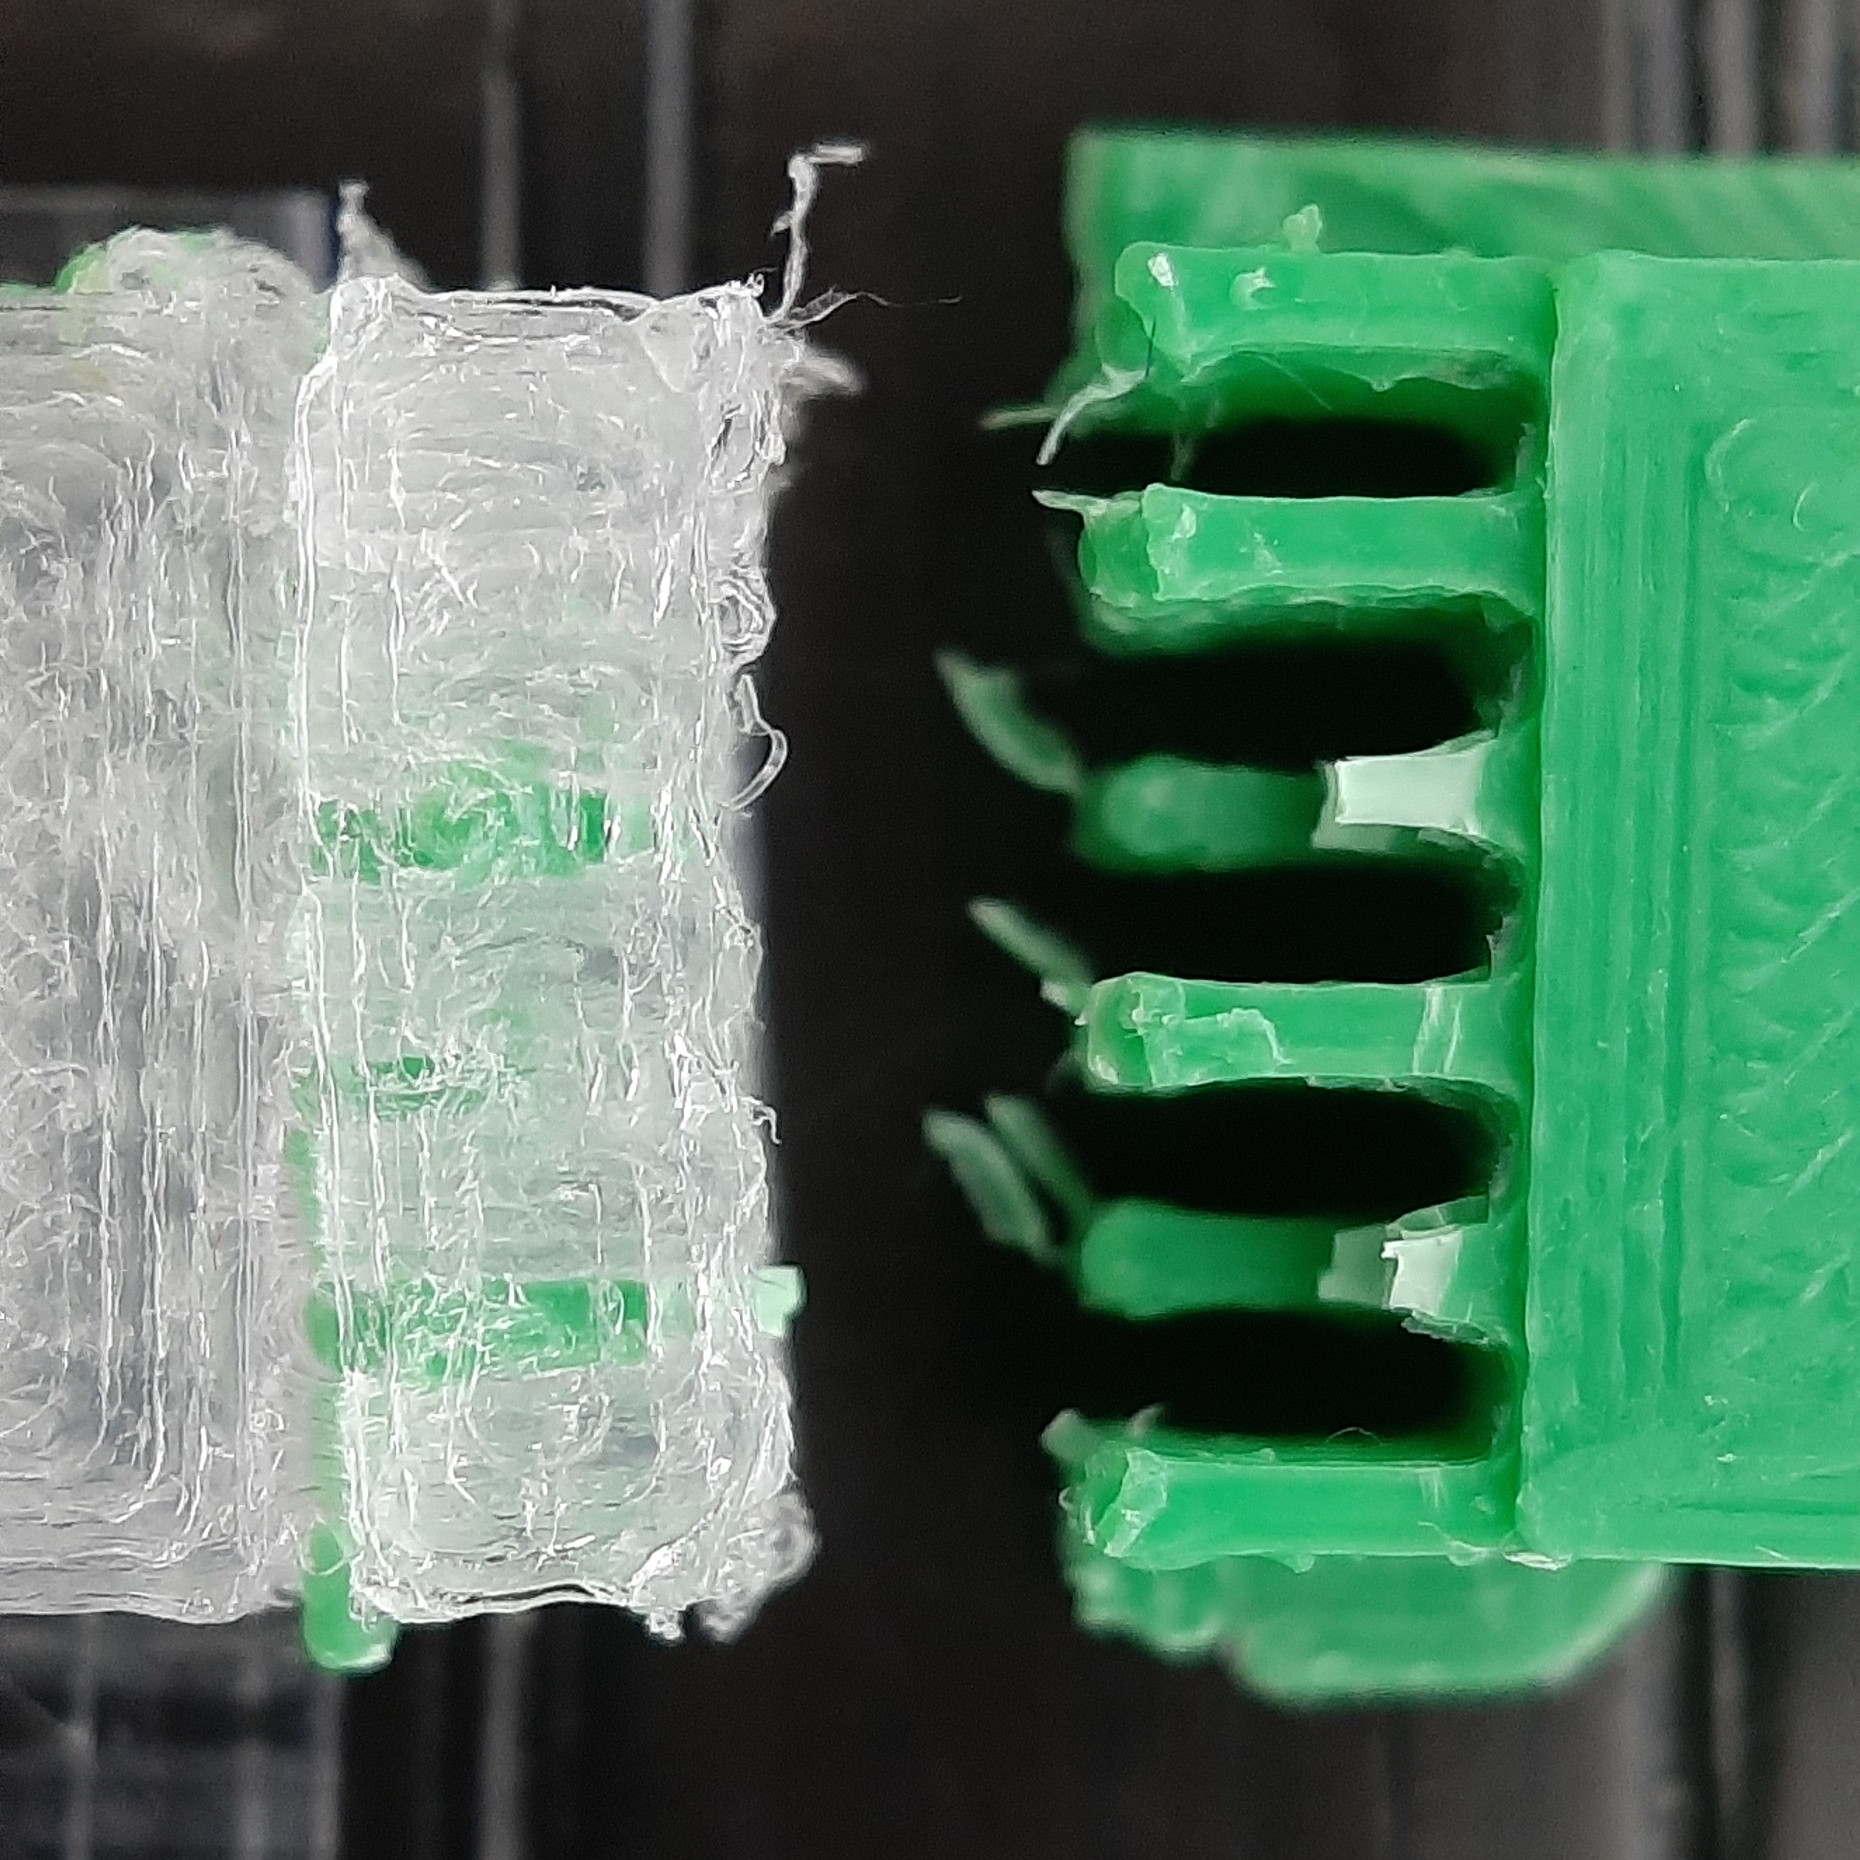
\includegraphics[width=\figwidth]{sources-testing-j2_cropped.jpg}
		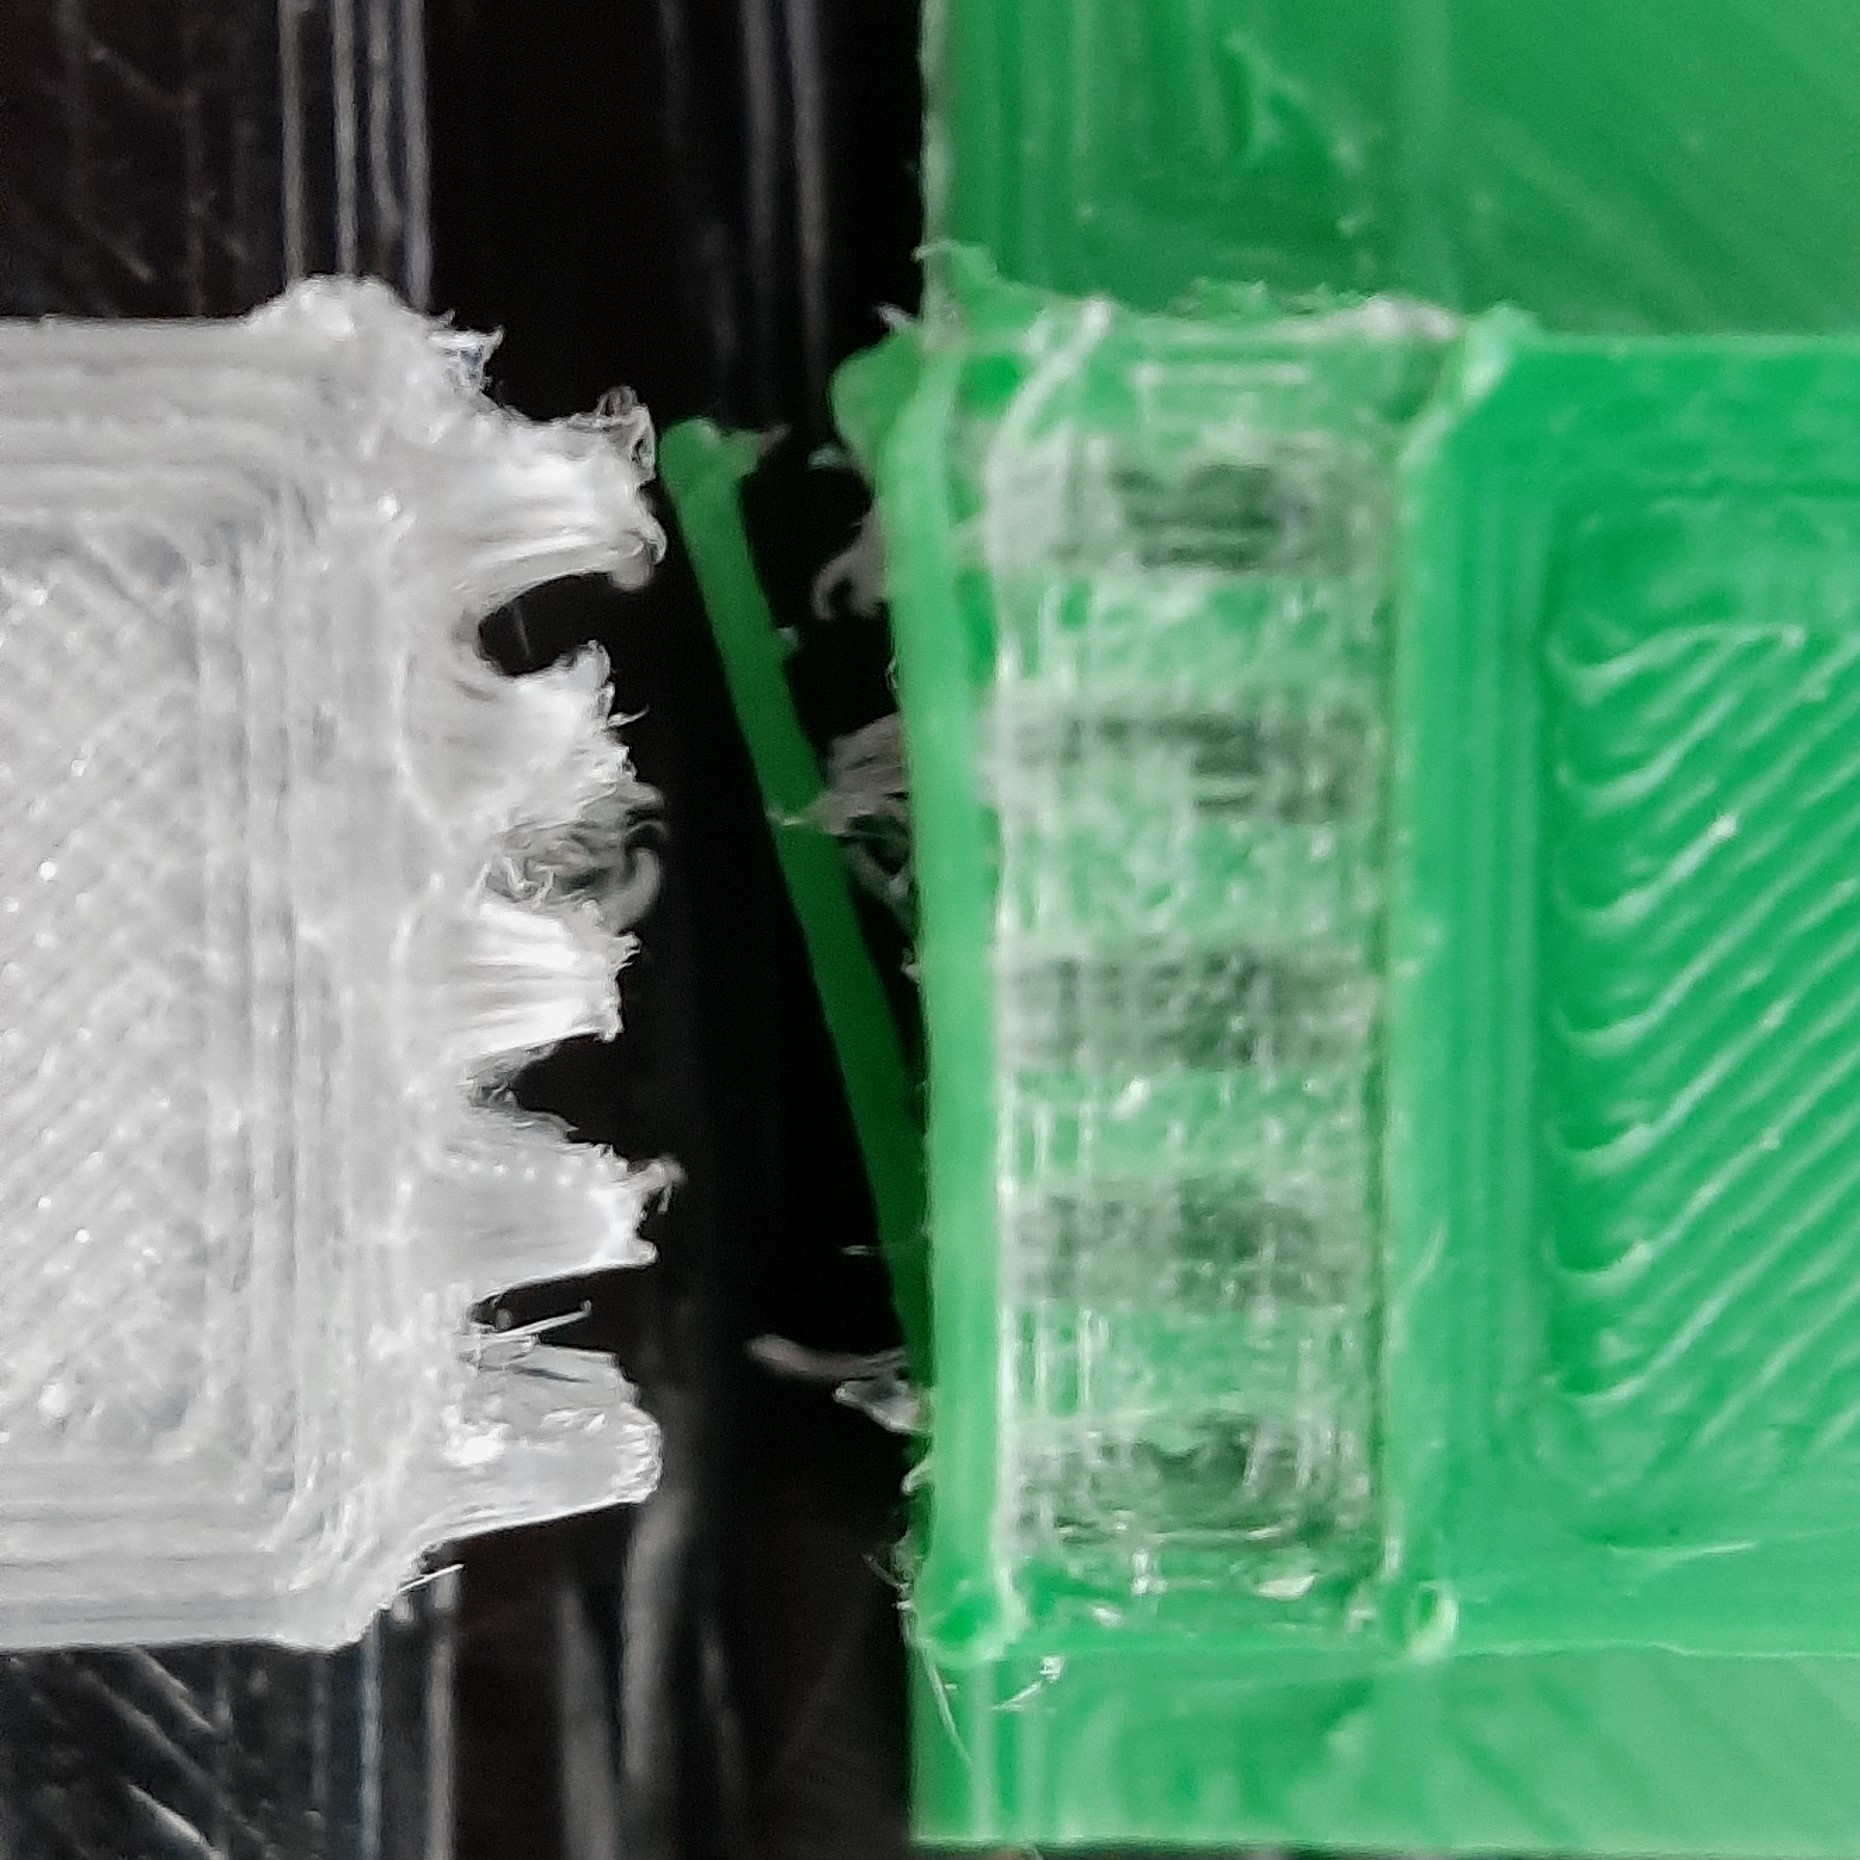
\includegraphics[width=\figwidth]{sources-testing-j3_cropped.jpg}
		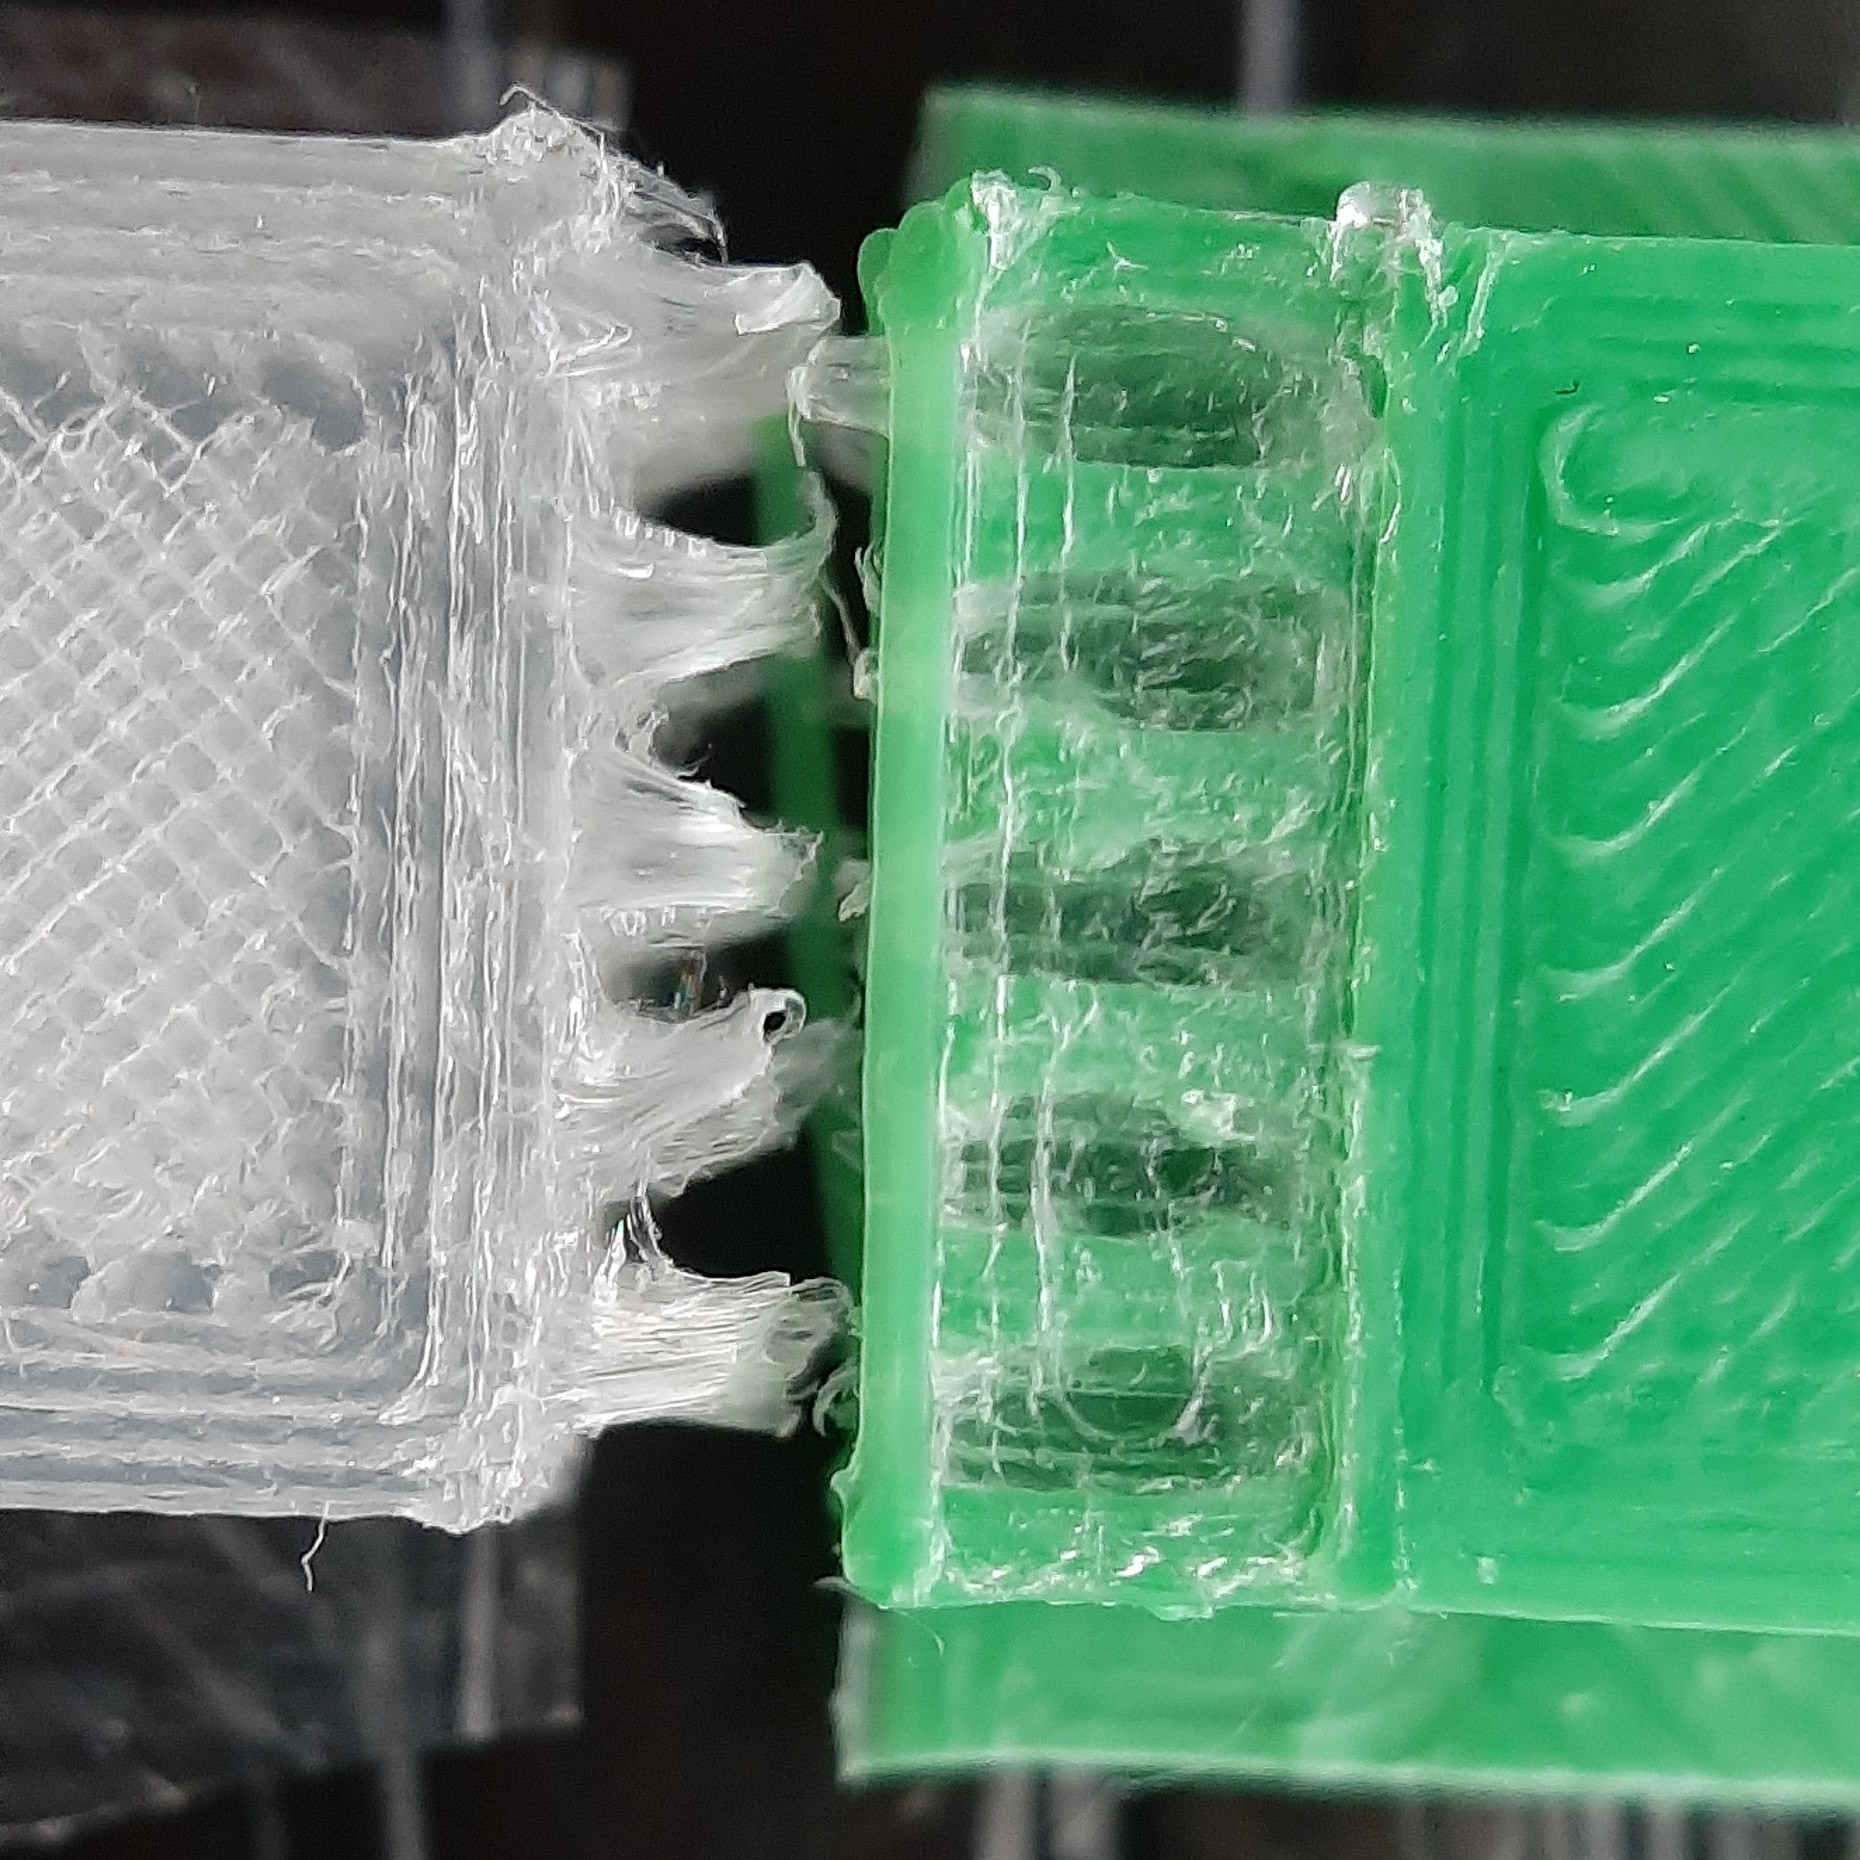
\includegraphics[width=\figwidth]{sources-testing-j4_cropped.jpg}
		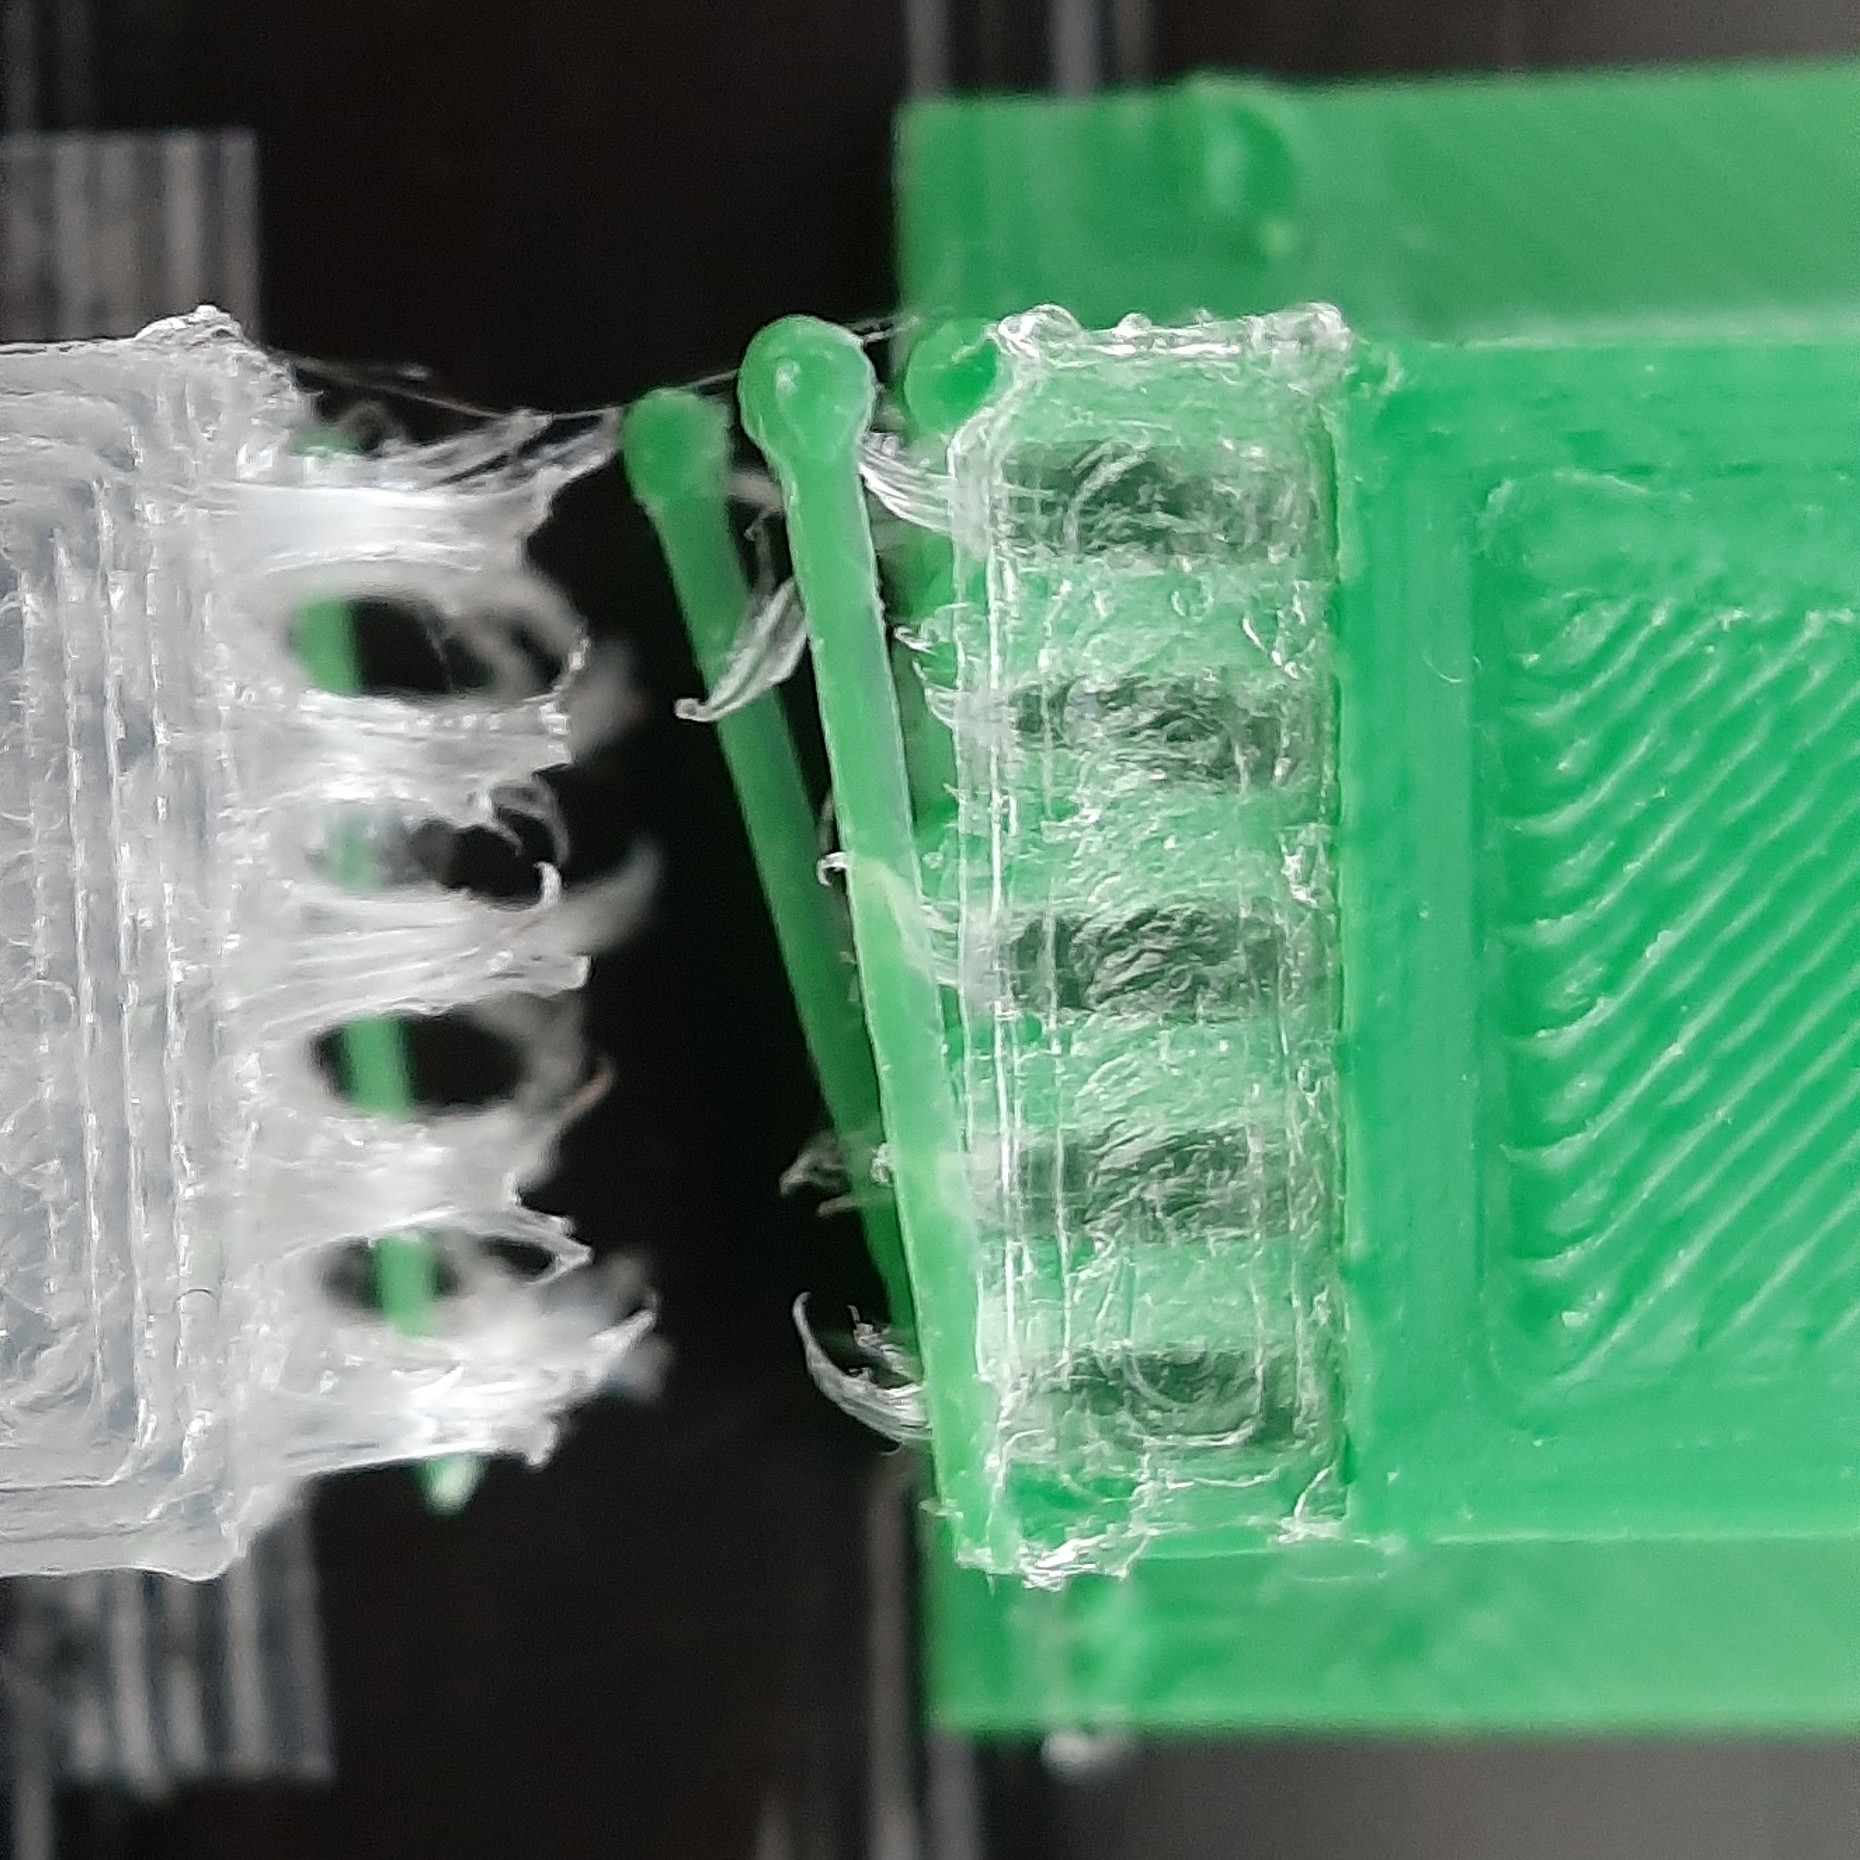
\includegraphics[width=\figwidth]{sources-testing-j5_cropped.jpg}
		\caption{Straight ITIM broken wb+}
		\label{interlocking:fig:failures_straight}
	\end{subfigure}
	\setlength{\figheight}{.25\columnwidth}
	\begin{subfigure}[B]{.28\columnwidth}
		\centering
		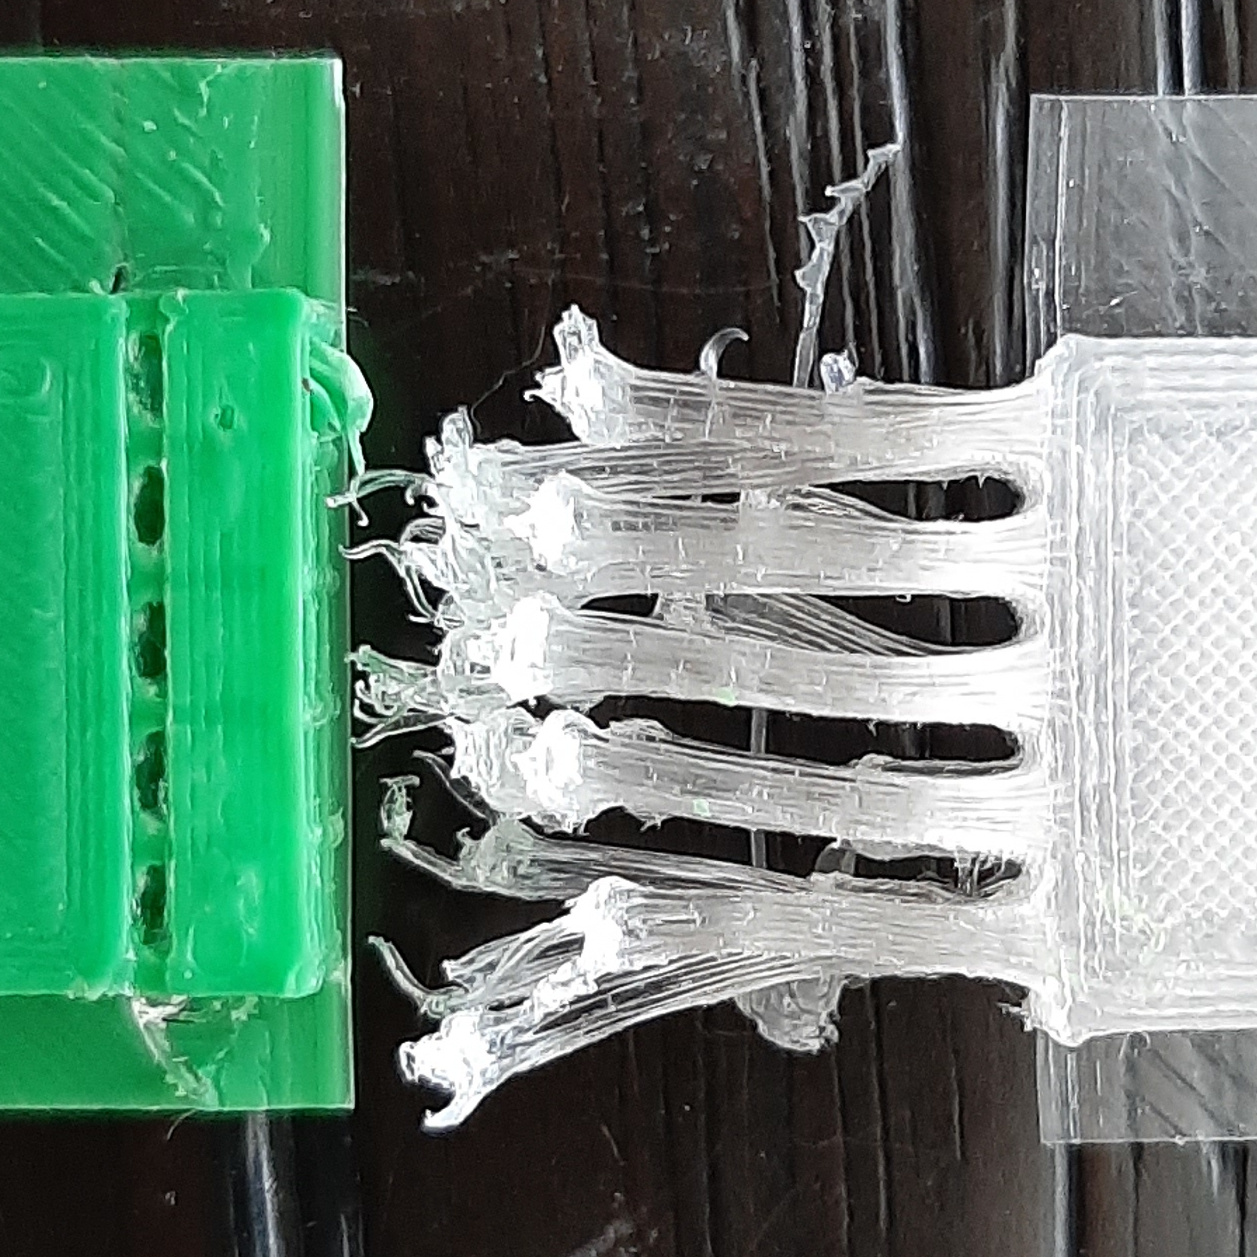
\includegraphics[height=\figheight]{sources-testing-a1_cropped.jpg}
		\caption{Straight ITIM whole}
		\label{interlocking:fig:failures_whole}
	\end{subfigure}
	\begin{subfigure}[B]{.28\columnwidth}
		\centering
		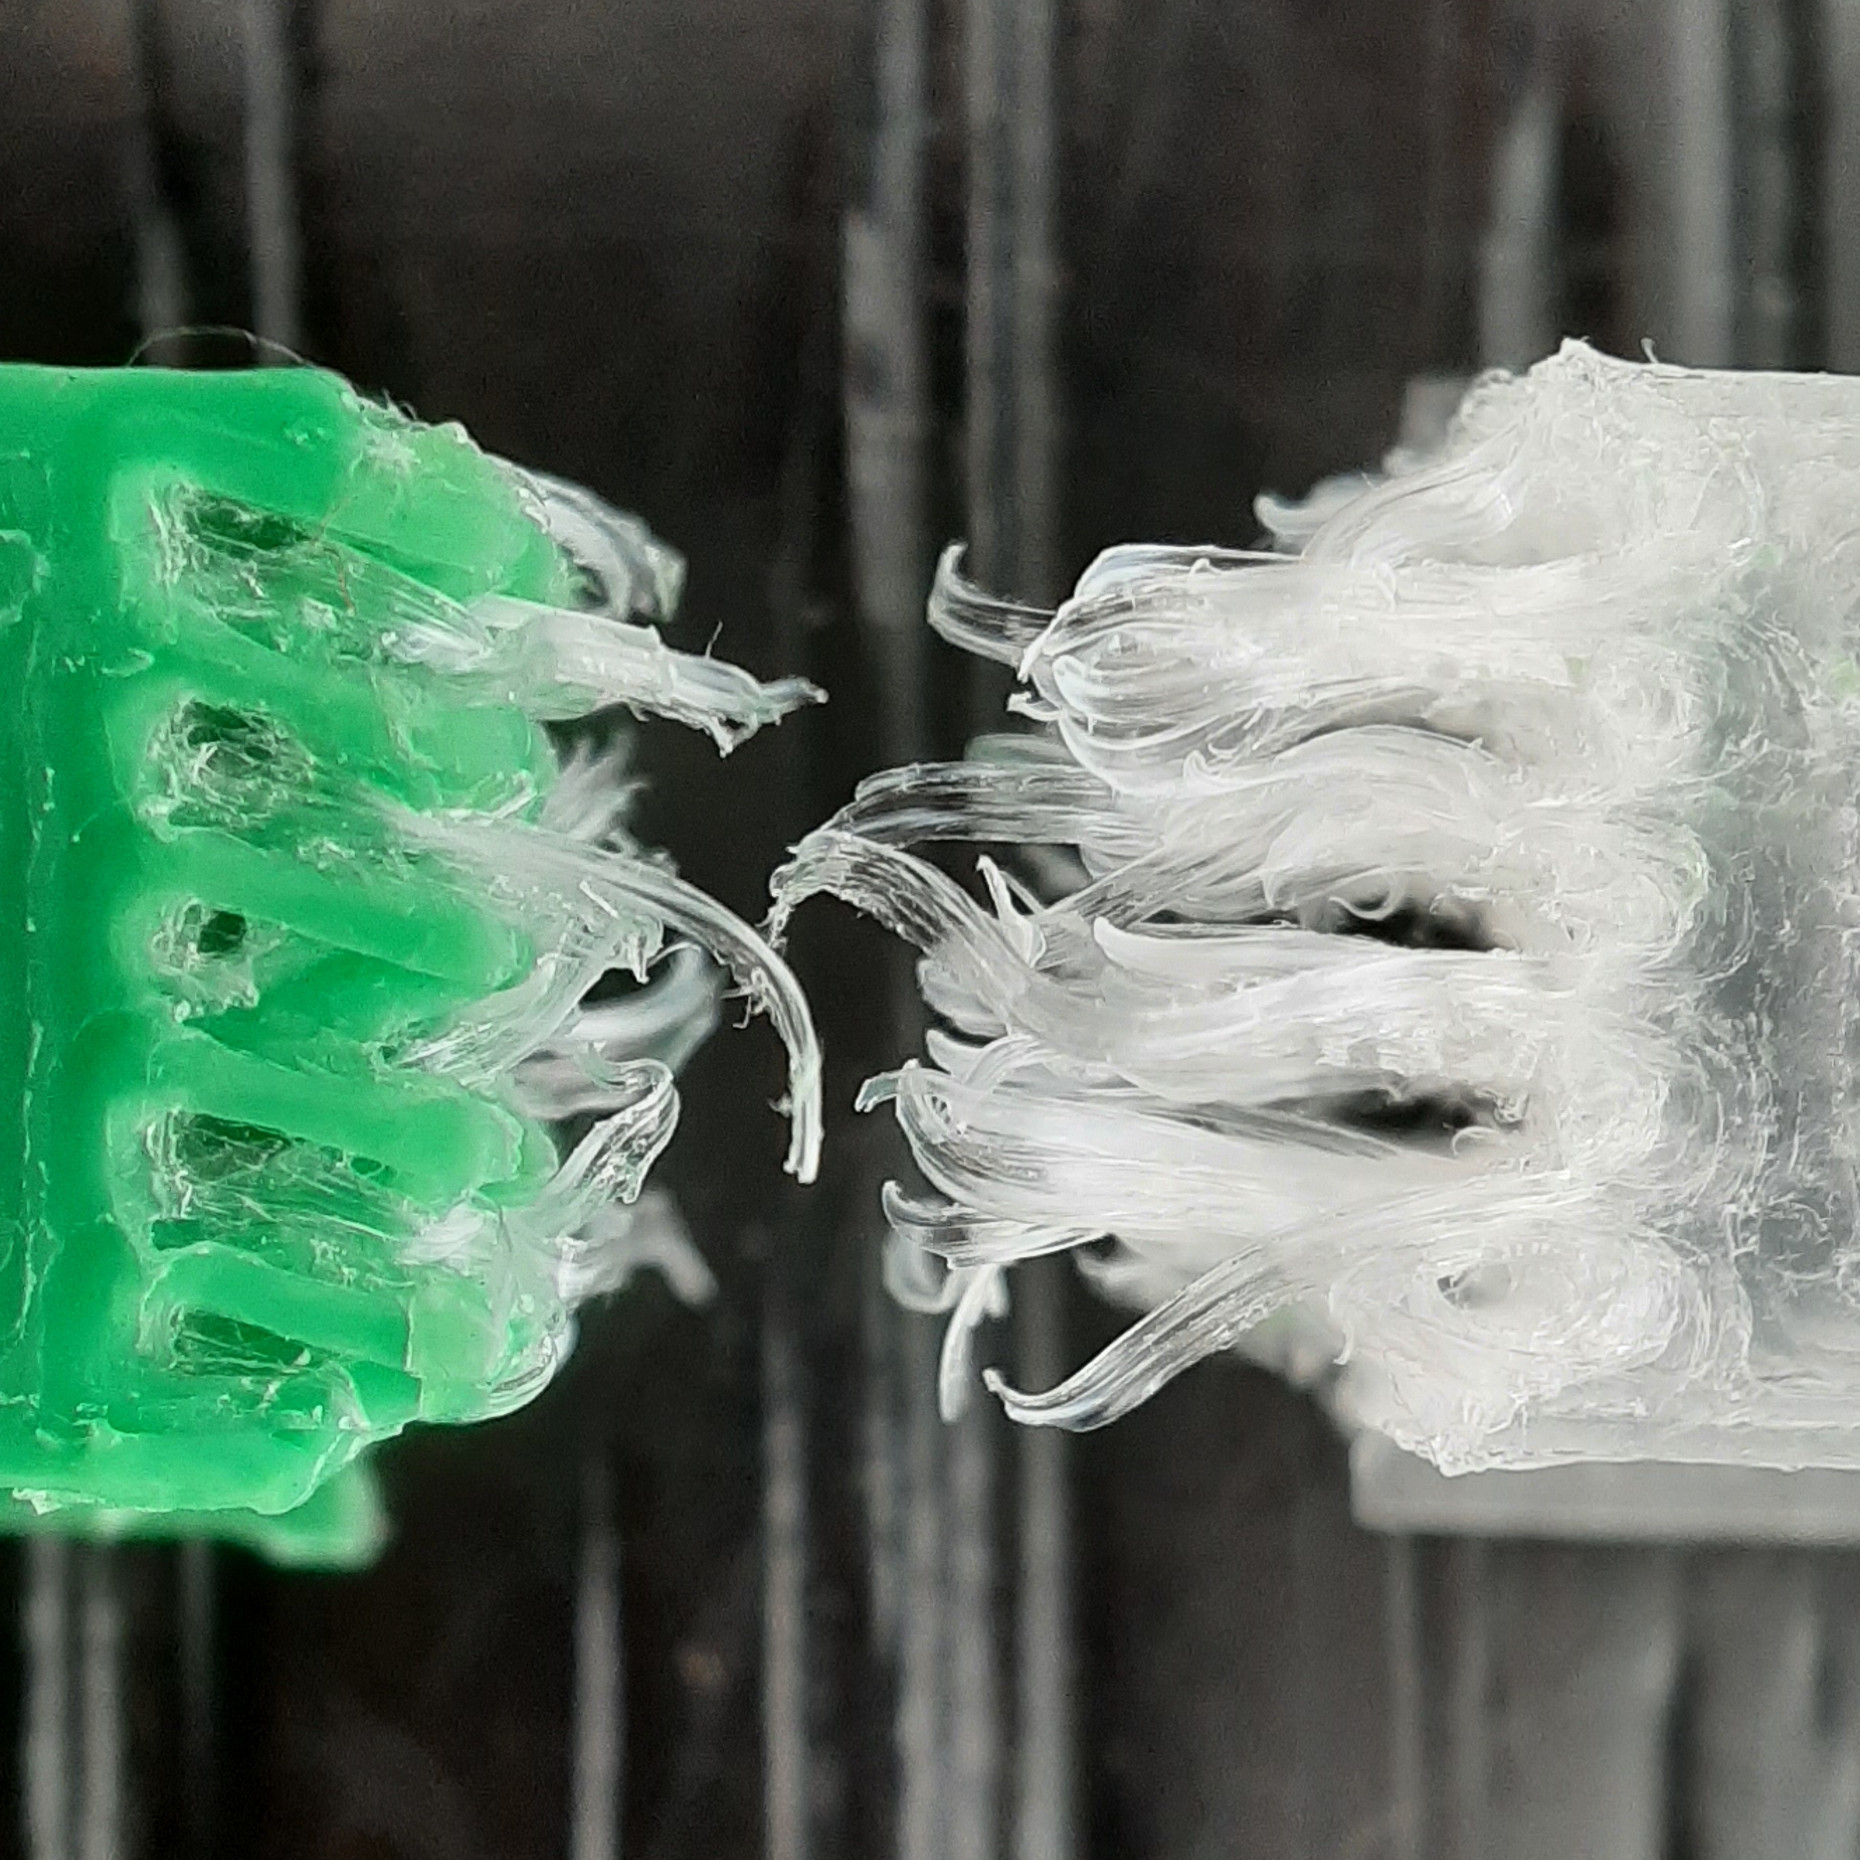
\includegraphics[height=\figheight]{sources-testing-v1_cropped.jpg}
		\caption{Diagonal ITIM $1.2$}
		\label{interlocking:fig:failures_diagonal}
	\end{subfigure}
	\begin{subfigure}[B]{.18\columnwidth}
		\centering
		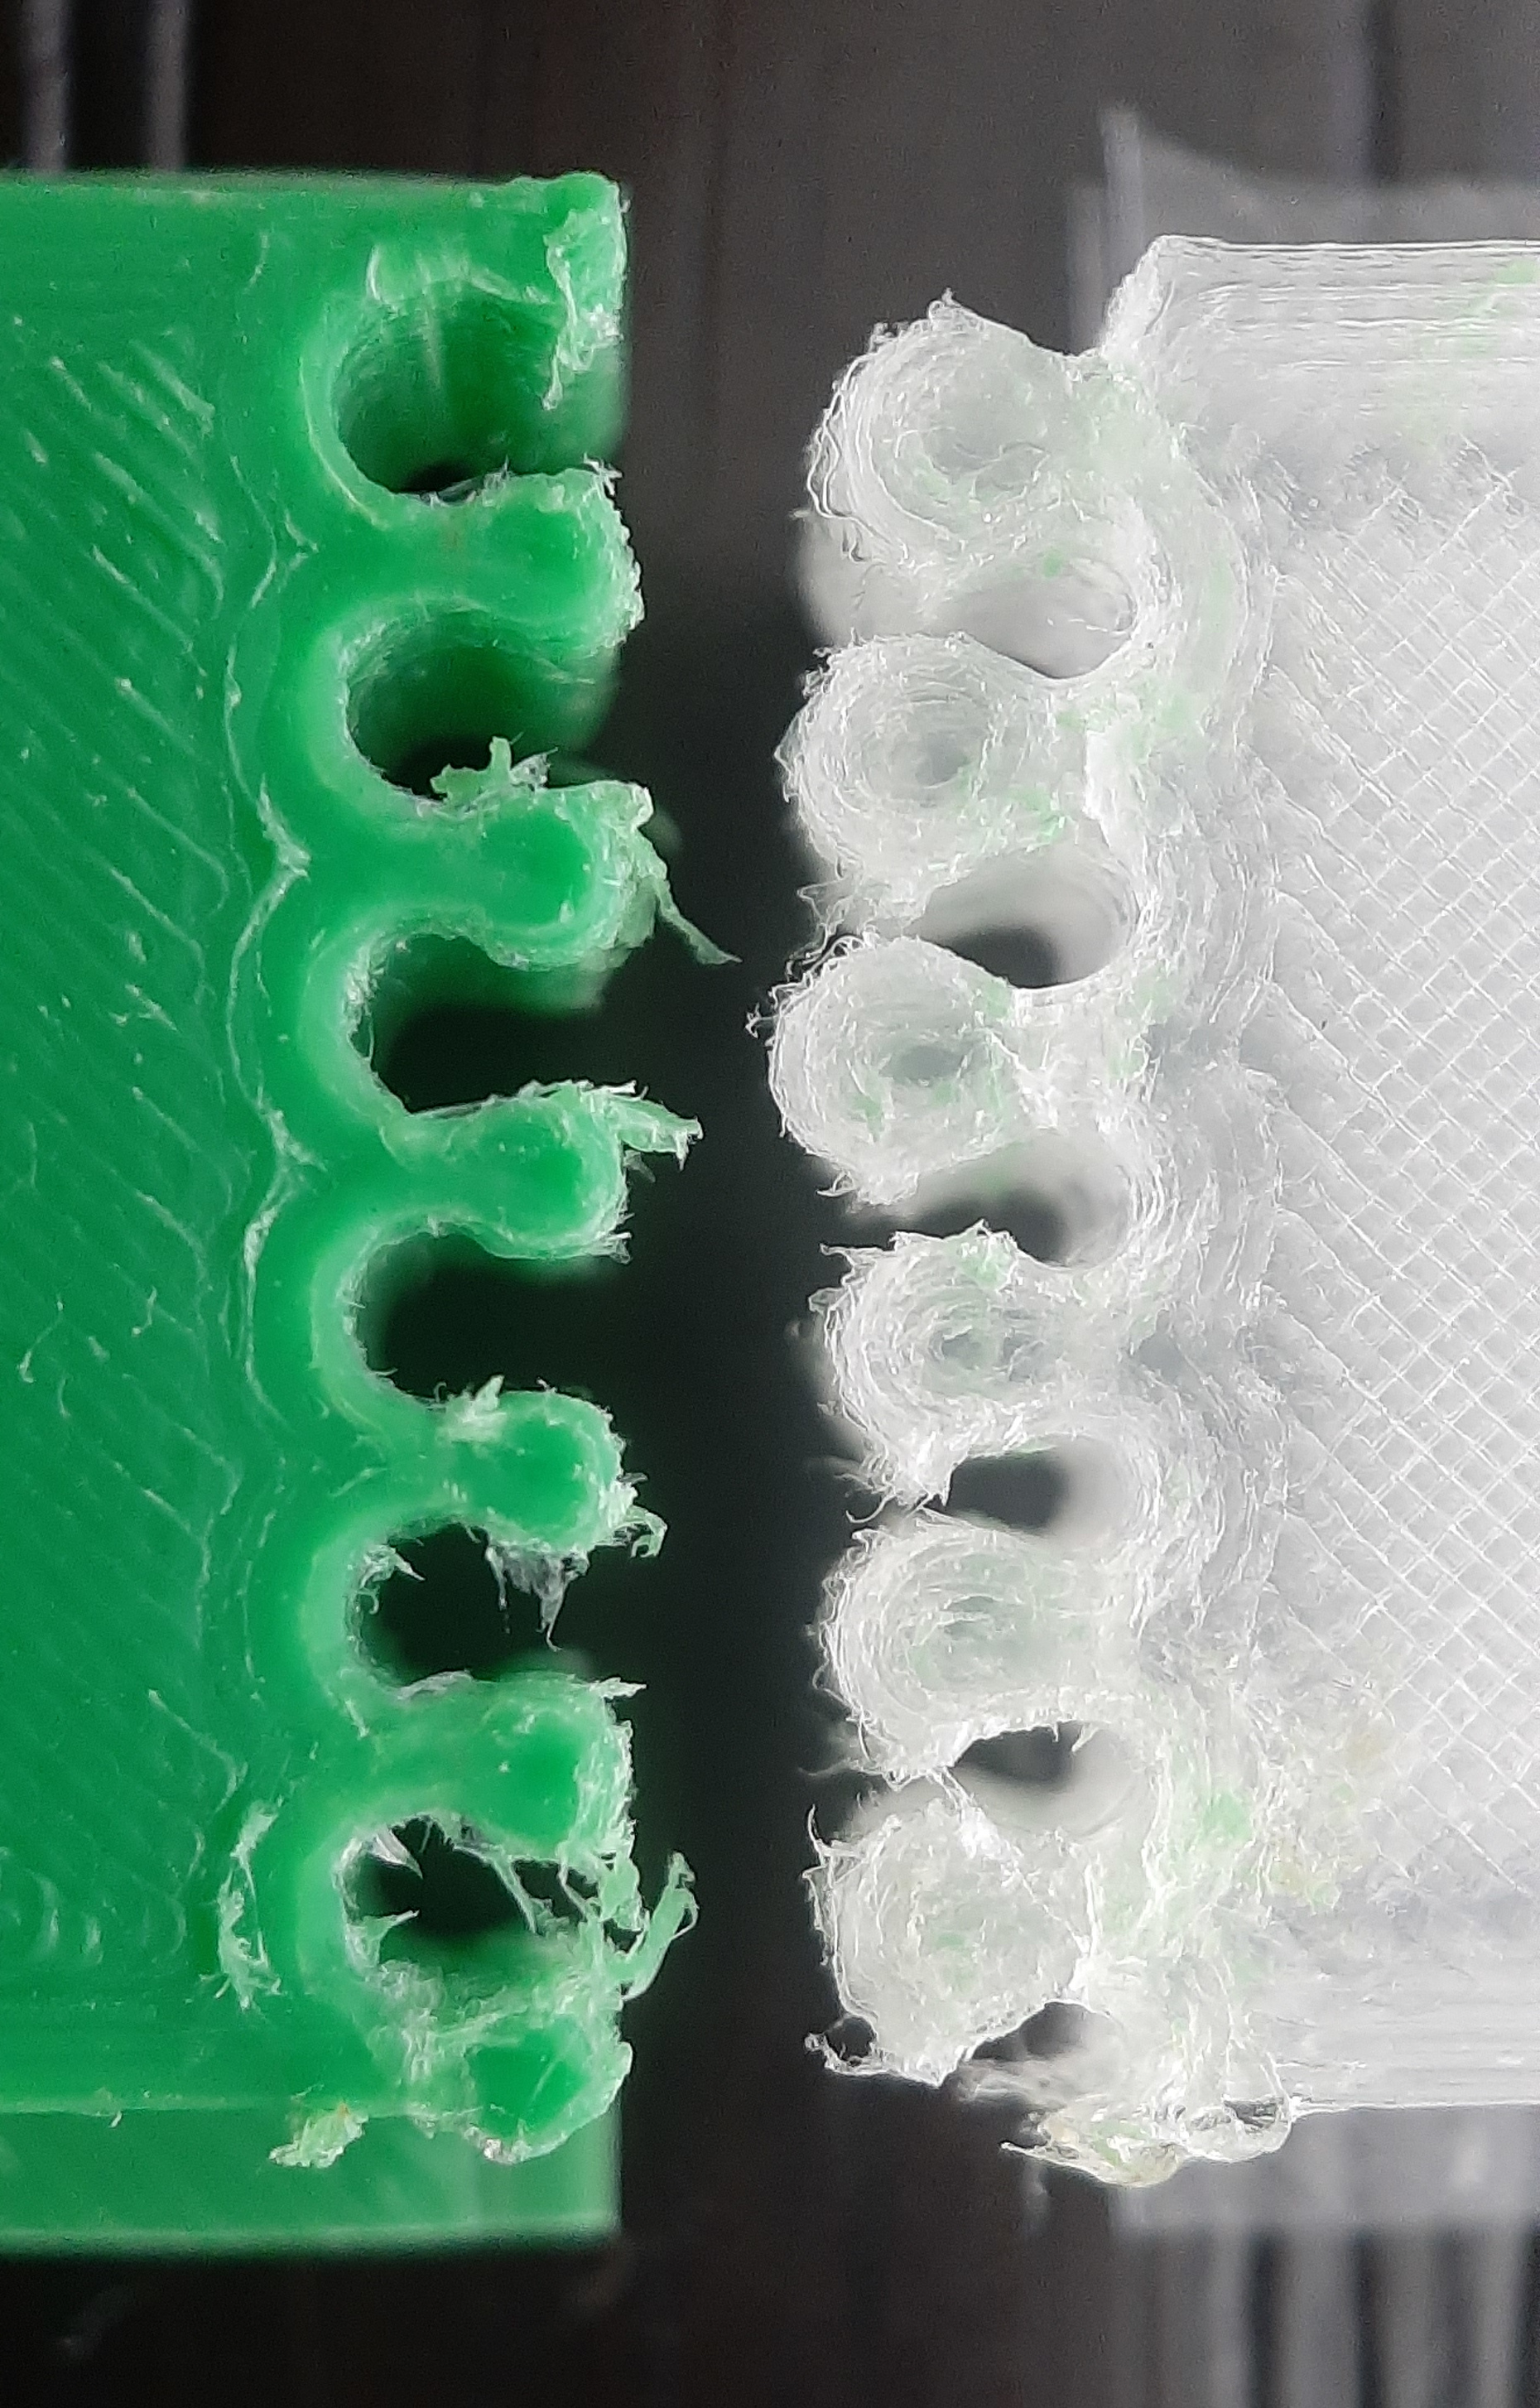
\includegraphics[height=\figheight]{sources-testing-jigsaw_cropped.jpg}
		\caption{Jigsaw $1.8$}
		\label{interlocking:fig:failures_jigsaw}
	\end{subfigure}
	\begin{subfigure}[B]{.22\columnwidth}
		\centering
		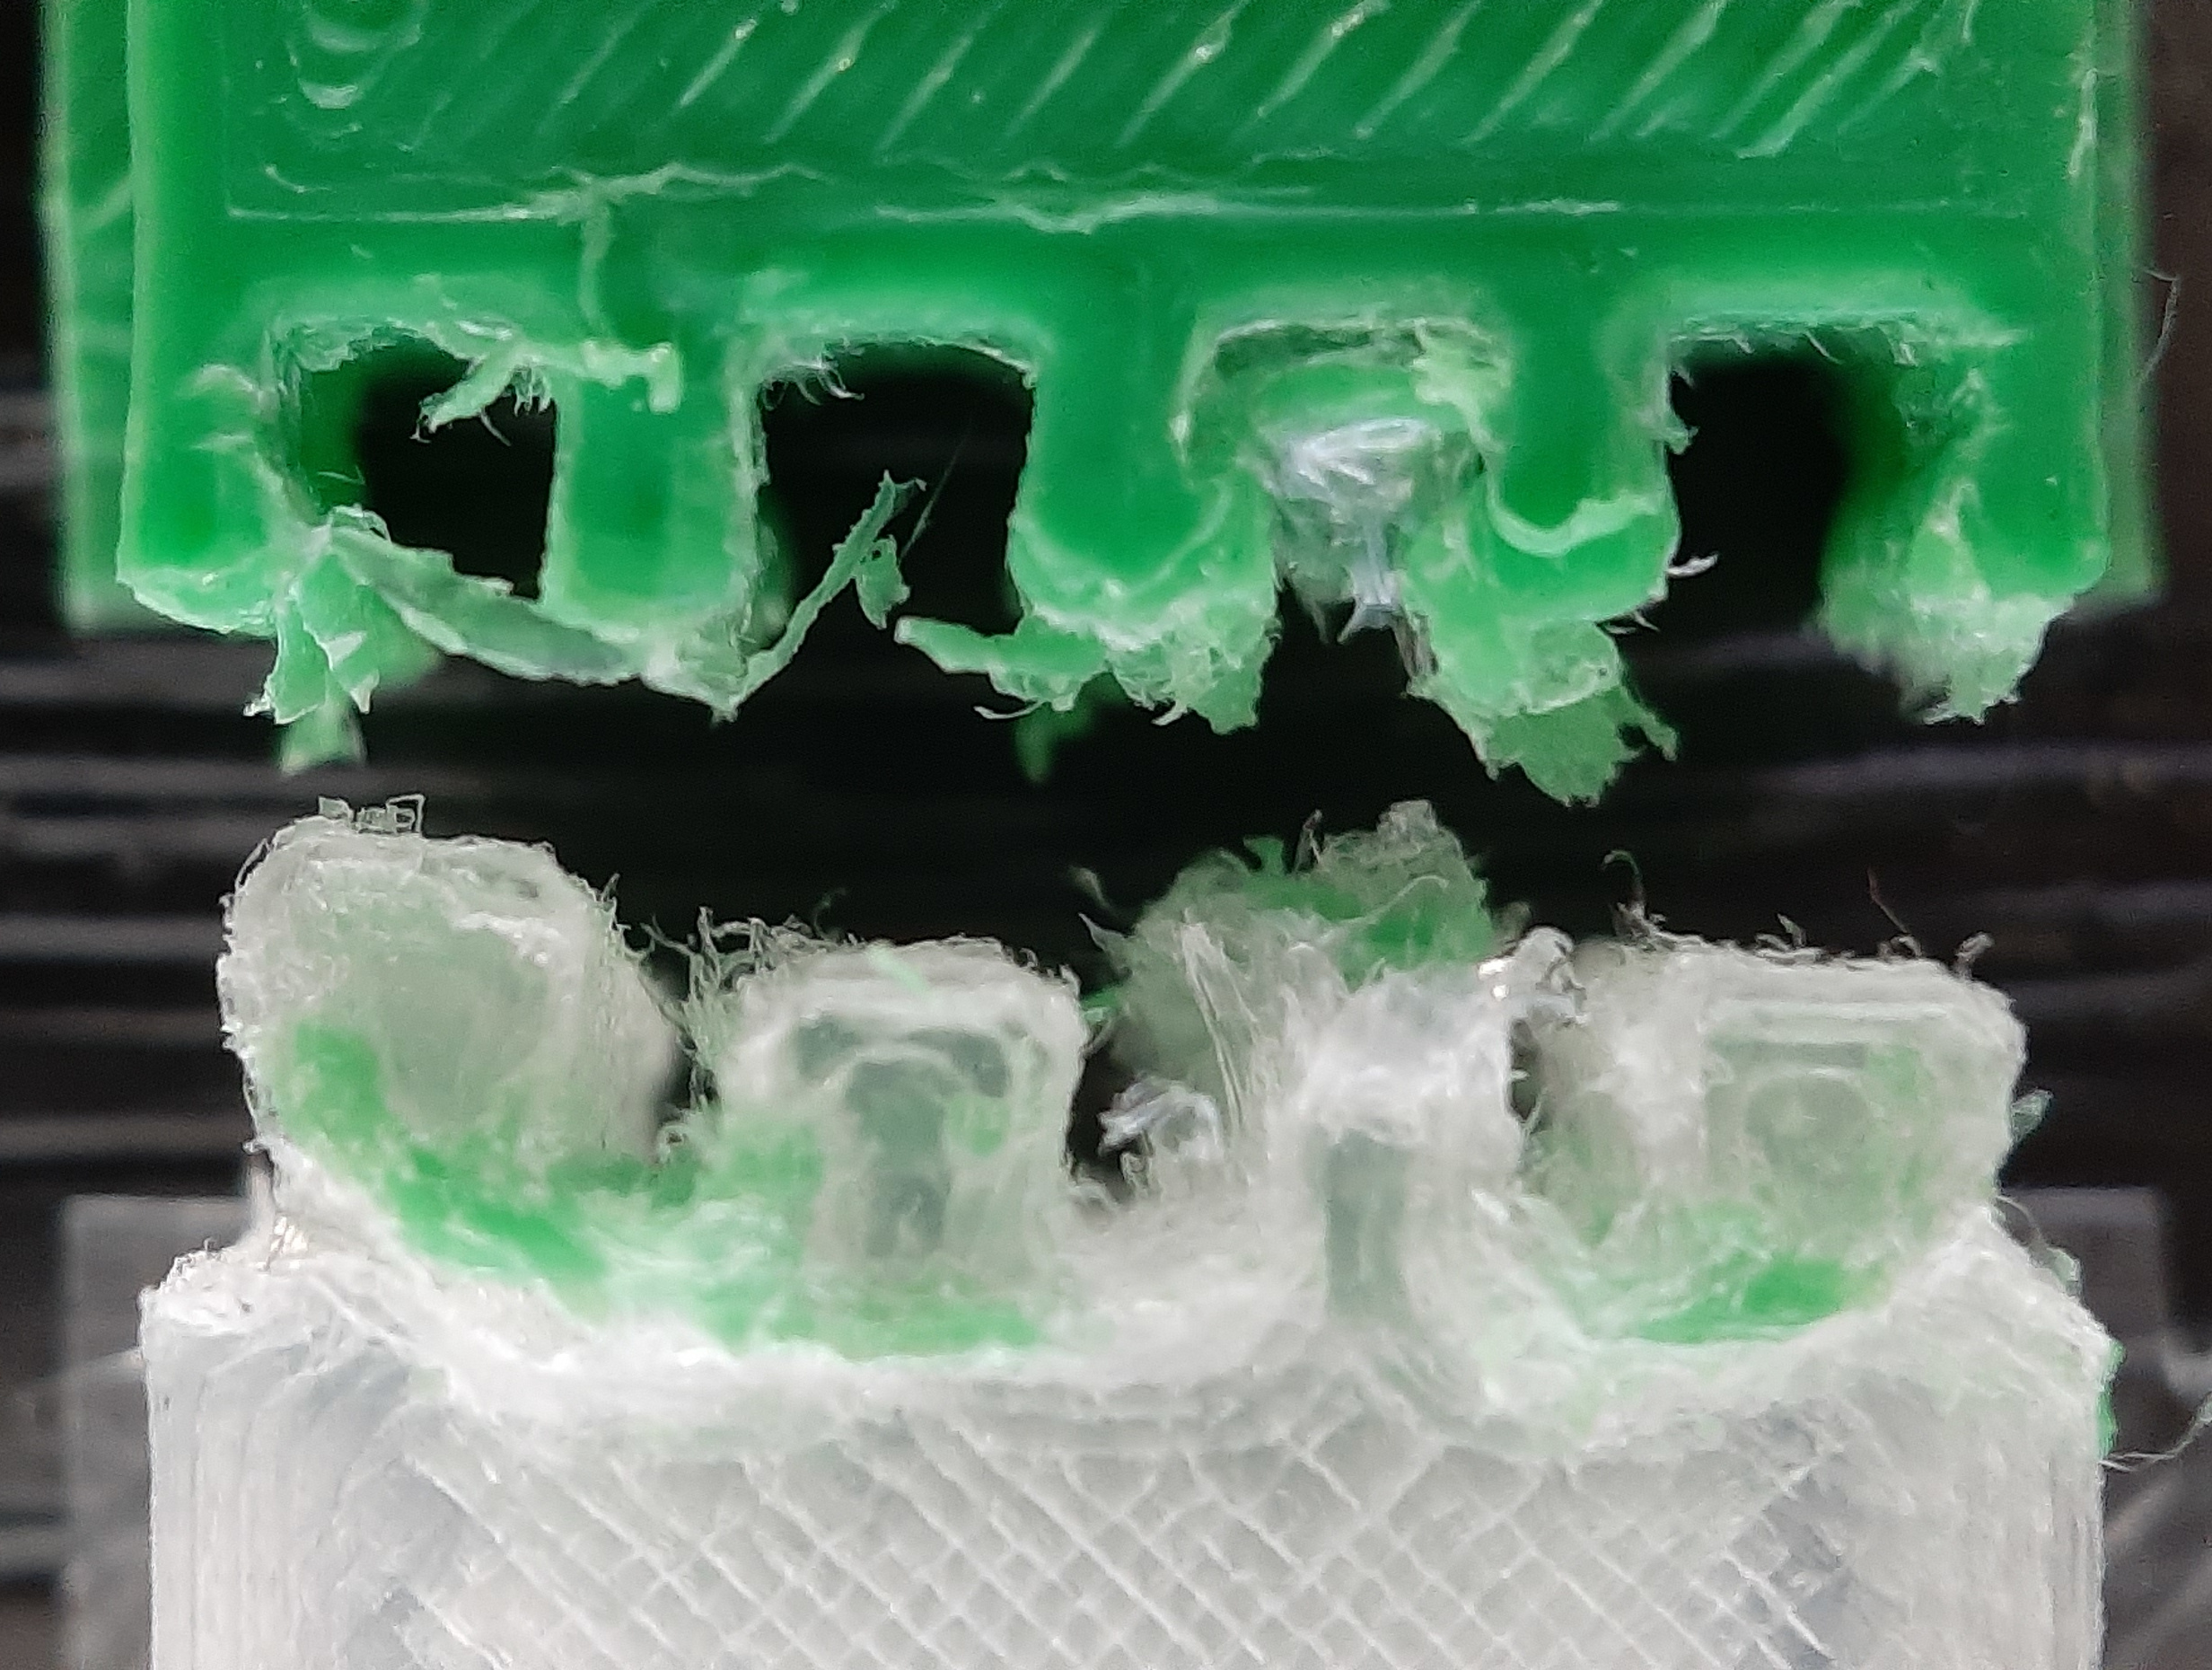
\includegraphics[width=\figheight,rotate=90]{sources-testing-suture_wide_cropped.jpg}
		\caption{Trap. suture $2.7$}
		\label{interlocking:fig:failures_suture}
	\end{subfigure}
	\caption{Samples after tensile tests of the best performing designs.
		The broken wb+ samples from the straight ITIM variant exhibit multiple failure modes, indicating that this sample was close to the intersection of several constraint surfaces.}
	\label{interlocking:fig:failures}
\end{figure}



% table of best sample dimensions?





% !TeX spellcheck = en_GB 
\section{Discussion}
\subsection{Model and simulation validity}
%ana optimum wrt FEM optimum wrt print results

When comparing the tensile test results to the analytical models and the simulation results (\cref{fig:test_results}),
we observe that the whole straight model is predicted rather well by the models.
The analytical model tends to overestimate the strength because of homogeneous stress assumptions,
while the simulations tend to underestimate the strength.
Although the standard deviation is too high to capture the differences in response with significance,
the analytical model follows the trends of the FEM simulations rather well and simulation results generally fall within one standard error of the physical results.
% - perhaps because the tensile properties of the base 3D printing materials were acquired using a different type of toolpathing.

The response around the anticipated optimum of the broken model is predicted by our models considerably worse.
The fact that the simulations performed worse around that area was expected, since after cells in the mesh are broken some self-intersection may occur in the simulation.
When viewing the best performing straight sample (broken wb+, \cref{fig:failures_straight}) we observe that due to manufacturing inaccuracy several failure modes occur throughout the sample,
but shearing off of part of the cross beams is not one of them.
One possible explanation is that for geometry so small as the order of the nozzle size the material properties are closer to the bulk material than to the empirical material properties of printed samples;
the strength determined by the empirical tensile tests relies on the geometry of the toolpaths with which those were printed, while the toolpaths in our interlocking designs might be locally stronger.
Specifically the ITIM toolpaths consist of a small number of long semi-continuous extrusion paths, while %the dovetail designs have discontinuous toolpaths in the wider part of the dovetails.
%In contrast, 
the tensile test specimens with which the material properties were determined were printed using a large bulk of diagonal toolpaths
and because they are printed in a large scale compared to the nozzle size their properties are influenced more by the air gaps in between the extrusions.

Although the anticipated optimum from the simulations of the diagonal design are at the same $\wb$ as the tensile tests,
the simulations seem to underestimate the strength of the design.
This might be related to the limitations in the boundary conditions which were applied, but also to an underestimation of the empirically determined material properties of 3D printed parts.
The analytical model seems to slightly underestimate the PP material as well,
which can be related to the fact that the predicted tensile failure surface $\mt{b}$ overlaps $\mxy{b}$ and thereby doesn't fully disconnect the top of the PP finger from its base.
See \cref{fig:diagonal_model}.

The analytical modelling of the dovetail geometries considers only homogeneous tensile stress,
but disregards the fact that the interlock is broken by deformation alone.
The fact that the dovetail designs don't rely on topological interlocking means that they are more difficult to model.



\subsection{Comparison of interlocking structures}
All interlocking designs considered can reach roughly 6 to \SI{7}{\mega\pascal}, 
which means that $\pm \SI{2}{\mega\pascal}$ of the theoretical upper bound of \SI{8.6}{\mega\pascal} from \cref{eq:general_uper_bound} is used to secure the interlock.
The diagonal design with a cell stress of $7.07 \pm 1.0 \si{\mega\pascal}$ seems to outperform the others, but not significantly.
The dovetail designs performed considerably worse then the other designs - even when the $\lmax$ constraint was violated.
See \cref{fig:stress_displacement_comparison}.

Some designs of the straight ITIM variant near where the broken model is optimal perform significantly better than the other tested straight designs;
given the high dimensionality of the design space it might be the case that there is a straight design in between the whole and broken optima which outperforms the diagonal model nonetheless.

For designs where a lower $\lmax$ is allowed the diagonal orientation performs worse.
For $\lmax=\SI{1.8}{\milli\meter}$ the diagonal is simulated to outperform the straight model by \SI{5.53}{\mega\pascal} to \SI{4.69}{\mega\pascal}.
See \cref{tab:sim_straight_optima}.
The performance of the diagonal model greatly reduces for lower $\lmax$, because the angle of the beams is reduced, which causes them to be more susceptible to shear stresses.





\subsection{Limitations}
The biggest obstacle to drawing definitive conclusions about the relative strengths of the interlocking structures is the size of the standard deviation.
The variation in results has a multitude of causes, related to print head position inaccuracy, filament diameter fluctuations, temperature oscillations and even the location on the print bed.
\footnote{With different locations on the build plate the Bowden tube is bent differently, altering the pressure and thus the amount of extrusion.}
In order to mitigate these factors we have spread out the various geometries over 5 different Ultimaker S5 printers and different locations on the bed.
Although this increases the variability in the results it does increase the reliability.

Because we needed to test a large quantity of samples, we had to limit the size of the samples in terms of interface dimensions.
For the $5\times5$ cells of the straight geometries 12 out of 25 cells were boundary cells, so it is challenging to extrapolate these results to larger interfaces.
Moreover, the different geometries were tested with different amounts of cells, because the cell geometries were very different.
The dovetail designs were modelled without taking friction into account and the size of the interlock ($dw, \alpha$) wasn't optimized for.
This makes it hard to draw definitive conclusions comparing the different interlocking geometries.

Finally, the validity of our models turned out to be limited,
partly because of homogeneity assumptions and partly because we used empirical material properties of 3D prints, rather than simulating how those properties come about.
In order to get more accurate models we could emulate the contact area and polymer entanglement between neighbouring traces,
fit that to the empirically obtained tensile properties and use the resulting fitted model to simulate the structures on a toolpath level.


\subsection{Applications}

What applications are we going to focus on?
Maybe do an application where we do in-situ optimization?

Something with living hinges.

\paragraph{Flexible \& Rigid}
Soft robotics: prosthetic hand, robotic gripper
Living hinges, wheel with tire

Bi-stable mechanisms for buttons.

Pipe with built in rubber ring for sealing

Interesting TPU applications: drive belts

Metamaterials: footwear

\paragraph{Flexible \& Water-absorbent}
Self-regulating systems.

\paragraph{Water-soluble \& Chemically inert}
Automatic substance deployment



% !TeX spellcheck = en_GB 
\section{Conclusion}

interlocking can achieve 85\% of the strength of the PP and TPLA base materials; we reach about 65\%

diagonal design outperforms dovetail interlocking?

genus interlocking shows potential for high compliance materials

genus interlocking can help with complex and slanted surfaces 


\subsection{Applications}
exxplain: PP for living hinges; TPLA for stiffness


photo's of gripper, container, prosthetic hand 



\subsection{Future work}
optimize for different loadings, different materials, different nozzle sizes

optimize for complex surfaces and complex loading situations



investigate 

\interlinepenalty=100000 % prevents pdfendlink ended up accross pages error. see https://tex.stackexchange.com/a/449633/129190
\bibliography{99_mybib}


%\begin{appendices}
%\input{19_edge_discretization}
%\end{appendices}

\end{document}
